%%% Copyright (C) 2018 Vincent Goulet
%%%
%%% Ce fichier fait partie du projet
%%% «Théorie de la crédibilité avec R»
%%% http://github.com/vigou3/theorie-credibilite-avec-r
%%%
%%% Cette création est mise à disposition selon le contrat
%%% Attribution-Partage dans les mêmes conditions 4.0
%%% International de Creative Commons.
%%% http://creativecommons.org/licenses/by-sa/4.0/

\documentclass[letterpaper,11pt,x11names,english,french]{memoir}
  \usepackage{natbib,url}
  \usepackage{babel}
  \usepackage[autolanguage]{numprint}
  \usepackage{amsmath,amsthm}
  \usepackage[noae]{Sweave}
  \usepackage{graphicx}
  \usepackage{rotating}                % env. sideways pour annexe A
  \usepackage{framed}                  % env. snugshade*, oframed
  \usepackage[absolute]{textpos}       % éléments des pages de titre
  \usepackage[shortlabels]{enumitem}   % configuration listes
  \usepackage{relsize}                 % \smaller et al.
  \usepackage{manfnt}                  % \mantriangleright (puce)
  \usepackage{metalogo}                % \XeLaTeX logo
  \usepackage{fontawesome}             % icônes \fa*
  \usepackage{awesomebox}              % boites info, important, etc.
  \usepackage{answers}                 % exercices et solutions
  \usepackage{listings}                % code informatique
  \usepackage{pgf}                     % transparence pour couverture avant

  %%% =============================
  %%%  Informations de publication
  %%% =============================
  \title{Théorie de la crédibilité avec R}
  \author{Vincent Goulet}
  \renewcommand{\year}{2018}
  \renewcommand{\month}{01-1}
  \newcommand{\ghurl}{https://github.com/vigou3/theorie-credibilite-avec-r/}

  %%% ===================
  %%%  Style du document
  %%% ===================

  %% Polices de caractères
  \usepackage{fontspec}
  \usepackage{unicode-math}
  \defaultfontfeatures{Scale=0.92}
  \setmainfont[Ligatures=TeX,Numbers=OldStyle]{Lucida Bright OT}
  \setmathfont{Lucida Bright Math OT}
  \setmonofont{Lucida Grande Mono DK}
  \setsansfont[Scale=1.0,Numbers=OldStyle]{Myriad Pro}
  \newfontfamily\fullcaps[Letters=Uppercase,Numbers=Uppercase]{Myriad Pro}
  \usepackage[babel=true]{microtype}
  \usepackage{icomma}

  %% Couleurs
  \usepackage{xcolor}
  \definecolor{comments}{rgb}{0.7,0,0}      % commentaires
  \definecolor{link}{rgb}{0,0.4,0.6}        % liens internes
  \definecolor{url}{rgb}{0.6,0,0}           % liens externes
  \definecolor{citation}{rgb}{0,0.5,0}      % citations
  \definecolor{codebg}{named}{LightYellow1} % fond code R
  \definecolor{darkblue}{rgb}{0,0,0.7}      % pour théorème 4.1
  \colorlet{darkred}{comments}              % idem
  \colorlet{darkgreen}{citation}            % idem
  \definecolor{rouge}{rgb}{0.85,0,0.07} % rouge bandeau identitaire
  \definecolor{or}{rgb}{1,0.8,0}        % or bandeau identitaire

  %% Hyperliens
  \usepackage{hyperref}
  \hypersetup{%
    pdfauthor = \theauthor,
    pdftitle = \thetitle,
    colorlinks = true,
    linktocpage = true,
    urlcolor = {url},
    linkcolor = {link},
    citecolor = {citation},
    pdfpagemode = {UseOutlines},
    pdfstartview = {Fit}}
  \setlength{\XeTeXLinkMargin}{1pt}

  %% Affichage de la table des matières du PDF
  \usepackage{bookmark}
  \bookmarksetup{%
    open = true,
    depth = 3,
    numbered = true}

  %% Étiquettes de \autoref (redéfinitions compatibles avec babel).
  %% Attention! Les % à la fin des lignes sont importants sinon des
  %% blancs apparaissent dès que la commande \selectlanguage est
  %% utilisée... comme dans la bibliographie, par exemple.
  \addto\extrasfrench{%
    \def\appendixautorefname{annexe}%
    \def\figureautorefname{figure}%
    \def\exempleautorefname{exemple}%
    \def\exerciceautorefname{exercice}%
    \def\subfigureautorefname{figure}%
    \def\subsectionautorefname{section}%
    \def\subtableautorefname{tableau}%
    \def\tableautorefname{tableau}%
    \def\thmautorefname{théorème}%
  }

  %% Table des matières (inspirée de classicthesis.sty)
  \renewcommand{\cftchapterleader}{\hspace{1.5em}}
  \renewcommand{\cftchapterafterpnum}{\cftparfillskip}
  \renewcommand{\cftsectionleader}{\hspace{1.5em}}
  \renewcommand{\cftsectionafterpnum}{\cftparfillskip}

  %% Titres des chapitres
  \chapterstyle{hangnum}
  \renewcommand{\chaptitlefont}{\normalfont\Huge\sffamily\bfseries\raggedright}

  %% Marges, entêtes et pieds de page
  \setlength{\marginparsep}{7mm}
  \setlength{\marginparwidth}{13mm}
  \setlength{\headwidth}{\textwidth}
  \addtolength{\headwidth}{\marginparsep}
  \addtolength{\headwidth}{\marginparwidth}

  %% Titres des sections et sous-sections
  \setsecheadstyle{\normalfont\Large\sffamily\bfseries\raggedright}
  \setsubsecheadstyle{\normalfont\large\sffamily\bfseries\raggedright}
  \maxsecnumdepth{subsection}
  \setsecnumdepth{subsection}

  %% Listes. Paramétrage avec enumitem.
  \setlist[enumerate]{leftmargin=*,align=left}
  \setlist[enumerate,2]{label=\alph*),labelsep=*,leftmargin=1.5em}
  \setlist[enumerate,3]{label=\roman*),labelsep=*,leftmargin=1.5em,align=right}
  \setlist[itemize]{leftmargin=*,align=left}

  %% Options de babel
  \frenchbsetup{CompactItemize=false,%
    ThinSpaceInFrenchNumbers=true,
    ItemLabeli=\mantriangleright,
    ItemLabelii=\textendash,
    og=«, fg=»}
  \addto\captionsfrench{\def\figurename{{\scshape Fig.}}}
  \addto\captionsfrench{\def\tablename{{\scshape Tab.}}}

  %%% =========================
  %%%  Sections de code source
  %%% =========================
  \lstloadlanguages{R}
  \lstset{language=R,
    extendedchars=true,
    basicstyle=\small\ttfamily\NoAutoSpacing,
    commentstyle=\color{comments}\slshape,
    keywordstyle=\mdseries,
    showstringspaces=false}

  %%% =========================
  %%%  Nouveaux environnements
  %%% =========================

  %% Environnements d'exemples et al.
  \theoremstyle{plain}
  \newtheorem{thm}{Théorème}[chapter]
  \newtheorem{corrolaire}{Corollaire}[chapter]

  \theoremstyle{definition}
  \newtheorem*{definition}{Définition}
  \newtheorem{exemple}{Exemple}[chapter]

  \theoremstyle{remark}
  \newtheorem*{rem}{Remarque}
  \newtheorem*{rems}{Remarques}

  %% Redéfinition de l'environnement titled-frame de framed.sty avec
  %% deux modifications: épaisseur des filets réduite de 2pt à 1pt;
  %% "(suite)" plutôt que "(cont)" dans la barre de titre
  %% lorsque l'encadré se poursuit après un saut de page.
  \renewenvironment{titled-frame}[1]{%
    \def\FrameCommand{\fboxsep8pt\fboxrule1pt
      \TitleBarFrame{\textbf{#1}}}%
    \def\FirstFrameCommand{\fboxsep8pt\fboxrule1pt
      \TitleBarFrame[$\blacktriangleright$]{\textbf{#1}}}%
    \def\MidFrameCommand{\fboxsep8pt\fboxrule1pt
      \TitleBarFrame[$\blacktriangleright$]{\textbf{#1\ (suite)}}}%
    \def\LastFrameCommand{\fboxsep8pt\fboxrule1pt
      \TitleBarFrame{\textbf{#1\ (suite)}}}%
    \MakeFramed{\advance\hsize-16pt \FrameRestore}}%
  {\endMakeFramed}

  %% Encadré générique avec titre basé sur titled-frame, ci-dessus.
  %% Sert pour les listes d'objectifs et les encadrés reliés aux
  %% problèmes (mises en situation) dans les chapitres. Arguments:
  %% couleur du cadre (optionnel; noir par défaut) et titre de la
  %% boite (obligatoire).
  \newenvironment{emphbox}[2][black]{%
    \colorlet{TFFrameColor}{#1}%
    \colorlet{TFTitleColor}{white}%
    \begin{titled-frame}{\sffamily #2}%
      \setlength{\parindent}{0pt}}%
    {\end{titled-frame}}

  %% Liste d'objectifs au début des chapitres
  \newenvironment{objectifs}{%
    \begin{emphbox}{\rule[-7pt]{0pt}{20pt} Objectifs du chapitre}
      \begin{itemize}[nosep]
        \small\sffamily}%
      {\end{itemize}\end{emphbox}}

  %% Environnements de Sweave. Les environnements Sinput et Soutput
  %% utilisent Verbatim (de fancyvrb). On les réinitialise pour
  %% enlever la configuration par défaut de Sweave, puis on réduit
  %% l'écart entre les blocs Sinput et Soutput.
  \DefineVerbatimEnvironment{Sinput}{Verbatim}{}
  \DefineVerbatimEnvironment{Soutput}{Verbatim}{}
  \fvset{listparameters={\setlength{\topsep}{0pt}}}

  %% L'environnement Schunk est complètement redéfini en un hybride
  %% des environnements snugshade* et leftbar de framed.sty.
  \makeatletter
  \renewenvironment{Schunk}{%
    \setlength{\topsep}{1pt}
    \def\FrameCommand##1{\hskip\@totalleftmargin
       \vrule width 2pt\colorbox{codebg}{\hspace{3pt}##1}%
      % There is no \@totalrightmargin, so:
      \hskip-\linewidth \hskip-\@totalleftmargin \hskip\columnwidth}%
    \MakeFramed {\advance\hsize-\width
      \@totalleftmargin\z@ \linewidth\hsize
      \advance\labelsep\fboxsep
      \@setminipage}%
  }{\par\unskip\@minipagefalse\endMakeFramed}
  \makeatother

  %% Exercices et réponses
  \Newassociation{sol}{solution}{solutions}
  \Newassociation{rep}{reponse}{reponses}
  \newcounter{exercice}[chapter]
  \renewcommand{\theexercice}{\thechapter.\arabic{exercice}}
  \newenvironment{exercice}[1][]{%
    \begin{list}{}{%
        \refstepcounter{exercice}
        \ifthenelse{\equal{#1}{nosol}}{%
          \renewcommand{\makelabel}{\bfseries\theexercice}}{%
          \hypertarget{ex:\theexercice}{}
          \Writetofile{solutions}{\protect\hypertarget{sol:\theexercice}{}}
          \renewcommand{\makelabel}{%
            \bfseries\protect\hyperlink{sol:\theexercice}{\theexercice}}}
        \settowidth{\labelwidth}{\bfseries\theexercice}
        \setlength{\leftmargin}{\labelwidth}
        \addtolength{\leftmargin}{\labelsep}
        \setlist[enumerate,1]{label=\alph*),labelsep=*,leftmargin=1.5em}
        \setlist[enumerate,2]{label=\roman*),labelsep=0.5em,align=right}}
      \item}%
      {\end{list}}
  \renewenvironment{solution}[1]{%
    \begin{list}{}{%
        \renewcommand{\makelabel}{%
          \bfseries\protect\hyperlink{ex:#1}{#1}}
        \settowidth{\labelwidth}{\bfseries #1}
        \setlength{\leftmargin}{\labelwidth}
        \addtolength{\leftmargin}{\labelsep}
        \setlist[enumerate,1]{label=\alph*),labelsep=*,leftmargin=1.5em}
        \setlist[enumerate,2]{label=\roman*),labelsep=0.5em,align=right}}
      \item}
    {\end{list}}
  \renewenvironment{reponse}[1]{%
    \begin{enumerate}[label=\textbf{#1}]
    \item}%
    {\end{enumerate}}

  %%% =====================
  %%%  Nouvelles commandes
  %%% =====================

  %% Noms de fonctions, code, etc.
  \newcommand{\code}[1]{\texttt{#1}}
  \newcommand{\pkg}[1]{\textbf{#1}}

  %% Hyperlien avec symbole de lien externe juste après; second
  %% argument peut être vide pour afficher l'url comme lien
  %% [https://tex.stackexchange.com/q/53068/24355 pour procédure de
  %% test du second paramètre vide]
  \newcommand{\link}[2]{%
    \def\param{#2}%
    \ifx\param\empty
      \href{#1}{\nolinkurl{#1}~\raisebox{-0.1ex}{\smaller\faExternalLink}}%
    \else
      \href{#1}{#2~\raisebox{-0.1ex}{\smaller\faExternalLink}}%
    \fi
  }

  %% Boite additionnelle (basée sur awesomebox.sty) pour changements
  %% au fil de la lecture.
  \newcommand{\gotorbox}[1]{%
    \awesomebox{\faMapSigns}{\aweboxrulewidth}{black}{\sffamily #1}}

  %% Boite pour le nom du fichier de script correspondant au début des
  %% sections d'exemples.
  \newcommand{\scriptfile}[1]{%
    \begingroup
    \noindent
    \mbox{%
      \makebox[3mm][l]{\raisebox{-0.5pt}{\small\faChevronCircleDown}}\;%
      \smaller[1] {\sffamily Fichier d'accompagnement} {\ttfamily #1}}
    \endgroup}

  %% Lien vers GitHub dans la page de notices
  \newcommand{\viewsource}[1]{%
    \href{#1}{%
      Voir sur GitHub \raisebox{-1pt}{\footnotesize\faGithub}}}

  %% Raccourcis usuels vg
  \newcommand{\pt}{{\scriptscriptstyle \Sigma}}
  \newcommand{\Esp}[1]{E\! \left[ #1 \right]}
  \newcommand{\esp}[1]{E [ #1 ]}
  \newcommand{\Var}[1]{\operatorname{Var}\! \left[ #1 \right]}
  \newcommand{\var}[1]{\operatorname{Var} [ #1 ]}
  \newcommand{\Cov}{\operatorname{Cov}}
  \newcommand{\CV}{\operatorname{CV}}
  \ifxetex
    \newcommand{\mat}[1]{\symbf{#1}}
  \else
    \newcommand{\mat}[1]{\mathbf{#1}}
  \fi
  \ifxetex
    \newcommand{\Z}{\symbb{Z}}
  \else
    \newcommand{\Z}{\mathbb{Z}}
  \fi

  %%% =======
  %%%  Varia
  %%% =======

  %%% Sous-figures
  \newsubfloat{figure}

  %%% Style de la bibliographie
  \bibliographystyle{francais}

  %% Longueurs pour la composition des pages couvertures avant et
  %% arrière.
  \newlength{\banderougewidth} \newlength{\banderougeheight}
  \newlength{\bandeorwidth}    \newlength{\bandeorheight}
  \newlength{\imageheight}
  \newlength{\logoheight}
  \newlength{\gapwidth}

  %% Longueurs et type de colonne pour les tableaux du chapitre 1.
  \newlength{\tablewidth}
  \setlength{\tablewidth}{\textwidth}
  \addtolength{\tablewidth}{-2\parindent}
  \newcolumntype{Y}{>{\centering\arraybackslash$}X<{$}}

  %% Aide pour la césure
  \hyphenation{%
  }

%  \includeonly{}

\begin{document}

\frontmatter

\pagestyle{empty}

%%% Copyright (C) 2018 Vincent Goulet
%%%
%%% Ce fichier fait partie du projet
%%% «Théorie de la crédibilité avec R»
%%% http://github.com/vigou3/theorie-credibilite-avec-r
%%%
%%% Cette création est mise à disposition selon le contrat
%%% Attribution-Partage dans les mêmes conditions 4.0
%%% International de Creative Commons.
%%% http://creativecommons.org/licenses/by-sa/4.0/

%%%
%%% Page de titre
%%%

\begingroup
\TPGrid{3}{36}
\textblockorigin{0mm}{0mm}
\setlength{\parindent}{0mm}
\setlength{\imageheight}{29\TPVertModule}
\setlength{\banderougewidth}{2\TPHorizModule}
\setlength{\banderougeheight}{\TPVertModule}
\setlength{\bandeorwidth}{\TPHorizModule}
\setlength{\bandeorheight}{\banderougeheight}
\setlength{\logoheight}{2.5\TPVertModule}
\setlength{\gapwidth}{1.5pt}
\addtolength{\bandeorwidth}{-\gapwidth}
\addtolength{\imageheight}{-\gapwidth}
\setlength{\fboxrule}{3pt}
\setlength{\fboxsep}{0pt}

\def\titlefmt{%
  \sffamily\bfseries\fontsize{45}{45}\selectfont\thetitle\par}
\def\authorfmt{%
  \sffamily\mdseries\fontsize{28}{28}\selectfont\theauthor}
\def\affiliation{%
  \sffamily\mdseries\fontsize{18}{28}\selectfont
  Professeur titulaire \\
  École d'actuariat, Université Laval}
\def\edition{%
  \sffamily\mdseries\fontsize{18}{18}\selectfont
  Édition {\fullcaps\year}.\month}

%% bandeau identitaire
\begin{textblock*}{\paperwidth}[0,1](0mm,30\TPVertModule)
  \textcolor{rouge}{\rule{\banderougewidth}{\banderougeheight}}% % bande rouge
  \rule{\gapwidth}{0pt}%                                         % filet
  \textcolor{or}{\rule{\bandeorwidth}{\bandeorheight}}           % bande or
\end{textblock*}

%% logo UL
\begin{textblock*}{\TPHorizModule}(2\TPHorizModule,31\TPVertModule)
  \rule{\gapwidth}{0pt}%                                         % filet
  
\includegraphics[height=\logoheight,%
                   keepaspectratio=true]{ul_p}
\end{textblock*}

%% image de fond
\begin{textblock*}{\paperwidth}(0mm,0mm)
  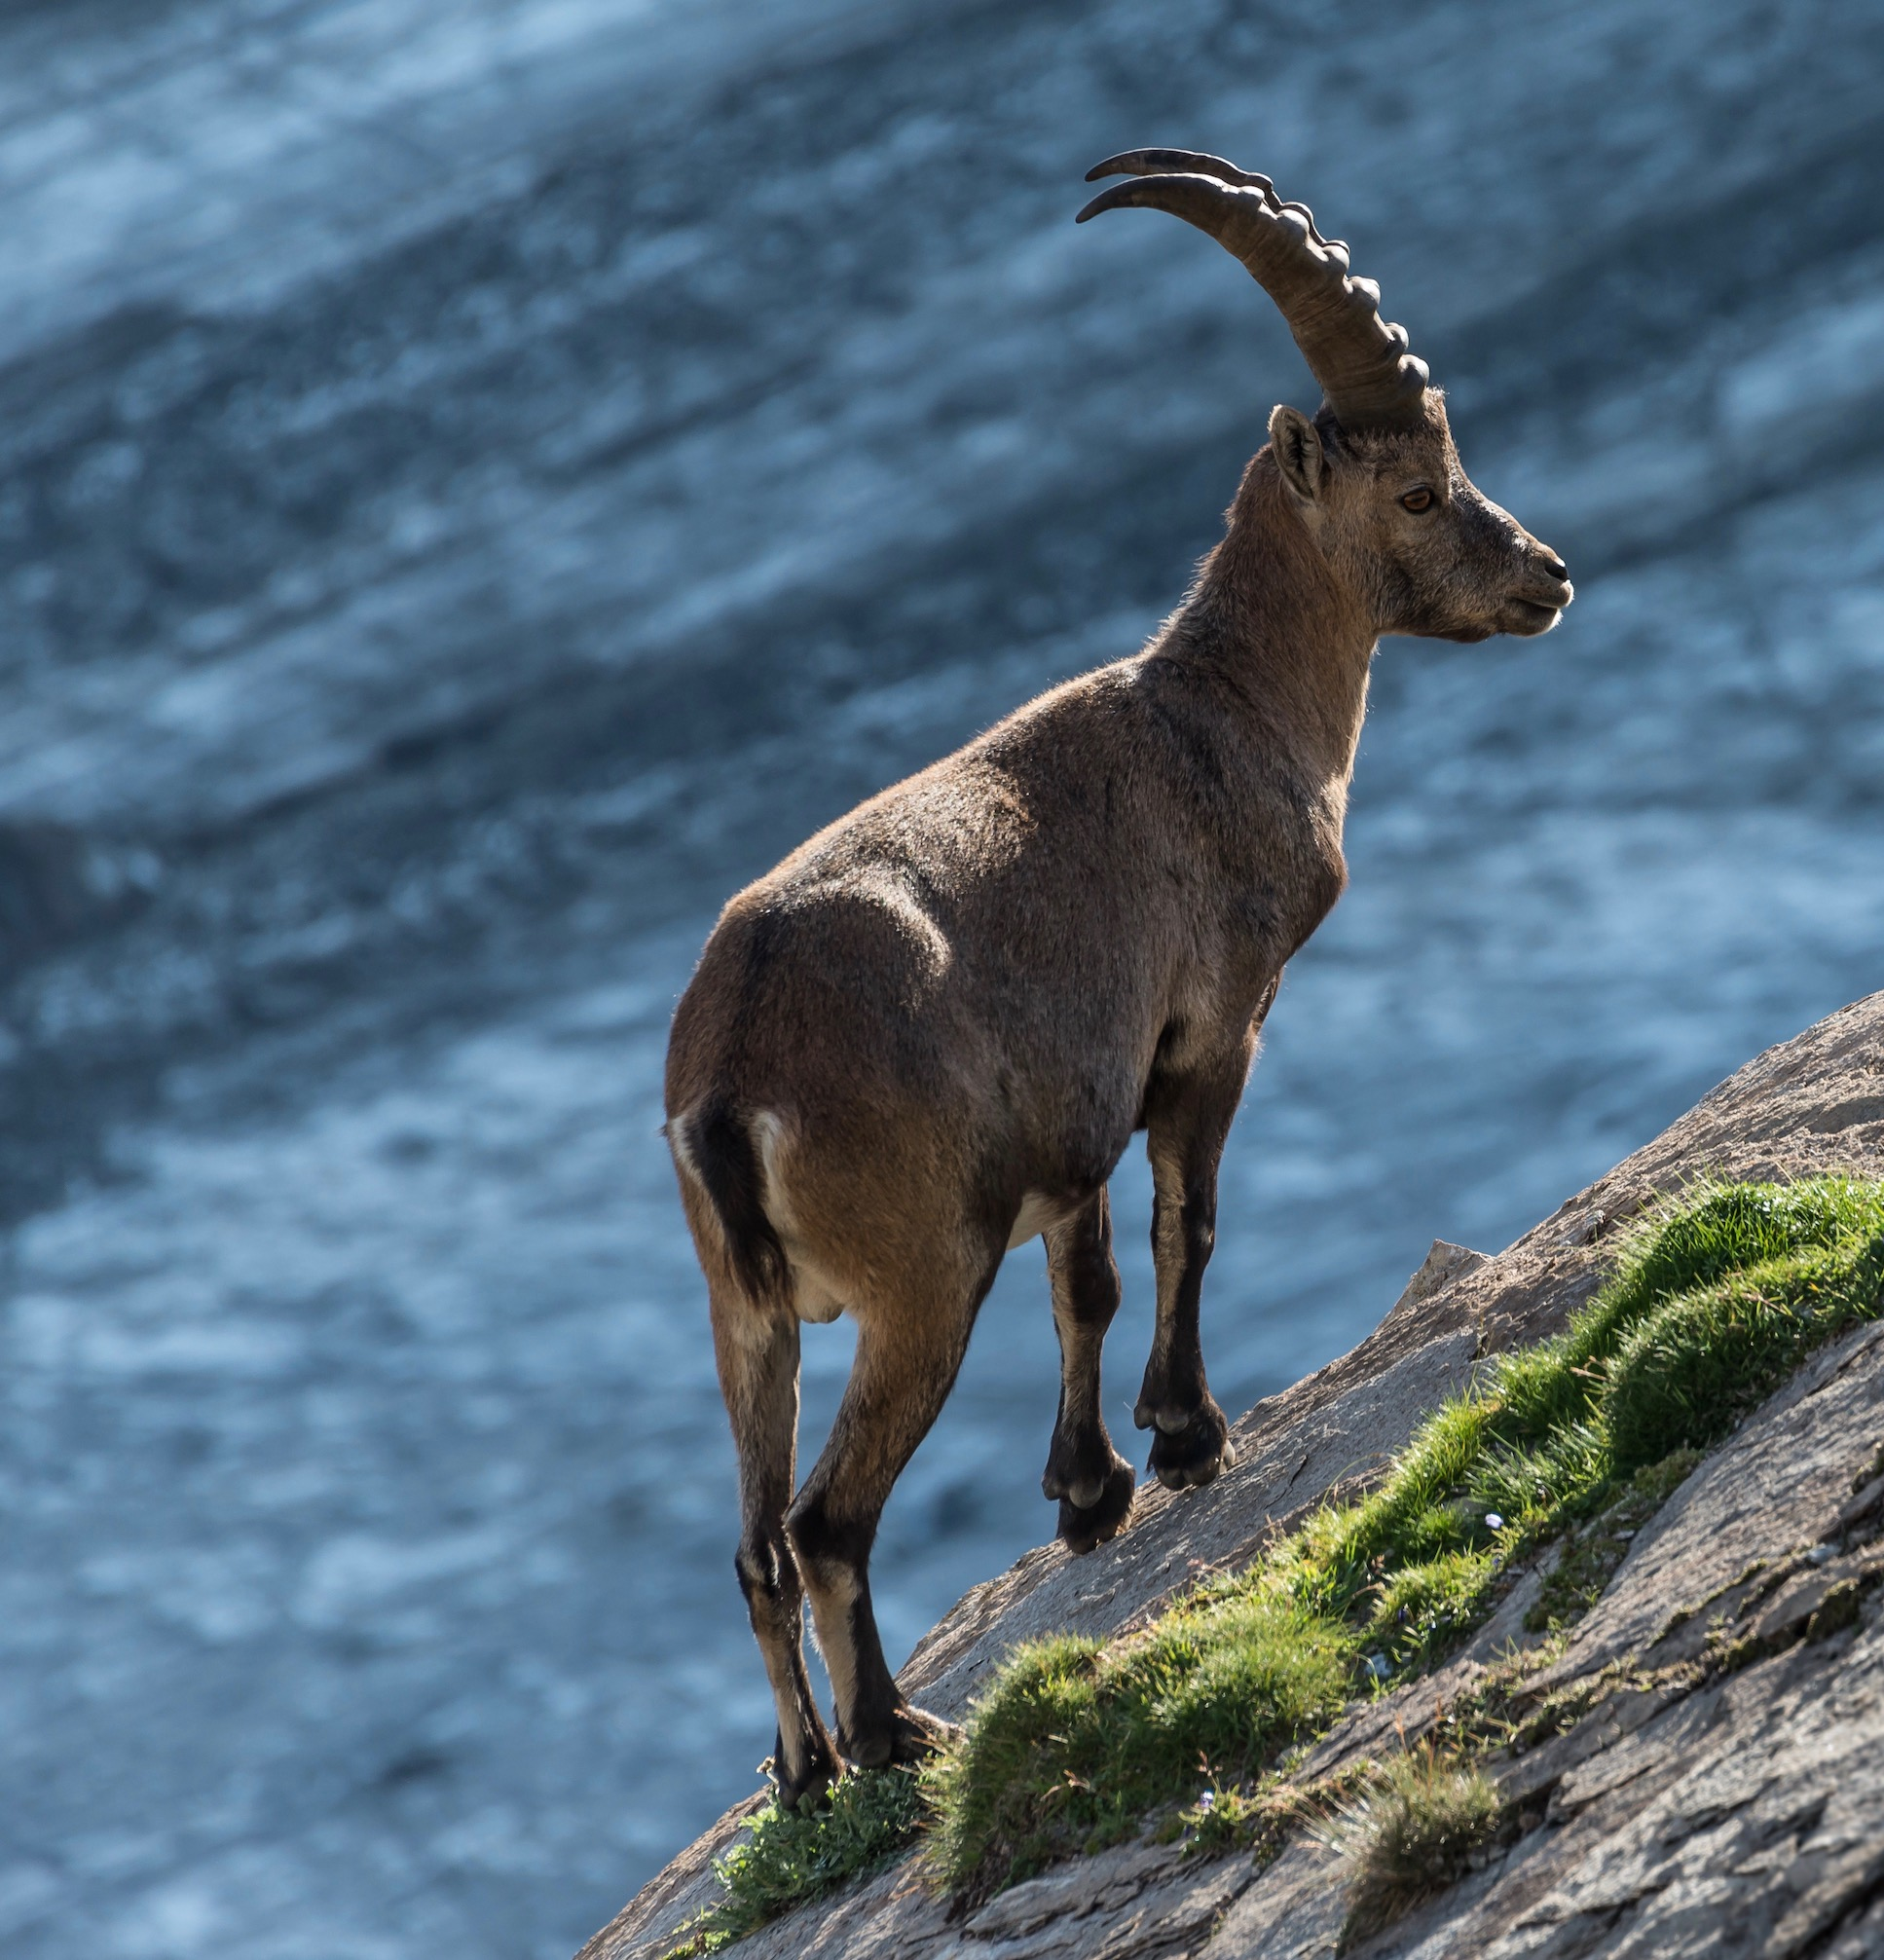
\includegraphics[width=\paperwidth,%
                   keepaspectratio=true]{Steinbock}
\end{textblock*}

%% titre
\begin{textblock*}{2.3\TPHorizModule}(0.35\TPHorizModule,3.5\TPVertModule)
  \pgfsetfillopacity{0.85}
  \textcolor{white}{\titlefmt}
  \pgfsetfillopacity{1}
\end{textblock*}

%% auteur
\begin{textblock*}{2\TPHorizModule}(0.35\TPHorizModule,8.5\TPVertModule)
  \pgfsetfillopacity{0.85}
  \textcolor{white}{\authorfmt}
  \pgfsetfillopacity{1}
\end{textblock*}

\null\cleardoublepage

%%%
%%% Page frontispice
%%%

%% titre
\begin{textblock*}{2.3\TPHorizModule}(0.35\TPHorizModule,3.5\TPVertModule)
  \pgfsetfillopacity{1}       % autrement titre un peu trop haut (?)
  \titlefmt
\end{textblock*}

%% auteur
\begin{textblock*}{2\TPHorizModule}(0.35\TPHorizModule,8.5\TPVertModule)
  \pgfsetfillopacity{1}       % idem
  \authorfmt
\end{textblock*}

%% affiliation
\begin{textblock*}{2\TPHorizModule}(0.35\TPHorizModule,10.5\TPVertModule)
  \affiliation
\end{textblock*}

%% édition
\begin{textblock*}{1.7\TPHorizModule}(0.35\TPHorizModule,30\TPVertModule)
  \edition
\end{textblock*}
\endgroup

%%% Local Variables:
%%% mode: latex
%%% TeX-engine: xetex
%%% TeX-master: "theorie-credibilite-avec-r"
%%% coding: utf-8
%%% End:

\null\cleardoublepage           % cf. section 2.2 textpos.pdf

%%% Copyright (C) 2018 Vincent Goulet
%%%
%%% Ce fichier fait partie du projet
%%% «Théorie de la crédibilité avec R»
%%% http://github.com/vigou3/theorie-credibilite-avec-r
%%%
%%% Cette création est mise à disposition selon le contrat
%%% Attribution-Partage dans les mêmes conditions 4.0
%%% International de Creative Commons.
%%% http://creativecommons.org/licenses/by-sa/4.0/

\begingroup
\calccentering{\unitlength}
\begin{adjustwidth*}{\unitlength}{-\unitlength}
  \setlength{\parindent}{0pt}
  \setlength{\parskip}{\baselineskip}
  \small

  {\textcopyright} {\year} Vincent Goulet \\

  
\includegraphics[height=7mm,keepaspectratio=true]{by-sa}\\%
  Cette création est mise à disposition selon le contrat
  \href{http://creativecommons.org/licenses/by-sa/4.0/deed.fr}{%
    Attribution-Partage dans les mêmes conditions 4.0 International} de
  Creative Commons. En vertu de ce contrat, vous êtes libre de:
  \begin{itemize}
  \item \textbf{partager} --- reproduire, distribuer et communiquer
    l'{\oe}uvre;
  \item \textbf{remixer} --- adapter l'{\oe}uvre;
  \item utiliser cette {\oe}uvre à des fins commerciales.
  \end{itemize}
  Selon les conditions suivantes:

  \begin{tabularx}{\linewidth}{@{}lX@{}}
    \raisebox{-9mm}[0mm][13mm]{%
      
\includegraphics[height=11mm,keepaspectratio=true]{by}} &
    \textbf{Attribution} --- Vous devez créditer l'{\oe}uvre, intégrer
    un lien vers le contrat et indiquer si des modifications ont été
    effectuées à l'{\oe}uvre. Vous devez indiquer ces informations par
    tous les moyens possibles, mais vous ne pouvez suggérer que
    l'Offrant vous soutient ou soutient la façon dont vous avez utilisé
    son {\oe}uvre. \\
    \raisebox{-9mm}{
\includegraphics[height=11mm,keepaspectratio=true]{sa}}
    & \textbf{Partage dans les mêmes conditions} --- Dans le cas où vous
    modifiez, transformez ou créez à partir du matériel composant
    l'{\oe}uvre originale, vous devez diffuser l'{\oe}uvre modifiée dans
    les même conditions, c'est à dire avec le même contrat avec lequel
    l'{\oe}uvre originale a été diffusée.
  \end{tabularx}

  Les exercices sont dérivés de \citet{Cossette:credibilite:2008}, un
  document sous contrat
  \href{http://creativecommons.org/licenses/by-sa/2.5/ca/}{%
    CC BY-SA 2.5 Canada}.

  \textbf{Code source} \\
  \viewsource{\ghurl}

  \textbf{Couverture} \\
  Bouquetin des Alpes (\emph{Capra ibex}) du parc national autrichien du Hohe Tauern.
  Photo: {\textcopyright} Bernd Thaller,
  \href{https://creativecommons.org/licenses/by-sa/3.0/at/deed.en}{CC
    BY-SA 3.0 Autriche}, via
  \href{https://commons.wikimedia.org/w/index.php?curid=40071439}{Wikimedia
    Commons}.
\end{adjustwidth*}
\endgroup

%%% Local Variables:
%%% mode: latex
%%% TeX-engine: xetex
%%% TeX-master: "theorie-credibilite-avec-r"
%%% coding: utf-8
%%% End:

\clearpage

\pagestyle{companion}

%%%% Copyright (C) 2018 Vincent Goulet
%%%
%%% Ce fichier fait partie du projet
%%% «Théorie de la crédibilité avec R»
%%% http://github.com/vigou3/theorie-credibilite-avec-r
%%%
%%% Cette création est mise à disposition selon le contrat
%%% Attribution-Partage dans les mêmes conditions 4.0
%%% International de Creative Commons.
%%% http://creativecommons.org/licenses/by-sa/4.0/

\chapter{Introduction}
\label{chap:introduction}


\tableofcontents*

%% Vignette xkcd.com
\cleartoverso
\thispagestyle{empty}
\begin{vplace}[0.45]
  \centering
  \begin{minipage}{0.9\linewidth}
    \setkeys{Gin}{width=\textwidth}
    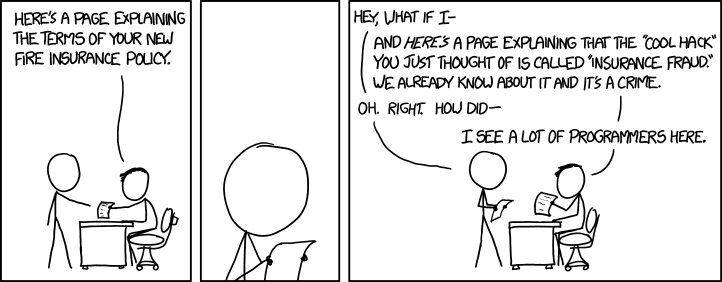
\includegraphics{insurance.png} \\
    \footnotesize\sffamily%
    Tiré de \href{http://xkcd.com/1494/}{XKCD.com}
  \end{minipage}
\end{vplace}

\mainmatter

%%% Copyright (C) 2018 Vincent Goulet
%%%
%%% Ce fichier fait partie du projet
%%% «Théorie de la crédibilité avec R»
%%% http://github.com/vigou3/theorie-credibilite-avec-r
%%%
%%% Cette création est mise à disposition selon le contrat
%%% Attribution-Partage dans les mêmes conditions 4.0
%%% International de Creative Commons.
%%% http://creativecommons.org/licenses/by-sa/4.0/

\chapter{Introduction et perspective historique}
\label{chap:introduction-historique:introduction}

Théorie de la crédibilité: ensemble de techniques utilisées par les
actuaires pour déterminer la prime d'un assuré/contrat dans un
portefeuille hétérogène.

En faisant une tarification, un assureur cherche
\begin{enumerate}
\item d'abord à charger assez de primes pour poyer les sinistres; puis
\item distribuer équitablement ces primes entre les assurés.
\end{enumerate}

Plusieurs façons d'atteindre le second but:
\begin{enumerate}
\item d'abord par une structure de classification; puis
\item par la tarification basée sur l'expérience (\emph{experience
    rating}) $\Rightarrow$ théorie de la crédibilité.
\end{enumerate}

\begin{definition}[\emph{Experience rating}]
  La tarification basée sur l'expérience vise à assigner à chaque
  risque sa prime juste et équitable. Cette prime pour une période
  dépend exclusivement de la distribution des sinistres (inconnue) de
  ce risque pour la période. \citep{Buhlmann:credibility:1969}
\end{definition}

La tarification basée sur l'expérience exige un volume d'expérience
important. Elle est donc principalement utilisée en
\begin{itemize}
\item assurance automobile
\item accidents du travail.
\end{itemize}
Elle ne peut toutefois être utilisée, par exemple, en
\begin{itemize}
\item assurance-vie (on ne meurt qu'une fois)
\item assurance habitation (fréquence trop faible)
\end{itemize}


\section{Illustration des principes de base}
\label{sec:introduction-historique:illustration}

\begin{exemple}
  \label{ex:introduction-historique:simplifie}
  Un portefeuille d'assurance est composé de dix contrats. Les
  contrats sont a priori considérés équivalents. Les conditions
  suivantes prévalent:
  \begin{itemize}
  \item tout contrat ne peut avoir qu'au plus un sinistre par année;
  \item le montant de ce sinistre est $1$;
  \item la prime collective est $0,20$, c'est-à-dire que l'assureur
    s'attend à ce qu'en moyenne deux assurés sur dix aient un sinistre au
    cours d'une année.
  \end{itemize}


\subsection*{Situation après une année}

Voici l'expérience au sein du portefeuille après une année.

\begin{center}
  \begin{tabularx}{\tablewidth}{c*{10}{Y}}
    \toprule
    & \multicolumn{10}{c}{Contrat} \\
    \cmidrule{2-11}
    Année & 1 & 2 & 3 & 4 & 5 & 6 & 7 & 8 & 9 & 10 \\
    \midrule
    $1$ &   &   &   &   &   &   &   &   & 1 &   \\
    \bottomrule
  \end{tabularx}
\end{center}

\begin{itemize}
\item Montant de sinistre moyen par contrat $= 1/10 = 0,10$.
\item La prime collective est \emph{peut-être} trop élevée.
\item Trop peu de données pour tirer une conclusion.
\end{itemize}


\subsection*{Situation après deux années}

Après deux années, l'expérience est maintenant comme suit.

\begin{center}
  \begin{tabularx}{\tablewidth}{c*{10}{Y}}
    \toprule
    & \multicolumn{10}{c}{Contrat} \\
    \cmidrule{2-11}
    Année & 1 & 2 & 3 & 4 & 5 & 6 & 7 & 8 & 9 & 10 \\
    \midrule
    $1$ &   &   &   &   &   &   &   &   & 1 &   \\
    \midrule
    $2$ & 1 & 1 &   &   &   &   &   &   & 1 &   \\
    \bottomrule
  \end{tabularx}
\end{center}

\begin{itemize}
\item Montant de sinistre moyen par contrat $= 4/20 = 0,20$.
\item La prime collective est adéquate.
\item Le contrat $9$ a déjà eu deux sinistres.
\end{itemize}


\subsection*{Situation après dix années}

Observons maintenant la situation après dix années.

\begin{center}
  \begin{tabularx}{\tablewidth}{c*{10}{Y}}
    \toprule
    & \multicolumn{10}{c}{Contrat} \\
    \cmidrule{2-11}
    Année & 1 & 2 & 3 & 4 & 5 & 6 & 7 & 8 & 9 & 10 \\
    \midrule
    $1$ &   &   &   &   &   &   &   &   & 1 &   \\
    \midrule
    $2$ & 1 & 1 & 1 &   &   &   &   &   & 1 &   \\
    \midrule
    $3$ & 1 &   &   &   &   &   &   &   & 1 &   \\
    \midrule
    $4$ &   &   & 1 &   &   &   &   &   & 1 &   \\
    \midrule
    $5$ &   &   &   &   &   &   &   &   & 1 &   \\
    \midrule
    $6$ &   & 1 &   &   &   &   &   &   &   &   \\
    \midrule
    $7$ & 1 & 1 &   & 1 & 1 &   &   &   &   &   \\
    \midrule
    $8$ & 1 &   &   & 1 &   & 1 &   &   & 1 &   \\
    \midrule
    $9$ & 1 &   &   &   & 1 &   &   &   &   &   \\
    \midrule
    $10$ & 1 &   &   &   &   &   &   &   & 1 &   \\
    \midrule
    $\bar{S}_i$ & 0,6 & 0,3 & 0,2 & 0,2 & 0,2 & 0,1 & 0 & 0 & 0,7 & 0 \\
    \midrule
    $\bar{S}$ & \multicolumn{10}{c}{0,23} \\
    \bottomrule
  \end{tabularx}
\end{center}

\begin{itemize}
\item Montant de sinistre moyen par contrat $= 23/100 = 0,23$.
\item La prime collective est raisonnablement adéquate.
\item Le contrat $9$, avec ses sept sinistres, est en effet plus risqué.
\item Les contrats $7$, $8$ et $10$ n'ont eu aucun sinistre.
\end{itemize}



\subsection*{Conclusions}

\begin{itemize}
\item La prime collective, si elle est globalement \emph{adéquate},
  n'est en revanche clairement pas \emph{équitable}.
\item Contrairement à l'hypothèse de départ de l'assureur, le
  portefeuille est \emph{hétérogène}.
\item Besoin d'une technique de tarification basée sur l'expérience
  (\emph{experience rating}) pour adéquatement distribuer les primes
  entre les assurés.
\end{itemize}
  \qed
\end{exemple}

Deux grandes branches en théorie de la crédibilité:
\begin{enumerate}
\item Credibilité de stabilité, ou américaine, \emph{limited
    fluctuations}.

  L'assureur tient compte de l'expérience individuelle seulement si
  celle-ci est suffisamment stable dans le temps.

\item Crédibilité de précision, ou européenne, \emph{greatest
    accuracy}.

  L'assureur tient compte de l'expérience individuelle de façon à
  obtenir la meilleure estimation de l'expérience future. Le poids de
  l'expérience individuelle augmente avec l'hétérogénéité du
  portefeuille.
\end{enumerate}


\section{Historique et évolution de la théorie de la crédibilité}
\label{sec:introduction-historique:historique}

\begin{quote}
  \itshape Cette section reprend une partie du chapitre 1 de
  \cite{Goulet:masters}.
\end{quote}

La personne qui mentionne qu'elle étudie «la crédibilité» obtient
habituellement de grands yeux incrédules et interrogateurs comme seule
réponse de la part de son interlocuteur, fut-il même parfois actuaire.
Pour l'actuaire la crédibilité n'est souvent qu'un vague concept parmi
tant d'autres rencontrés au fil des examens professionnels, concept
qui eut tôt fait de fuir à toutes jambes sa mémoire une fois l'examen
réussi. Quant au non actuaire, l'étude de la crédibilité ne lui
apparaît d'aucun intérêt puisqu'il n'applique habituellement la notion
qu'aux personnes physiques: le juge est crédible lorsqu'il interprète
la loi, certains critiques de cinéma sont crédibles alors que d'autres
le sont moins, nul politicien n'est considéré crédible... Pourtant, la
définition que donne le \emph{Petit Robert} du mot crédibilité, «ce
qui fait qu'une chose mérite d'être crue; caractère de ce qui est
croyable», est assez vaste pour laisser place à d'autres
interprétations.

La population accorde donc de la crédibilité aux gens, et ce selon
leur notoriété, leurs réalisations, du fait d'expériences concluantes,
de leur honnêteté et leur droiture reconnues ou tout simplement par
affinité. En fin de compte, une personne est crédible à nos yeux s'il
est \emph{probable} que ce qu'elle dit ou fait se réalise ou soit un
succès. Par exemple, il est fort probable que l'interprétation que le
juge fait de la loi soit la bonne; ou j'irai voir le nouveau film à
l'affiche louangé par tel critique car je sais qu'il est probable que
je l'aime moi aussi.

On voit donc qu'il existe une étroite relation entre les notions de
«probabilité» et de «crédibilité». C'est pour cette raison qu'avant
d'aborder l'historique de la théorie actuarielle de la crédibilité, il
s'avérera intéressant d'étudier l'évolution de l'approche probabiliste
privilégiée en actuariat, l'approche bayésienne. Avec en plus l'étude
des réflexions sur le sujet du philosophe anglais Bertrand Russell le
lien entre les deux notions se clarifiera et la perspective historique
n'en sera que meilleure.

\subsection{L'émergence de l'approche bayésienne}

Bien que Thomas Bayes eut présenté son fameux théorème dans un essai
en 1763, ce n'est que dans la seconde moitié des années 1950 que la
philosophie probabiliste basée sur ce théorème gagne suffisamment
d'adeptes, et donc de popularité, pour aspirer au respect. L'approche
classique monopolisait auparavant la foi des probabilistes et
statisticiens, et c'est encore aujourd'hui la philosophie enseignée en
premier lieu dans les écoles.

Le statisticien classique%
\footnote{Souvent appelé \emph{objectivist} en anglais. L'expression
  est toutefois difficile à traduire adéquatement en français et c'est
  pourquoi usage on utilisera le terme «classique»} %
a une vision très stricte, objective et mathématique de la probabilité
et de l'usage qu'il est possible d'en faire pour inférer un résultat à
partir de données. Pour lui, une probabilité est essentiellement la
limite d'une série de fréquences relatives où la symétrie joue un rôle
primordial: si un événement peut connaître $n$ réalisations
différentes mutuellement exclusives et ayant une chance égale de se
réaliser, et si de ces réalisations $m$ ont l'attribut $A$, alors la
probabilité de $A$ est $m/n$. Des énoncés du type «il est probable que
le Québec devienne indépendant au cours des deux prochaines années» ou
«il est probable qu'il neige demain» n'ont donc aucun sens à ses yeux.
D'ailleurs, les statisticiens classiques croient que leur travail se
limite exclusivement à l'analyse des données et qu'il ne leur
appartient pas de prendre des décisions à la lumière des résultats
obtenus. Il sera expliqué plus loin que, par opposition, les bayésiens
voient en la prise de décision le but de tout travail statistique.

Un autre élément majeur qui caractérise l'approche classique --- et
c'est celui qui concerne particulièrement la théorie de la crédibilité
--- est l'absence de prise en compte de toute information a priori
relative au problème étudié. On préfère «laisser les données parler
d'elles-mêmes». C'est ce qui fut à l'origine de la contestation devant
mener à l'émergence de l'approche bayésienne.

Leonard J.\ Savage publie en 1954 \citep{Savage:foundations:1954} un des premiers
livres consacrés à l'étude de la statistique dans une optique
bayésienne. Il défend alors la vision individualiste de la probabilité
(\emph{personalistic view of probability}) qu'il qualifie de «seul
concept de probabilité». Comme son nom l'indique, cette vision tâche
de se rapprocher le plus possible du raisonnement humain.  La
probabilité devient donc un indicateur de l'opinion d'une personne à
propos d'un événement et, puisqu'une opinion est --- habituellement!
--- sujette à changement suite à l'ajout d'informations, l'inférence
statistique à partir de nouvelles données constitue alors le mécanisme
de révision de l'opinion. De plus, l'adhérant à cette vision refuse
obstinément de rejeter toute information parallèle ou a priori au
problème sous prétexte que, justement, l'humain tire profit de ces
informations lorsqu'il prend une décision. Si la question «quel degré
de conviction puis-je atteindre à la suite de l'ajout de cette information?»
est hors du champ de la statistique pour le statisticien classique,
elle est au contraire au c{\oe}ur même du problème pour
l'individualiste.  Ce dernier répond d'ailleurs à la question en
utilisant le théorème de Bayes --- d'où le qualificatif de bayésien.
Cet algorithme donne la nouvelle probabilité d'un événement $A$ à
partir de sa probabilité originale et des nouveaux faits marquants
venant s'y rattacher. Ainsi, si $B$ constitue l'ensemble des nouveaux
faits, alors
\begin{equation*}
  P[A|B]= \frac{P[B|A]P[A]}{P[B]},
\end{equation*}
où $P[A]$ est la probabilité a priori que l'événement $A$ se réalise.

De plus, les bayésiens évitent l'apparente contradiction entre
l'objectivité scientifique et l'irrationalité humaine en postulant un
individu idéal, conséquent dans ses décisions. Par exemple, cet
individu, lorsque confronté à un choix, choisira toujours l'option la
plus probable.

Savage donne dans son ouvrage \emph{The foundations of statistics}
quelques expressions synonymes pour \emph{personal probability}:
\emph{subjective probability}, \emph{psychological probability} et,
finalement, \emph{degree of conviction}. Le lecteur est invité à
conserver tout particulièrement en mémoire la dernière expression. En
effet, la section suivante étudie sommairement les travaux du
philosophe Bertrand Russell et il sera intéressant de constater à quel
point les travaux de deux disciplines différentes ont su converger.

\subsubsection{Les réflexions de Russell}

Lord Bertrand Russell (1872-1970) est un éminent philosophe et
logicien britannique, pacifiste invétéré et dont l'activité la plus
marquante se rapporta aux mathématiques et à la logique. Il est entre
autres le fondateur du logicisme, doctrine selon laquelle «les
mathématiques seraient soumises à la formalisation de la logique et
s'y réduiraient» (\emph{Le Petit Larousse}). Il fut récipiendaire du
Prix Nobel de littérature en 1950.

Joseph Butler (1692--1752) disait: «la probabilité est le guide de la
vie d'une personne».  En effet, il est raisonnable de croire que
lorsque deux événements ou plus ont des chances de se réaliser, la
décision d'une personne sera basée sur celui qui se réalisera avec la
plus forte probabilité. Mais ce type de probabilité est-il le même que
dans l'énoncé: «la probabilité d'obtenir un double six au lancer de
deux dés est de un sur trente-six»? Russell soutient que non. Voici
son raisonnement, que l'ont peut retrouver de façon plus exhaustive
dans son ouvrage de 1948 \citep{Russell:human:1948}.

De toute évidence, cette dernière est la probabilité dite
\emph{mathématique}, obéissant aux axiomes de la théorie des
probabilités, que l'on peut grossièrement réduire au quotient de deux
nombres: le cardinal d'une classe spécifique (double six) et celui
d'une classe fondamentale (les réalisations possibles du lancer de
deux dés). Elle s'attarde aux énoncés d'ordre général, se référant à
des classes «anonymes». Un autre exemple serait, en assurance-vie: «la
probabilité qu'un homme non-fumeur âgé de 30 ans décède dans l'année
qui vient est, selon la table CSO 1958, de $0,00213$». Jamais dans ces
deux exemples il n'est fait référence à une personne ou un objet en
particulier.

Cependant, en passant à un cas particulier du genre «la probabilité
que je vive jusqu'à 90 ans est de $60~\%$», est-on toujours dans le
domaine de la probabilité mathématique? Au passage d'un cas général à
un cas particulier (et en ne considérant pas le cas particulier comme
une simple réalisation du phénomène général), une personne devrait
être en mesure d'intégrer \emph{tous} les éléments d'importance à sa
prise de décision. Cette masse d'information lui permettrait alors de
savoir avec certitude si oui ou non sa longévité atteindra les 90 ans.
Et dès lors elle se retrouverait hors du champ de la probabilité.

Bien entendu, il est pour ainsi dire impossible d'atteindre un tel
niveau de certitude. C'est pourquoi la probabilité demeure le guide de
la vie de la personne, parce que \emph{son savoir s'avère
  insuffisant}. Mais encore, si ce guide est la probabilité
mathématique, il doit être possible de calculer et d'identifier
\emph{la} probabilité (c'est-à-dire \emph{la} classe fondamentale),
sinon le guide fait faux bon à son utilisateur! La personne en quête
de cette probabilité évaluera donc d'abord elle-même ses chances de
vivre jusqu'à 90 ans, puis ira probablement consulter un médecin, ou
même une voyante, qui chacun lui donnera son avis, pas nécessairement
objectif. Cette personne ne pourra que croire en totalité ou en partie
les divers jugements colligés, aussi lorsqu'il affirmera «la
probabilité que je vive jusqu'à 90 ans est de $60~\%$», il attribuera
en réalité une \emph{crédibilité} de $60~\%$ à l'expression «je vais
vivre jusqu'à 90 ans». C'est le mieux qu'il pourra faire, tout le
savoir de l'humain comportant une part de doute ou, à
l'inverse, seulement un \emph{degré de crédibilité}.

Crédibilité, voilà donc le nom qu'attribue Russell à ce second type de
probabilité, la distinction entre la probabilité mathématique et la
crédibilité se faisait au \emph{passage du général au particulier}.
Une relation subsiste néanmoins entre les deux notions, et c'est que
la probabilité mathématique est un instrument de mesure de la
crédibilité. De plus, toujours selon Russell, tout énoncé comporte un
degré de crédibilité intrinsèque, si minime soit-il, car une personne
a toujours un certain bagage de connaissances lui permettant de se
faire une opinion a priori. Finalement, la crédibilité peut être
augmentée par l'ajout d'information, le gain marginal allant en
décroissant.

Cette théorie de Bertrand Russell date de 1948 (ou du moins sa
publication). L'énoncé sommaire ci-dessus suffit pour constater à quel
point cette théorie est près de l'approche bayésienne en statistique
qui commençait alors à sortir de l'anonymat. Cela n'est pas surprenant
si l'on se rappelle que les fondateurs de l'école bayésienne ont,
comme des philosophes le font, basé leur théorie sur le comportement
humain. Ainsi, ce que Russell nomme probabilité mathématique correspond
en fait à l'approche classique en statistique et il ne la considère
pas comme un fin en soi, mais bien comme un outil pour une prise de
décision. C'est cette prise de décision, via la détermination d'un
degré de crédibilité, qui constitue la fin de l'utilisation de la
probabilité (ou de la statistique). D'ailleurs, l'expression
\emph{degree of conviction} proposée par Savage n'est-elle pas
synonyme de celle de Russell, degré de crédibilité?

Cependant, là où le philosophe fortifie le plus la thèse bayésienne,
c'est lorsqu'il soutient que tout énoncé comporte un degré de
crédibilité intrinsèque car, ce faisant, il défend l'apport non
négligeable de l'information a priori.

\subsection{Et les actuaires dans tout ça?}

Longtemps avant l'apparition de l'approche bayésienne ou même les
théories de Russell, l'information a priori était prise en compte par
les actuaires. En effet, lorsqu'ils évaluaient une prime, jamais ils
n'auraient considéré ne \emph{rien} connaître du risque. À partir de
différents critères, ils arrivaient au moins à le regrouper avec
d'autres risques semblables. Toutefois, le mécanisme de prise en
compte de cette information était souvent ad hoc et mal compris à
la fois par les actuaires et les statisticiens. C'était la
crédibilité.

Si la crédibilité a su se développer et faire le bonheur de ses
utilisateurs pendant de nombreuses années sans les bases statistiques
de l'approche bayésienne, il n'en demeure pas moins que l'arrivée de
celle-ci marqua un virage important dans l'évolution de la
crédibilité, contribuant d'ailleurs à en faire davantage une théorie.
Les lignes suivantes tâcheront de retracer l'évolution historique de
la théorie de la crédibilité, de ses balbutiements aux débuts du
siècle à son adolescence actuelle, tout en faisant le lien avec les
théories présentées plus haut.

La petite histoire suivante, inventée par le Dr François Dufresne pour
un cours d'introduction à la théorie de la crédibilité à l'Université
Laval, illustre sans doute bien comment cette théorie a pu voir le
jour.

Vers les années 1910, aux États-Unis, la multinationale General Motors
et le petit constructeur indépendant Tucker sont assurés chez Allstate
contre les accidents de travail (\emph{workers compensation}), avec
quelques autres fabricants d'automobiles. Un taux moyen est calculé à
partir de l'expérience de l'ensemble de ces fabricants et c'est ce
taux qui est chargé à chacun. Or, la GM calcule elle-même son taux et
s'aperçoit qu'il serait, année après année, inférieur à celui qu'on
lui charge et ce, grâce à une expérience meilleure que celle du
groupe. Exaspérée par une telle situation, elle demande à Allstate
qu'on lui charge son propre taux, ceci sous prétexte que son nombre
d'employés important est un gage de stabilité de l'expérience entre
les années.

Les actuaires de Allstate sont intuitivement d'accord avec
l'argumentation de GM, aussi s'apprêtent-ils à accéder à sa demande.
Un petit problème les fait cependant hésiter: si le nombre d'employés
de GM est clairement assez gros pour que l'on se fie à son expérience
et celui de Tucker trop petit pour faire de même, où fixera-t-on la
limite entre un nombre d'employés fiable et un non fiable?

Il est généralement reconnu que le premier actuaire à avoir proposé
une solution au problème dans la littérature est Arthur H.\ Mowbray,
dans le premier numéro des Proceedings de la Casualty Actuarial
Society, en 1914 \citep{Mowbray:1914}. En supposant connue la
probabilité $q$ qu'un accident survienne, il désire calculer le nombre
minimal d'employés assurés $n$ de telle sorte que la probabilité que
le nombre d'accidents ne s'éloigne pas de plus de $100k$~\% de la
moyenne (ou du mode%
\footnote{Mowbray privilégie la valeur la plus fréquente, le mode,
  mais s'en remet à la moyenne par simplicité et sous prétexte que ces
  deux valeurs sont presque égales.}) %
soit supérieure à $100p$~\%. Si l'on note $N$ la distribution du
nombre d'accidents, alors l'énoncé précédent s'écrit en langage
mathématique
\begin{equation*}
  P \left[ (1 - k)E[N] \leq N \leq (1 + k)E[N] \right] \geq p,
\end{equation*}
où $N \sim \text{Binomiale}(n, q)$. Par la suite, l'utilisation de
l'approximation normale pour la distribution de $N$ permet d'éviter
l'arbitrage entre le mode et la moyenne et d'obtenir aisément une
réponse.

Les bases de la crédibilité de stabilité, ou \emph{limited
  fluctuations}, étaient dès lors posées.

La solution de Mowbray était intéressante car appuyée par des
arguments probabilistes. Elle connut d'ailleurs de multiples
adaptations qui lui permirent de rester d'actualité jusqu'à nos jours.
Moyennant la détermination d'une distribution pour le nombre de
sinistres, les praticiens pouvaient désormais résoudre par un calcul
simple le problème auquel ils faisaient face: fixer un seuil
d'admissibilité à la pleine crédibilité.

Les assurés eurent cependant tôt fait de soumettre un autre problème
aux actuaires. Telle que présentée jusqu'à maintenant, la théorie de
la crédibilité n'admettait que deux niveaux: $0$ et $1$. Or, cette
situation pouvait se traduire, pour un employeur situé tout juste sous
le seuil d'admissibilité, en une différence significative dans la
prime à payer. De plus, la notion même de pleine crédibilité ne
ralliait pas l'ensemble des actuaires, certains croyant que jamais les
données ne sont fiables à $100~\%$.

C'est pour répondre à ces critiques que fut introduit le concept de
crédibilité partielle, dont on attribue la première véritable théorie
sur le sujet à \cite{Whitney:1918}. Dès 1918 donc, Whitney mentionne la
«nécessité, par souci d'équité pour l'assuré, de pondérer d'un côté
l'expérience collective et de l'autre l'expérience individuelle».
L'essence de la crédibilité consistait à calculer cette pondération.

À au moins deux reprises dans l'histoire, la crédibilité de précision
(\emph{greatest accuracy}) a eu la chance de s'imposer avant la
contribution de Bühlmann en 1967. La première se trouve dans les
travaux de Whitney. Dans son article, ce dernier retient quatre
éléments qui influenceront la pondération à donner à l'expérience
individuelle: l'exposition, le niveau de risque, la crédibilité de la
prime collective et l'homogénéité du groupe. D'ailleurs, il mentionne:

\begin{quote}
  «Il n'y aurait pas de problème d'\emph{experience rating} si chaque
  risque dans le groupe était typique du groupe, car dans ce cas les
  variations dans l'expérience ne seraient que purement aléatoires.»
  (Traduction libre)
\end{quote}

Or, la notion d'homogénéité du collectif est au c{\oe}ur même de la
crédibilité de précision. Whitney modélise l'hétérogénéité du
collectif en supposant que les moyennes des divers risques sont
distribuées selon une loi normale. De là, par un développement
mathématique lourd et laborieux, il obtient une expression pour la
prime individuelle ($P$) de la forme
\begin{equation*}
  P = z X + (1 - z) C,
\end{equation*}
où $X$ est l'expérience individuelle et $C$, l'expérience collective.
Ces valeurs sont pondérées par le facteur de crédibilité, $z$, dont
Whitney obtient une formule de la forme $n/(n + K)$. $K$ n'est alors
pas une constante arbitraire, mais bien une expression explicite
dépendant des divers paramètres du modèle. Par souci de simplicité,
Whitney suggère cependant de fixer $K$ comme une constante à
déterminer au jugement de manière à éviter les trop grandes
fluctuations entre la prime individuelle et la prime collective. Ce
faisant, il s'écarte d'une conception de la crédibilité visant la
précision pour encourager plutôt celle visant la stabilité. La
crédibilité de précision meurt dans l'{\oe}uf à cause de
considérations d'ordre pratique.

Whitney fut de plus critiqué par \cite{Fisher:Whitney:discussion:1919}
pour avoir utilisé une méthode jugée hérétique à l'époque en
statistique, la règle de Bayes. Fisher cite d'ailleurs quelques
personnes faisant autorité s'étant prononcées contre l'usage de cette
règle. En fait, Whitney utilise la version la plus simple de la règle,
celle même proposée par Bayes\footnote{%
  Selon \cite{Bailey:1950}.}, %
qui suppose qu'a priori tous les événements ont une chance égale de se
réaliser. Cette modélisation était appelée par ses adeptes le
«Principe de la raison insuffisante» et par ses détracteurs
«L'hypothèse de distribution uniforme de l'ignorance»%
\footnote{\emph{Principe of insufficient reason} et \emph{Assumption
    of the equal distribution of ignorance.}}. %
Dans le développement de Whitney, cela revient à supposer que toutes
les valeurs possibles pour la moyenne du groupe sont équiprobables.
Les réserves de Fisher sur ce point étaient donc justifiées...

Il est difficile aujourd'hui de mesurer l'impact que la volte-face de
Whitney en faveur des arguments de stabilité a pu avoir sur la
pratique de la crédibilité. Toujours est-il que les actuaires ont
utilisé intensivement pendant un demi-siècle la forme $z = n/(n + K)$ pour
calculer des facteurs de crédibilité basés essentiellement sur la
stabilité. Encore aujourd'hui, c'est l'approche privilégiée aux
États-Unis. Pourtant, si les pratiques se sont quelque peu figées, la
théorie, elle, n'a pas cessé d'évoluer.

L'approche de précision tente à nouveau sa chance par l'entremise de
Arthur L.~Bailey, et ce à deux reprises (\cite{Bailey:1945} et
\cite{Bailey:1950}). En 1945 d'abord, Bailey obtient une expression pour
la crédibilité dans ce qui semble être l'univers non paramétrique
exploré plus tard par Bühlmann. Seulement, une notation confuse rend
le texte difficilement déchiffrable et le condamne à la marginalité.

L'article de 1950 avait, lui, davantage le potentiel pour ébranler les
acquis en théorie de la crédibilité. Bailey débute son article en
relevant les confrontations historiques entre statisticiens et
actuaires au sujet de la crédibilité. On apprend alors qu'il y a plus
de trente ans, la polémique au sujet de la crédibilité était la même
que de nos jours: les statisticiens «purs» crient au scandale,
estimant les méthodes actuarielles contraires à toute théorie
statistique, et les actuaires leur répondent que «peut-être, mais ça
fonctionne!» Le point majeur de discorde est l'utilisation par les
actuaires de la règle de Bayes. Ainsi, \cite{Bailey:1950} écrit:

\begin{quote}
  «Présentement, presque toutes les méthodes d'estimation présentées
  dans les livres de méthode statistiques ou enseignées dans les
  universités américaines sont basées sur un équivalent de l'hypothèse
  selon laquelle toute information parallèle ou connaissance a priori
  est inutile. (...) Des philosophes [Russell] ont récemment étudié la
  crédibilité à accorder à divers éléments de savoir, remettant par
  conséquent en doute la philosophie adoptée par les statisticiens.
  Par contre, il semble que ce ne soit que dans le domaine de
  l'actuariat qu'on ait assisté à une réelle révolte contre la mise de
  côté de tout savoir a priori au moment d'estimer une quantité à
  l'aide de nouvelles données.» (Traduction libre)
\end{quote}

Bailey se prononce donc clairement en faveur de la philosophie
bayésienne. Il semble même qu'il fut le premier à en défendre si
énergiquement la pertinence dans le processus de tarification. Mais
ceci, fait-il remarquer, à condition d'utiliser une généralisation de
la règle de Bayes, faite par Laplace en 1820, de manière à éviter le
controversé «Principe de la raison insuffisante». Cette généralisation
rend la règle de Bayes applicable même si les événements n'ont pas a
priori une chance égale de se réaliser.

À partir de ces prémisses, Bailey démontre qu'en minimisant l'erreur
quadratique dans un contexte bayésien, l'estimateur obtenu est une
fonction linéaire des observations%
\footnote{De la forme $c_0 + \sum_{i,j} c_{ij} X_{ij}$.} %
qui correspond exactement à la prime de crédibilité, et ce pour les
combinaisons de distributions binomiale/bêta, Poisson/gamma et
normale/normale. Il est possible d'en déduire un facteur de
crédibilité encore une fois de la forme $z = n/(n + K)$ où $K$ est une
combinaison des paramètres du modèle.  Contrairement à Whitney, Bailey
ne propose pas d'évaluer $K$ au jugement, mais bien de s'en tenir à
l'expression développée algébriquement.

De plus, conscient que la procédure utilisée est une modélisation de
l'hétérogénéité d'un groupe, Bailey mentionne pour la première fois
que la crédibilité pourrait être utilisée hors du domaine de
l'assurance générale. Malheureusement pour Bailey, le manque de
popularité de l'approche bayésienne au sein de la communauté
statistique au moment de la parution reléguera son article dans
l'ombre. Sans doute l'approche très «théorique» de l'article, publié
dans une revue essentiellement de praticiens, aura-t-elle aussi
contribué à cet état de fait. Pourtant, dans un avenir pas si
lointain, les travaux de Bailey seront reconnus pour leur importance
et leur avant-gardisme. Cette reconnaissance proviendra cependant
majoritairement d'outre-Atlantique.

L'apport de Bailey à la théorie de la crédibilité peut être résumé en
deux points principaux: l'introduction explicite du principe de Bayes
dans le processus de tarification et la découverte de la linéarité de
l'estimateur bayésien sous certaines conditions%
\footnote{Sur ce point toutefois, il est difficile de savoir qui fut
  le pionnier. \cite{Norberg:credibility:1979} relève que
  \cite{Keffer:1929} a obtenu le même résultat pour le modèle
  Poisson/gamma. Toujours selon Norberg, il existerait aussi des
  références antérieures à 1929.} %
Ces développements parvinrent aux oreilles de la communauté
actuarielle européenne par la bouche de Bruno de~Finetti au colloque
ASTIN à Trieste, en 1963. Depuis quelques années déjà, les
chercheurs européens tâchaient de trouver une justification théorique
à ces formules de crédibilité américaines qui fonctionnaient si bien.
L'approche bayésienne avait là aussi fait des progrès importants,
notamment grâce à Bruno de~Finetti dans les années 1930 et Ove Lundberg
dans les années 1940.

Parallèlement à tout cela, une nouvelle branche de la théorie
bayésienne voyait le jour sous l'initiative de Herbert Robbins:
l'approche bayésienne empirique. Celle-ci sera d'une importance
capitale dans le développement futur de la crédibilité de précision
puisqu'elle lui permettra de sauter le mur entre la théorie et la
pratique. L'approche bayésienne empirique
\citep{Robbins:empiricalbayes:1955,Robbins:empiricalbayes:1964}
s'attaque au principal problème pratique de l'approche bayésienne
pure, soit la fréquente ignorance de la distribution a priori.
Jusqu'alors, lorsqu'une telle situation se présentait, il était
coutume d'éviter le problème en réfutant l'aspect aléatoire d'une
partie de la décision \citep{Neyman:1962}. Grossièrement, la thèse de
Robbins consiste à supposer que, bien qu'elle soit inconnue, la
distribution a priori existe et qu'il est possible de l'estimer --- ne
serait-ce qu'indirectement --- à partir de données issues de plusieurs
expériences similaires. Selon lui \citep{Robbins:empiricalbayes:1964}:
\begin{quote}
  «L'approche bayésienne empirique de problèmes statistiques de prise
  de décision est applicable lorsque la même décision se présente à
  répétition et indépendamment avec une distribution fixe, mais
  inconnue du paramètre.» (Traduction libre)
\end{quote}

Comme devait plus tard le mentionner Bühlmann, cela cadre
admirablement bien avec le problème de l'\emph{experience rating}.

Tous ces éléments --- les travaux de Bailey, la popularité
grandissante des approches bayésienne et bayésienne empirique ---
étaient réunis lors du congrès ASTIN de 1965, à Lucerne. Hans
Bühlmann y redéfinit alors le problème fondamental en \emph{experience
  rating} et présente la solution qui allait révolutionner la théorie
de la crédibilité. En forçant la prime bayésienne à être linéaire,
Bühlmann (1967, 1969) obtient, dans un cadre non paramétrique, un
facteur de crédibilité de la forme $z = n/(n+K)$, avec une expression
simple et générale pour $K$. Le virage sera alors définitivement pris
en faveur de l'approche de précision et l'essentiel de la recherche se
fera en Europe. C'est pourquoi l'approche traitant l'hétérogénéité est
aujourd'hui souvent appelée «crédibilité européenne» malgré qu'elle
origine des États-Unis (notamment dans les travaux de Bailey).
L'approche de stabilité, \emph{limited fluctuations}, a par conséquent
reçu l'appellation «crédibilité américaine».

On peut sans crainte poser que le célèbre modèle de Bühlmann
marque le début de l'histoire contemporaine de la théorie de la
crédibilité. Celle-ci étant bien davantage documentée et connue, on va
maintenant se contenter de présenter chronologiquement les principaux
modèles qui suivirent celui de Bühlmann%
\footnote{La liste ne comporte que les principaux modèles et n'est
  donc en rien exhaustive.}. %
La plupart de ces modèles se veulent des généralisations, de plus en
plus poussées, du modèle original de Bühlmann et bon nombre d'entres
eux seront étudiés ultérieurement dans ce mémoire.

Le modèle de Bühlmann se décompose lui-même en deux parties
communément appelées «modèle original» et «modèle classique». Le
premier pose les bases de la nouvelle théorie, tandis que l'apport de
la théorie bayésienne empirique fait du second un modèle plus
pratique. La première généralisation de ces modèles voit le jour en
1970, alors que Bühlmann s'adjoint son étudiant au doctorat Erwin
Straub pour développer le très célèbre modèle qui portera leurs noms
\citep{BuhlmannStraub:1970}. L'ajout de poids aux données et la
définition d'estimateurs des paramètres de structure constituent les
principales améliorations au modèle de Bühlmann. Elles sont toutefois
de taille et permettront à la crédibilité de précision de
véritablement faire une percée dans la pratique de l'assurance. Le
modèle de Bühlmann--Straub constitue encore aujourd'hui un standard et
est couramment utilisé dans les compagnies d'assurance, en Europe
surtout.

En 1974, Jewell fait la première de ses deux plus grandes
contributions au développement de la théorie de la crédibilité. Il
démontre \citep{Jewell:exact:1974} que l'estimateur bayésien est
linéaire pour toute fonction de vraisemblance membre de la famille
exponentielle utilisée avec sa conjuguée naturelle. Ce faisant, Jewell
ne fait que confirmer certains des résultats obtenus avant lui par
\cite{Bailey:1950} et \cite{Mayerson:bayesian:1964}, mais les unifie
en une formulation générale.

Les deux années suivantes furent fastes pour la théorie de la
crédibilité. D'abord, \cite{Hachemeister:1975} généralise le modèle de
Bühlmann--Straub en incorporant la régression linéaire à la théorie de
la crédibilité de précision. Plus tard, on poussera même cette idée un
peu plus loin en étudiant la régression non-linéaire
\citep{DeVylder:non-linear:1985}. Puis, non satisfait de la manière
qu'a le modèle de Bühlmann--Straub d'intégrer à la prime les données
collatérales, \cite{Jewell:hierarchical:1975} présente sa solution: la
crédibilité hiérarchique. Ce qui est maintenant appelé le modèle
hiérarchique de Jewell constitue une importante généralisation de
plusieurs modèles de crédibilité. Toujours en 1975,
\cite{Gerber:updating:1975} définissent les propriétés et les
conditions menant à des primes de crédibilité de type «mise à jour»
(\emph{updating type}). En 1976, \citep{DeVylder:semilinear:1976}
présente ses modèles de crédibilité semi-linéaire et semi-linéaire
optimal. La même année, il propose une formulation du problème de la
crédibilité en termes d'espaces de Hilbert
\citep{DeVylder:geometrical:1976}. Norberg et
\cite{Taylor:abstractcredibility:1977} se sont également intéressés à
l'étude de la théorie de la crédibilité dans le cadre abstrait des
espaces de Hilbert. \cite{Norberg:credibility:1979} a publié un imposant
article révisant l'essentiel de la théorie de la crédibilité connu
jusqu'alors. Il s'agit, encore aujourd'hui, d'une référence de choix
pour qui désire approfondir des connaissances de base en théorie de la
crédibilité.

Si les années 1970 furent celles de l'apparition de nombreux modèles de
crédibilité de précision, les années 1980 furent plutôt celles de
l'étude des estimateurs des paramètres de structure.
\cite{DeVylder:estimation:1978,DeVylder:estimation:1981,DeVylder:estimation:PCiI:1984}
s'est alors avéré un acteur important, de même que
\cite{Norberg:empiricalbayes:1980}, \cite{Gisler:trimming:1980} et
\cite{Dubey:estimation:1981}. On doit à ces derniers la première étude
exhaustive des propriétés asymptotiques des estimateurs de variance
dans le modèle de Bühlmann--Straub. La découverte de nouveaux
estimateurs et leur maîtrise va permettre la plus large diffusion de
la crédibilité de précision. Des volumes sur le sujet sont publiés
\citep{Goovaerts:EAM:1990} dont certains
\citep{Goovaerts:credibility:1987} sont expressément destinés aux
actuaires {\oe}uvrant dans les compagnies d'assurance. De nombreux
articles importants en théorie de la crédibilité sont publiés par des
chercheurs au service de compagnies d'assurance: mentionnons Straub,
Sundt, Dubey, Gisler, Reinhard ou même Goovaerts, à titre de
consultant. Cela contribue donc à populariser l'utilisation de la
théorie dans des applications pratiques.

La période s'étendant du milieu des années 1980 jusqu'au début des
années 1990 a été marquée par un ralentissement dans la recherche en
théorie de la crédibilité. Au cours des dernières années cependant, on
note un regain d'intérêt pour la recherche d'estimateurs des
paramètres de structure plus efficaces et dont les propriétés seraient
davantage connues. Ainsi, \cite{Kunsch:robust:1992} et
\cite{Gisler:robust:1993} introduisent la statistique robuste en
théorie de la crédibilité, ce qui ouvre par le fait même un nouveau et
vaste champ de recherche. De leur côté, De~Vylder et Goovaerts,
toujours très actifs dans le domaine, proposent dans une série
d'articles des estimateurs optimaux sous certaines conditions
\citep{DeVylder:zeroexcess:summary:1991,%
  DeVylder:zeroexcess:classical:1992,%
  DeVylder:zeroexcess:BS:1992}. Des recherches sont présentement en
cours desquelles, nous promet-on, devraient ressortir de toutes
nouvelles façons de trouver des estimateurs pour les principaux
modèles de crédibilité.

La grande majorité des intéressés à la théorie de la crédibilité se
rallient au modèle de base proposé par Bühlmann de même qu'à ses
extensions. De plus, l'historique tracé ci-dessus correspondant à ce
qui est généralement admis dans le domaine. À une exception près
semble-t-il: \cite{Zehnwirth:studyguide:1991} qui, sans renier les
travaux de Bühlmann, a une manière bien à lui de concevoir et
présenter la théorie de la crédibilité de précision. Selon lui, les
formules de crédibilité sont si étroitement liées à la régression
linéaires qu'elles n'en seraient que de simples dérivés. Karl
Friedrick Gauss étant à l'origine de certains types de formules de
régression, Zehnwirth en arrive à la conclusion suivante: «cela
signifie que Gauss~(1795) a dérivé la plupart des formules de
crédibilité».

\subsection{En conclusion}

Ce chapitre s'est ouvert sur une présentation de l'approche bayésienne
en statistiques. Celle-ci allait en quelque sorte devenir le
dénominateur commun des deux théories par la suite étudiées, celle de
Bertrand Russell et la théorie actuarielle de la crédibilité. Ce pont
permet l'intéressante comparaison de la définition donnée par Russell
au mot «crédibilité» à sa signification actuarielle. On voit ainsi
qu'en actuariat comme dans la philosophie de Russell, la crédibilité
apparaît lors du passage du général au particulier, soit lors de la
tarification d'un assuré pris isolément et non plus comme simple
membre d'un groupe. Le traitement de l'information a priori ainsi que
le gain marginal de crédibilité décroissant en théorie de la
crédibilité de stabilité ou à la crédibilité de précision. Là n'en est
pas le bus de toute façon, puisque chacune de ces deux théories est
valable en soi, seuls leurs buts étant différents.

%%% Local Variables:
%%% mode: latex
%%% TeX-engine: xetex
%%% TeX-master: "theorie-credibilite-avec-r"
%%% coding: utf-8
%%% End:

%%% Copyright (C) 2018 Vincent Goulet
%%%
%%% Ce fichier fait partie du projet
%%% «Théorie de la crédibilité avec R»
%%% http://github.com/vigou3/theorie-credibilite-avec-r
%%%
%%% Cette création est mise à disposition selon le contrat
%%% Attribution-Partage dans les mêmes conditions 4.0
%%% International de Creative Commons.
%%% http://creativecommons.org/licenses/by-sa/4.0/

\chapter{Crédibilité de stabilité}
\label{chap:stabilite}

La théorie de la crédibilité est apparue dans le domaine des accidents
du travail au début des années 1900. Les actuaires cherchaient alors à
déterminer la taille minimale (en nombre d'employés) qu'un employeur
devait atteindre pour que son expérience soit considérée pleinement
«fiable» (\emph{dependable}) ou «crédible».

Tel que relaté à la \autoref{sec:introduction-historique:historique},
\cite{Mowbray:1914} fournit une première solution. Il fournit du même
coup une définition de ce que doit être une prime pure crédible: «une
prime pour laquelle la probabilité est forte qu'elle ne diffère pas de
la vraie prime par plus d'une limite arbitraire».

En termes mathématiques, nous souhaitons que
\begin{displaymath}
  \Pr[(1 - k) \esp{S} \leq S \leq (1 + k) \esp{S}] \geq p,
\end{displaymath}
où $S$ représente l'expérience d'un contrat, sous une forme ou une
autre; $k$ est une petite valeur, habituellement autour de $5$~\%; $p$
une valeur près de $1$, habituellement $0,90$, $0,95$ ou $0,99$.


\section{Crédibilité complète}
\label{sec:stabilite:complete}

En crédibilité complète, un contrat d'assurance est considéré
\emph{crédible} si son expérience est \emph{stable}. Lorsque c'est le
cas, seule l'expérience du contrat est utilisée dans la tarification
de ce contrat.

\tipbox{La notion de portefeuille de contrats ne joue aucun rôle pour
  le moment.}

Intuitivement, la stabilité de l'expérience d'un contrat va de pair
avec sa «taille», qu'elle soit exprimée en termes de: volume de prime,
masse salariale, nombre d'employés, nombre de sinistres, nombre
d'années d'expérience, etc.

De plus, la taille du contrat est généralement liée à la fréquence des
sinistres, et non à la sévérité de ceux-ci.

\begin{definition}[Crédibilité complète]
  \label{def:stabilite:complete}
  Une crédibilité complète d'ordre $(k, p)$ est attribuée à
  l'expérience $S$ d'un contrat si les paramètres de la distribution
  de $S$ sont tels que la relation
  \begin{displaymath}
    \Pr[(1 - k) \esp{S} \leq S \leq (1 + k) \esp{S}] \geq p
  \end{displaymath}
  est vérifiée.
\end{definition}

La variable aléatoire $S$ représente la somme de l'expérience de
plusieurs risques. Par le Théorème central limite,
\begin{equation*}
  Z = \frac{S - \esp{S}}{\sqrt{\var{S}}}
  \longrightarrow
  N(0, 1)
\end{equation*}
lorsque le nombre de termes dans la somme $S$ augmente. La relation de
la \autoref{def:stabilite:complete} peut alors se réécrire
\begin{align*}
  \Pr
  \left[
    - \frac{k \esp{S}}{\sqrt{\var{S}}}
    \leq Z \leq
    \frac{k \esp{S}}{\sqrt{\var{S}}}
  \right]
  &\approx
    \Phi
    \left(
      \frac{k \esp{S}}{\sqrt{\var{S}}}
    \right) -
    \Phi
    \left(
      - \frac{k \esp{S}}{\sqrt{\var{S}}}
    \right) \\
  &=
    2 \Phi
    \left(
    \frac{k \esp{S}}{\sqrt{\var{S}}}
    \right) - 1 \geq p.
\end{align*}
L'inégalité est satisfaite dès lors que
\begin{equation*}
  \frac{k \esp{S}}{\sqrt{\var{S}}} \geq \zeta_{\varepsilon/2},
\end{equation*}
ou, de manière équivalente, lorsque
\begin{equation}
  \label{eq:stabilite:complete}
  \esp{S} \geq
  \left(
    \frac{\zeta_{\varepsilon/2}}{k}
  \right)
  \sqrt{\var{S}},
\end{equation}
où $\varepsilon = 1 - p$ et $\zeta_\alpha$ est le $100(1 -
\alpha)${\ieme} centile d'une loi normale centrée réduite.

\begin{exemple}[Binomiale pure]
  \label{exemple:stabilite:binomiale_pure}
  \citet{Mowbray:1914} recherchait le nombre minimal d'employés pour
  considérer l'expérience d'un employeur pleinement crédible. Ses
  hypothèses étaient que la variable aléatoire $S$ du nombre
  d'accidents par année pour un employeur est binomiale de paramètres
  $n$ et $\theta$, où $n$ représente le nombre d'employés et $\theta$
  la probabilité qu'un accident survienne au cours de l'année pour
  tout employé. Cette probabilité est supposée connue.

  Avec $\esp{S} = n \theta$ et $\var{S} = n \theta (1 - \theta)$ et en
  isolant $n$ dans l'inégalité \eqref{eq:stabilite:complete}, nous
  obtenons la relation suivante pour le critère de crédibilité
  complète:
  \begin{displaymath}
    n \geq
    \left(
      \frac{\zeta_{\varepsilon/2}}{k}
    \right)^2
    \frac{1 - \theta}{\theta}.
  \end{displaymath}
  \qed
\end{exemple}

\begin{exemple}[Poisson composée]
  \label{exemple:stabilite:comppois}
  La taille d'un contrat est souvent exprimée en termes du nombre
  espéré de sinistres dans une période --- typiquement une année. La
  distribution la plus populaire pour $S$ dans un tel cas est alors la
  Poisson composée, c'est-à-dire
  \begin{displaymath}
    S = X_1 + \dots + X_N
  \end{displaymath}
  où $N \sim \text{Poisson}(\lambda)$ et la distribution de $X_1, X_2,
  \dots$ est $F_X(\cdot)$. Nous savons que
  \begin{align*}
    \esp{S}
    &= \esp{N} \esp{X} \\
    &= \lambda \esp{X} \\
    \var{S}
    &= \var{N} \esp{X}^2 + \esp{N} \var{X} \\
    &= \lambda \esp{X}^2 + \lambda \var{X} \\
    &= \lambda \esp{X^2}.
  \end{align*}
  La relation \eqref{eq:stabilite:complete} devient alors, en isolant
  le nombre espéré de sinistre $\lambda$:
  \begin{equation}
    \label{eq:stabilite:complete_comppois}
    \begin{split}
      \lambda
      &\geq
      \left(
        \frac{\zeta_{\varepsilon/2}}{k}
      \right)^2
      \left(
        1 + \frac{\var{X}}{\esp{X}^2}
      \right) \\
      &=
      \left(
        \frac{\zeta_{\varepsilon/2}}{k}
      \right)^2
      (1 + \CV(X)^2),
    \end{split}
  \end{equation}
  où
  \begin{displaymath}
    \CV(X) = \frac{\sqrt{\var{X}}}{\esp{X}}
  \end{displaymath}
  est le coefficient de variation de la variable aléatoire $X$.

  Vous remarquerez que, dans l'inégalité
  \eqref{eq:stabilite:complete_comppois}, le seuil de crédibilité
  complète $\lambda$ augmente avec la variabilité des montants de
  sinistres (exprimée en fonction de coefficient de variation
  $\CV(X)$).

  Si $k = 0,05$ et $p = 0,90$, alors $\zeta_{0,05} = 1,645$ et
  \begin{displaymath}
    \lambda
    \geq
    \nombre{1082,41}
    \left(
      1 + \frac{\var{X}}{\esp{X}^2}
    \right).
  \end{displaymath}

  Si, de plus, $X$ est une variable aléatoire dégénérée (c'est-à-dire
  que $\Pr[X = M] = 1$ pour $M$ quelconque), alors
  \begin{displaymath}
    \lambda \geq \nombre{1082,41}.
  \end{displaymath}
  Ce cas revient en définitive à poser
  $S \sim \text{Poisson}(\lambda)$. %
  \qed
\end{exemple}

\tipbox{Le seuil de pleine crédibilité \nombre{1082} est un nombre
  célèbre en théorie de la crédibilité. Malheureusement, il est très
  souvent utilisé à tort et à travers et sans aucunement tenir compte
  des hypothèses qui nous ont permis d'obtenir cette valeur.}

\begin{exemple}
  \label{exemple:stabilite:nombre_annees}
  Dans les deux exemples précédents, nous avons déterminé le seuil de
  pleine crédibilité d'un contrat pour une seule période. Nous
  pourrions aussi choisir de fixer le seuil en fonction du nombre
  d'années d'expérience. Pour cela, il suffit de définir
  \begin{displaymath}
    W = \frac{S_1 + \dots + S_n}{n},
  \end{displaymath}
  où $S_1, \dots, S_n$ sont des variables aléatoires indépendantes et
  identiquement distribuées et $S_t$ est l'expérience de l'année
  $t = 1, \dots, n$.  Nous avons alors
  \begin{align*}
    \esp{W} &= \esp{S_t} \\
    \var{W} &= \frac{\var{S_t}}{n}.
  \end{align*}

  En appliquant le critère de crédibilité complète sur la variable
  aléatoire $W$, nous obtenons une expression en tous points
  équivalente à l'inégalité \eqref{eq:stabilite:complete} dans
  laquelle nous remplaçons l'espérance et la variance par les
  expressions ci-dessus. L'expérience d'un contrat est considérée
  pleinement crédible après
  \begin{equation*}
    n \geq
    \left(
      \frac{\zeta_{\varepsilon/2}}{k}
    \right)^2
    \frac{\var{S_t}}{\esp{S_t}^2}
  \end{equation*}
  périodes.
  \qed
\end{exemple}

\tipbox{La distribution de $S$ n'est en général pas symétrique. Est-il
  alors correct d'utiliser le Théorème central limite (TCL)? Le
  critère de crédibilité complète exige que la distribution de $S$
  soit très concentrée autour de sa moyenne, donc presque symétrique.
  Le TCL s'avère donc bien assez précis.}

\importantbox{Il y a en fait très peu d'applications légitimes de la
  crédibilité de stabilité. Un bon exemple, toutefois: la fixation du
  seuil d'admissibilité à un régime de tarification rétrospectif, où
  la stabilité de l'expérience joue un rôle important.}


\section{Crédibilité partielle}
\label{sec:stabilite:partielle}

La crédibilité complète ne connait que deux états: aucune crédibilité
ou crédibilité complète. Le besoin (ou la pression) de tenir compte en
partie de l'expérience individuelle d'un contrat se trouvant sous le
seuil de crédibilité complète apparait rapidement chez les assureurs.

\citet{Whitney:1918} propose de pondérer l'expérience individuelle
($S$) et la prime collective ($m$) par un \emph{facteur de
  crédibilité} ($0 \leq z \leq 1$) en une prime de la forme
\begin{displaymath}
  \pi = z S + (1 - z) m.
\end{displaymath}

Plusieurs formules différentes ont été proposées pour $z$. Soit $n_0$
le seuil de crédibilité complète. Les formules les plus populaires
sont
\begin{align*}
  z &= \min \left\{ \sqrt{\frac{n}{n_0}}, 1 \right\}, \\
  z &= \min \left\{ \left( \frac{n}{n_0} \right)^{2/3}, 1 \right\}, \\
  \intertext{et la formule de Whitney}
  z &= \frac{n}{n + K},
\end{align*}
où $K$ est une constante déterminée au jugement de façon à limiter les
fluctuations dans la prime d'une année à l'autre (\emph{swing}).

Le but de cette approche consiste à incorporer autant d'expérience
individuelle que possible dans la prime sans trop en affecter la
stabilité d'une année à l'autre.

\importantbox{La distribution des primes dans cette approche de
  crédibilité partielle est basée uniquement sur la taille des
  assurés. Rien n'assure que la tarification est précise ou
  équitable.}


\section{Exercices}
\label{sec:stabilite:exercices}

\Opensolutionfile{reponses}[reponses-stabilite]
\Opensolutionfile{solutions}[solutions-stabilite]

\begin{Filesave}{solutions}
\section*{Chapitre \ref*{chap:stabilite}}
\addcontentsline{toc}{section}{Chapitre \protect\ref*{chap:stabilite}}

\end{Filesave}

\begin{exercice}
  Le montant total des sinistres, $S$, a une distribution binomiale
  composée de paramètres $n = \nombre{1000}$ et $\theta = 0,6$. La
  distribution du montant des sinistres est une log-normale de
  paramètres $\mu = 3$ et $\sigma² = 4$. Calculer $\esp{S}$ et
  $\var{S}$.
  \begin{rep}
    $\esp{S} = \nombre{89047}$, $\var{S} = \nombre{713633042}$
  \end{rep}
  \begin{sol}
    Nous avons $S = X_1, \dots, X_N$ avec
    $N \sim \text{Binomiale}(\nombre{1000},\, 0,6)$ et
    $X \sim \text{Log-normale}(3, 4)$, d'où
    \begin{align*}
      \esp{N} &= (\nombre{1000})(0,6) = 600 \\
      \var{N} &= (\nombre{1000})(0,6)(1 - 0,6) = 240 \\
      \esp{X} &= e^{3 + 4/2} = e^5 \\
      \var{X} &= e^{2 \cdot 3 + 4}(e^4 - 1) = e^{10}(e^4 - 1) \\
      \intertext{et, par conséquent,}
      \esp{S}
      &= \esp{N} \esp{X} \\
      &= 600\, e^5 \\
      &= \nombre{89047} \\
      \var{S}
      &= \esp{N} \var{X} + \var{N} \esp{X}^2 \\
      &= 600\, e^{10}(e^4 - 1) + 240\, e^{10} \\
      &= \nombre{713633042}.
    \end{align*}
  \end{sol}
\end{exercice}

\begin{exercice}
  Sachant que le nombre de sinistres a une distribution binomiale
  négative de paramètres $n = 4$ et $\theta = 0,5$ et que la sévérité
  d'un sinistre a une distribution gamma de paramètres $\alpha = 2$ et
  $\lambda = 0,5$ calculer l'espérance et la variance du montant total
  des sinistres, $S$.
  \begin{rep}
    $\esp{S} = 16$, $\var{S} = 160$
  \end{rep}
  \begin{sol}
    Nous avons $\esp{S} = \esp{N}\esp{X}$ et $\var{S} = \esp{N}\var{X} +
    \esp{X}^2\var{N}$. Or, $\esp{N} = 4 (0,5)/(1 - 0,5) = 4$, $\var{N}
    = 4 (0,5)/(1 - 0,5)^2 = 8$, $\esp{X} = 2/0,5 = 4$ et $\var{X} =
    2/0,5^2 = 8$, d'où
    \begin{align*}
        \esp{S}
        &= (4)(4)
         = 16 \\
        \intertext{et}
        \var{S}
        &= (4)(8) + (4^2)(8)
         = 160.
    \end{align*}
  \end{sol}
\end{exercice}

\begin{exercice}
  Interpréter l'inégalité suivante:
  \begin{displaymath}
    \Pr
    \left[
      0,96 \esp{S} \leq S \leq 1,04 \esp{S}
    \right]
    \geq 0,95.
  \end{displaymath}
  \begin{rep}
    L'inégalité signifie que l'on veut être certain à au moins $95$~\%
    que l'expérience individuelle d'un assuré ne varie pas de plus de
    $4$~\% autour de la prime pure.
  \end{rep}
\end{exercice}

\begin{exercice}
  \label{ex:stabilite:nPC}
  Dériver une formule générale pour déterminer le niveau de
  crédibilité complète d'ordre $(k, p)$ pour $\bar{S} = (S_1 + \dots +
  S_n)/n$ lorsque la distribution du montant total des sinistres est
  une Poisson composée.
  \begin{rep}
    $n \geq \lambda^{-1} (\zeta_{\varepsilon/2}/k)^2 (1 + \CV(X)^2)$
  \end{rep}
  \begin{sol}
    Puisque $\esp{\bar{S}} = \esp{S}$ et $\var{\bar{S}} = \var{S}/n$,
    l'inégalité
    \begin{displaymath}
      \Pr
      \left[
        (1 - k) \esp{\bar{S}} \leq \bar{S} \leq (1 + k) \esp{\bar{S}}
      \right]
      \geq p
    \end{displaymath}
    est satisfaite lorsque
    \begin{displaymath}
      n \ge
      \left( \frac{\zeta_{\varepsilon/2}}{k} \right)^2
      \frac{\var{S}}{\esp{S}^2}.
    \end{displaymath}
    Nous savons que dans le cas d'une Poisson composée,
    $\esp{S} = \lambda \esp{X}$ et
    $\var{S} = \lambda (\var{X} + \esp{X}^2)$. Ainsi,
    \begin{align*}
      n
      & \geq \left( \frac{\zeta_{\varepsilon/2}}{k} \right)^2
      \frac{\var{X} + \esp{X}^2}{\lambda \esp{X}^2} \\
      &= \frac{1}{\lambda} \left( \frac{\zeta_{\varepsilon/2}}{k}
      \right)^2 \left( 1 + \frac{\var{X}}{\esp{X}^2}
      \right) \\
      &= \frac{1}{\lambda} \left( \frac{\zeta_{\varepsilon/2}}{k}
      \right)^2 (1 + \CV(X)^2),
    \end{align*}
    où $\CV(X)$ est le coefficient de variation de $X$.
  \end{sol}
\end{exercice}

\begin{exercice}
  Soit $N \sim \text{Poisson}(256)$, $X \sim \text{Pareto}(3,\, 0,05)$
  et $S = X_1 + \dots + X_N$.
  \begin{enumerate}
  \item Quelle est la plus petite marge d'erreur admissible autour de
    $\esp{S}$ faisant toujours en sorte que $S$ a une crédibilité
    complète à 90~\%?  Interpréter brièvement le résultat.
  \item Quelle est la plus petite marge d'erreur admissible autour de
    $\esp{\bar{S}}$ faisant toujours en sorte que $\bar{S}$ a une
    crédibilité complète à 90~\% après 10 années?
  \end{enumerate}
  \begin{rep}
    \begin{inparaenum}
    \item $k \geq 0,2056$
    \item $k \geq 0,065$
    \end{inparaenum}
  \end{rep}
  \begin{sol}
    \begin{enumerate}
    \item Nous savons de l'\autoref{exemple:stabilite:comppois} que
      dans le cas d'une Poisson composée, la crédibilité complète est
      donnée par
      \begin{displaymath}
        \lambda \geq
        \left(
          \frac{\zeta_{\varepsilon/2}}{k}
        \right)^2
        \left(
          1 + \frac{\var{X}}{\esp{X}^2}
        \right).
      \end{displaymath}
      Or, nous avons $\esp{X} = \theta/(\alpha - 1) = 1/40$ et
      $\var{X} = \alpha \theta^2/((\alpha - 1)^2(\alpha - 2)) =
      3/\nombre{1600}$. Comme nous exigeons un niveau de crédibilité
      de $90$~\%, $\zeta_{\varepsilon/2} = 1,645$. En isolant $k$ dans
      la formule, nous obtenons
      \begin{displaymath}
        k \ge
        \frac{1,645}{\sqrt{256}}
        \sqrt{1 + \frac{3/\nombre{1600}}{1/\nombre{1600}}} =
        0,2056 = 20,56~\%.
      \end{displaymath}
      La valeur de $k$ est obtient une grande parce que la
      distribution du montant des sinistres est très asymétrique. Pour
      obtenir une valeur de $k$ plus usuelle (de l'ordre de $5$~\%),
      il faudrait augmenter le paramètre de Poisson, de manière à
      sommer un plus grand nombre de lois de Pareto.
    \item De manière similaire, mais en utilisant plutôt la formule
      \begin{displaymath}
        n \geq \frac{1}{\lambda}
        \left(
          \frac{\zeta_{\varepsilon/2}}{k}
        \right)^2
        \left(
          1 + \frac{\var{X}}{\esp{X}^2}
        \right)
      \end{displaymath}
      obtenue à l'\autoref{ex:stabilite:nPC}
      avec $n = 10$, nous obtenons
      \begin{displaymath}
        k \geq
        \frac{1}{\sqrt{256}} \frac{1,645}{\sqrt{10}}
        \sqrt{1 + \frac{3/\nombre{1600}}{1/\nombre{1600}}} = 0,065 = 6,5~\%.
      \end{displaymath}
      La marge d'erreur est plus petite qu'en a) puisque la
      distribution de $\bar{S}$ après 10 années est le résultat de la
      somme d'un beaucoup plus grand nombre de sinistres.
    \end{enumerate}
  \end{sol}
\end{exercice}

\begin{exercice}
  Sachant que la variable aléatoire $S$ de l'expérience des contrats
  obéit à une loi $N(\mu, \sigma^2)$, trouver, pour une période
  d'expérience, la relation entre $\mu$ et $\sigma$ pour avoir une
  crédibilité complète d'ordre $(k, p)$ pour chacune des combinaisons
  de $k$ et $p$ suivantes.
  \begin{enumerate}
  \item $(0,04, 0,95)$
  \item $(0,05, 0,90)$
  \item $(0,01, 0,98)$
  \end{enumerate}
  \begin{rep}
    \begin{inparaenum}
    \item $\mu \geq 49 \sigma$
    \item $\mu \geq 32,9 \sigma$
    \item $\mu \geq 232,6 \sigma$
    \end{inparaenum}
  \end{rep}
  \begin{sol}
    Dans un tel cas normale pure, la formule générale
    \eqref{eq:stabilite:complete} devient simplement
    \begin{displaymath}
      \mu \geq \left( \frac{\zeta_{\varepsilon/2}}{k} \right)
      \sigma.
    \end{displaymath}
    \begin{enumerate}
    \item On a $k = 0,04$ et $p = 0,95$ d'où $\zeta_{0,025} = 1,96$ et
      donc $\mu \geq 49 \sigma$.
    \item On a $k = 0,05$ et $p = 0,90$ d'où $\zeta_{0,05} = 1,645$ et
      donc $\mu \geq 32,9 \sigma$.
    \item On a $k = 0,01$ et $p = 0,98$ d'où $\zeta_{0,01} = 2,326$ et
      donc $\mu \geq 232,6 \sigma$.
    \end{enumerate}
  \end{sol}
\end{exercice}

\begin{exercice}
  Sachant que $S \sim N(\mu, \sigma^2)$ et $\bar{S} = (S_1 + \dots +
  S_9)/9$, où $S_1, \dots, S_9$ sont toutes des variables aléatoires
  mutuellement indépendantes distribuées comme $S$, déterminer la
  relation entre $\mu$ et $\sigma$ faisant en sorte que $\bar{S}$ a
  une crédibilité complète d'ordre $(k, p)$ pour chacune des
  combinaisons de $k$ et $p$ suivantes.
  \begin{enumerate}
  \item (0,05, 0,90)
  \item (0,05, 0,95)
  \item (0,01, 0,90)
  \item (0,01, 0,95)
  \end{enumerate}
  \begin{rep}
    \begin{inparaenum}
    \item $\mu \geq 10,97 \sigma$
    \item $\mu \geq 13,07 \sigma$
    \item $\mu \geq 54,83 \sigma$
    \item $\mu \geq 65,33 \sigma$
    \end{inparaenum}
  \end{rep}
  \begin{sol}
    On nous donne que $\bar{S} \sim N(\mu, \sigma^2/9)$. La
    crédibilité complète d'ordre $(k, p)$ est donc atteinte lorsque
    \begin{displaymath}
      \esp{\bar{S}} \geq \left( \frac{\zeta_{\varepsilon/2}}{k} \right)
      \sqrt{\var{\bar{S}}},
    \end{displaymath}
    soit
    \begin{displaymath}
      \mu \geq \left( \frac{\zeta_{\varepsilon/2}}{k} \right)
      \frac{\sigma}{3}.
    \end{displaymath}
    \begin{enumerate}
    \item On a $k = 0,05$ et $p = 0,90$ d'où $\zeta_{0,05} = 1,645$ et
      $\mu \geq 10,97 \sigma$.
    \item On a $k = 0,05$ et $p = 0,95$ d'où $\zeta_{0,025} = 1,96$ et
      $\mu \geq 13,07 \sigma$.
    \item On a $k = 0,01$ et $p = 0,90$ d'où $\zeta_{0,05} = 1,645$ et
      $\mu \geq 54,83 \sigma$.
    \item On a $k = 0,01$ et $p = 0,95$ d'où $\zeta_{0,025} = 1,96$ et
      $\mu \geq 65,33 \sigma$.
    \end{enumerate}
  \end{sol}
\end{exercice}

\begin{exercice}
  \label{ex:stabilite:rBNC}
  Juliette travaille au département de tarification d'une compagnie
  d'assurance très active en assurance automobile. À la suite d'une
  analyse de données exhaustive, Juliette peut affirmer que la
  fréquence des sinistres pour ce type de produit a une distribution
  binomiale négative de paramètres $r$ et $\theta = 0,01$. La sévérité
  des sinistres, quant à elle, suit une loi gamma de paramètres
  $\alpha = 0,02$ et $\lambda = 1$. Trouver la plus petite valeur de
  $r$ telle que le montant total des sinistres d'un contrat
  d'assurance automobile sera à plus ou moins $5$~\% égal à sa moyenne,
  $19$ fois sur $20$.
  \begin{rep}
    $r \geq \nombre{2328,24}$
  \end{rep}
  \begin{sol}
    Déterminons tout d'abord une formule générale pour le cas de la
    binomiale négative composée. Sachant que
    $\esp{N} = r(1 - \theta)/\theta$ et que
    $\var{N} = r (1 - \theta)/\theta^2$, nous obtenons
    \begin{displaymath}
      r \geq
      \left(
        \frac{\zeta_{\varepsilon/2}}{k}
      \right)^2
      \left(
        \frac{1}{1 - \theta} +
        \frac{\theta}{1-\theta} \frac{\var{X}}{\esp{X}^2}
      \right).
    \end{displaymath}
    Or, dans cet exercice, $\theta = 0,01$, $\var{X}/\esp{X}^2 =
    1/\alpha = 50$ et $\zeta_{\varepsilon/2}/k = 1,96/0,05 = 39,2$. Par
    conséquent, $r \geq \nombre{2328,24}$.
  \end{sol}
\end{exercice}

\begin{exercice}
  Soit $S_j$ le montant total des sinistres pour un assuré à la
  période $j = 1, \dots, n$ tel que
  \begin{displaymath}
    S_j = X_1 + X_2 + \dots + X_{N_j},
  \end{displaymath}
  où $X_1, X_2, \dots$ sont les montants individuels des sinistres
  dont la distribution est dégénérée en $M$ et $N_j$ suit une loi de
  Poisson de paramètre $\lambda$. Calculer le nombre total de
  sinistres espéré minimal pour accorder une crédibilité complète
  d'ordre $(0,04, 0,90)$ à l'expérience individuelle $\bar{S}$.
  \begin{rep}
    \nombre{1692}
  \end{rep}
  \begin{sol}
    Remarquez tout d'abord que le contexte est celui de
    l'\autoref{ex:stabilite:nPC}, sauf que le critère de crédibilité
    complète est exprimé non pas en nombre d'années d'expérience, $n$,
    mais plutôt en nombre total de sinistres espéré, soit $n \lambda$.
    Nous avons donc
    \begin{displaymath}
      n \lambda \geq
      \left(
        \frac{\zeta_{\varepsilon/2}}{k}
      \right)^2
      (1 + \CV(X)^2).
    \end{displaymath}
    Or, dans le cas présent, $\CV(X) = 0$ puisque $\Pr[X = M]
    = 1$ (distribution dégénérée en $M$), $k = 0,04$ et $\zeta_{0,05}
    = 1,645$, d'où $n \lambda \geq \nombre{1692}$.
  \end{sol}
\end{exercice}

\begin{exercice}
  Soit $S_{j}$ le montant total des sinistres pour un assuré à la
  période $j = 1, \dots, n$ et
  $S_{j} \sim \text{Poisson composée}(\lambda, F_X(\cdot))$. Le
  montant d'un sinistre individuel a une variance de $100$ et une
  espérance de $5$. Déterminer le nombre minimal espéré de sinistres
  pour accorder une crédibilité complète selon les critères
  ci-dessous.
  \begin{enumerate}
  \item Le montant total des sinistres demeure à $3$~\% ou moins du
    montant espéré avec une probabilité de $95$~\%.
  \item Le nombre total de sinistres demeure à $3$~\% ou moins du nombre
    espéré avec une probabilité de $95$~\%.
  \end{enumerate}
  \begin{rep}
    \begin{inparaenum}
    \item $\nombre{21343}$ sinistres
    \item $\nombre{4269}$ sinistres
    \end{inparaenum}
  \end{rep}
  \begin{sol}
    \begin{enumerate}
    \item Le montant total des sinistres a une distribution Poisson
      composée avec $\esp{X} = 5$, $\var{X} = 100$, $k = 0,03$ et
      $\zeta_{\varepsilon/2} = \zeta_{0,025} = 1,96$. De la formule
      générale \eqref{eq:stabilite:complete_comppois}, nous obtenons
      directement $\lambda \geq \nombre{21343}$.
    \item La distribution du nombre de sinistres est une Poisson. Nous
      pouvons utiliser la formule
      \eqref{eq:stabilite:complete_comppois} avec $\var{X} = 0$, ce
      qui donne $\lambda \geq \nombre{4269}$.
    \end{enumerate}
  \end{sol}
\end{exercice}

\begin{exercice}
  Une compagnie assure deux groupes ayant la même loi de Poisson pour
  la fréquence de leurs sinistres individuels. Cependant, les
  individus du groupe A ne peuvent avoir que des sinistres de $50$
  alors que les individus du groupe B ont des sinistres obéissant à
  une loi gamma de moyenne $50$. Sachant que l'observation de
  \nombre{1000} sinistres est suffisante pour accorder une crédibilité
  complète au groupe A et que \nombre{3000} sinistres sont nécessaires
  pour accorder une crédibilité complète de même ordre au groupe B,
  calculer les paramètres de la loi gamma en question.
  \begin{rep}
    $\alpha = 1/2$, $\lambda = 1/100$
  \end{rep}
  \begin{sol}
    Soit $X_A$ la variable aléatoire du montant des sinistres du
    groupe A et $X_B$ la variable aléatoire du montant des sinistres
    du groupe B. On nous donne $\esp{X_A} = 50$, $\var{X_A} = 0$ et
    $X_B \sim \text{Gamma}(\alpha, \lambda)$ avec
    $\alpha/\lambda = 50$. De plus, la distribution du montant total
    des sinistres est une Poisson composée, donc le seuil de
    crédibilité complète est donné par \eqref{eq:stabilite:complete_comppois}.

    Pour le groupe A $\lambda_A = \nombre{1000}$ et $\CV(X_A) = 0$,
    d'où $(\zeta_{\varepsilon/2}/k)^2 = \nombre{1000}$. Ce facteur est
    identique pour le groupe B, mais $\lambda_B = \nombre{3000}$ et
    $\CV(X_B) = 1/\sqrt{\alpha}$, d'où
    \begin{displaymath}
      \nombre{3000} = \nombre{1000}
      \left(
        1 + \frac{1}{\alpha}
      \right),
    \end{displaymath}
    soit $\alpha = 1/2$. Enfin, de $\alpha/\lambda = 50$ découle que
    $\lambda = 1/100$.
  \end{sol}
\end{exercice}

\begin{exercice}
  Dans un modèle Poisson composée, on accorde une crédibilité complète
  d'ordre $(0,05, p)$ au nombre total de sinistres si le nombre de
  sinistres observé est supérieur à $\nombre{1000}$. Quel doit être le
  nombre minimal de sinistres pour accorder une crédibilité d'ordre
  $(0,25, p)$ au montant total des sinistres si le montant d'un
  sinistre individuel suit une loi Gamma$(2, 2)$?
  \begin{rep}
    60 sinistres
  \end{rep}
  \begin{sol}
    Deux situations sont décrites:
    \begin{enumerate}[1)]
    \item la crédibilité complète est accordée à la fréquence des
      sinistres seulement;
    \item la crédibilité complète est accordée au montant total des
      sinistres.
    \end{enumerate}
    On nous donne donc d'abord le seuil de crédibilité complète dans
    un modèle avec distribution de Poisson pure (ou Poisson composée
    avec une distribution des montants de sinistres dégénérée en 1),
    puis on nous demande de déterminer le seuil dans un modèle avec
    distribution Poisson composée où la distribution du montant des
    sinistres a un coefficient de variation de $1/\sqrt{2}$. Toujours
    à partir de la formule \eqref{eq:stabilite:complete_comppois},
    nous trouvons que, dans un premier temps,
    \begin{displaymath}
      \nombre{1000} =
      \left(
        \frac{\zeta_{\varepsilon/2}}{0,05}
      \right)^2,
    \end{displaymath}
    soit $\zeta_{\varepsilon/2} = 0,05 \sqrt{\nombre{1000}}$. Dans un
    deuxième temps, nous avons
    \begin{align*}
      \lambda
      &\geq
      \left(
        \frac{\zeta_{\varepsilon/2}}{0,25}
      \right)^2
      \left(
        1 + \frac{1}{2}
      \right) \\
      &= 1,5
      \left(
        \frac{0,05 \sqrt{\nombre{1000}}}{0,25}
      \right)^2 \\
      &= 60.
    \end{align*}
  \end{sol}
\end{exercice}

\begin{exercice}
  Pour ses calculs relatifs à l'admission au régime rétrospectif, la
  CNESST peut n'employer que la fréquence des sinistres, ou encore la
  fréquence ainsi que la sévérité. Dans le premier cas, le nombre
  minimal d'employés pour être admissible au régime rétrospectif est
  de $\nombre{6494}$ en supposant que la probabilité d'avoir un accident
  est de $0,04$.  Sachant que le coefficient de variation de la sévérité
  des sinistres est $2$, que devient le seuil d'admissibilité
  lorsque la sévérité est également prise en compte dans les calculs?
  \begin{rep}
    $\nombre{33552}$
  \end{rep}
  \begin{sol}
    Il faut d'abord identifier le modèle pour la fréquence comme étant
    une $\text{Binomiale}(n, \theta)$, où $n$ est le nombre d'employés
    et $\theta$, la probabilité qu'un employé ait un accident. Nous
    devons étudier deux cas: la binomiale pure et la binomiale
    composée. La formule de crédibilité de stabilité générale est
    \begin{displaymath}
      \esp{S} \geq
      \left(
        \frac{\zeta_{\varepsilon/2}}{k}
      \right) \sqrt{\var{S}}.
    \end{displaymath}
    Si $S \sim \text{Binomiale}(n, \theta)$, alors
    \begin{displaymath}
      n \geq
      \left(
        \frac{\zeta_{\varepsilon/2}}{k}
      \right)^2 \frac{1 - \theta}{\theta}
    \end{displaymath}
    et, si $S \sim \text{Binomiale composée}(n, \theta, F_X(\cdot))$,
    \begin{displaymath}
      n \geq
      \left(
        \frac{\zeta_{\varepsilon/2}}{k}
      \right)^2
      \left(
        \frac{1}{\theta}\, \CV(X)^2 +
        \frac{1 - \theta}{\theta}
      \right).
    \end{displaymath}
    (À noter que cette dernière équation revient à la première si
    $X = 1$ avec probabilité $1$, c'est-à-dire si $\CV(X) = 0$.) Nous
    avons $\theta = 0,04$ et, dans le cas d'une binomiale pure, un
    niveau de crédibilité complète de $n = \nombre{6494}$. Par
    conséquent, $(\zeta_{\varepsilon/2}/k)^2 = 270,5833$. En insérant
    cette valeur dans la formule pour la binomiale composée avec
    $\CV(X) = 2$, nous obtenons un niveau de crédibilité complète de
    $n = \nombre{33552}$ employés.
  \end{sol}
\end{exercice}

\begin{exercice}
  Le montant total des sinistres a une distribution Poisson composée
  où les montants de sinistres individuels proviennent d'une loi de
  Pareto de paramètres $\alpha = 3$ et $\lambda = 100$. Lorsque la
  largeur de l'intervalle de confiance autour de la moyenne est $5$~\%
  de celle-ci, le seuil de crédibilité complète est $\nombre{2500}$. On
  décide de changer la distribution de la fréquence des sinistres pour
  une binomiale négative avec $\theta = 0,5$. Si le seuil de
  crédibilité complète et le niveau de confiance de l'intervalle
  autour de la moyenne demeurent tous deux inchangés, quelle est la
  nouvelle largeur de l'intervalle de confiance?
  \begin{rep}
    $\nombre{13975}$
  \end{rep}
  \begin{sol}
    Avec la distribution Poisson composée, le seuil de crédibilité
    complète est
    \begin{displaymath}
      \lambda \geq
      \left( \frac{\zeta_{\varepsilon/2}}{k} \right)^2
      \left( 1 + \frac{\var{X}}{\esp{X}^2} \right).
    \end{displaymath}
    Or, on nous donne $\esp{X} = 100/(3 - 1) = 50$ et $\var{X} = 3
    \cdot 100^2/((3 - 1)^2 (3 - 2)) = \nombre{7500}$. Si le seuil de
    crédibilité complète dans le cas Poisson composée est
    $\nombre{2500}$ quand $k = 0,05$, alors
    \begin{displaymath}
      \zeta_{\varepsilon/2}
      = 0,05 \sqrt{\frac{2500}{1 + 7500/50^2}}
      = 1,25.
    \end{displaymath}
    Dans le cas binomiale négative composée, le seuil de crédibilité
    complète est plutôt donné par
    \begin{displaymath}
      r \geq
      \left(
        \frac{\zeta_{\varepsilon/2}}{k}
      \right)^2
      \left(
        \frac{1}{1 - \theta} +
        \frac{\theta}{1-\theta} \frac{\var{X}}{\esp{X}^2}
      \right).
    \end{displaymath}
    Avec $\var{X}/\esp{X}^2 = 3$, $\theta = 0,5$, $r = \nombre{2500}$
    et $\zeta_{\varepsilon/2} = 1,25$, nous obtenons $k = 0,0559$, d'où la
    largeur de l'intervalle de confiance autour de la moyenne est $2 k
    \esp{S} = 2 (0,559) (\nombre{2500}) (50) = \nombre{13975}$.
  \end{sol}
\end{exercice}

\begin{exercice}
  On vous donne les renseignements suivants:
  \begin{enumerate}[(i)]
  \item $S = \sum_{j=1}^{N} X_j$ et les variables aléatoires
    $X_j$ sont mutuellement indépendantes et indépendantes de $N$.
  \item $X_j \sim \text{Pareto}(3, 3)$
  \item $N \sim \text{Binomiale négative}(r, 1/3)$.
  \end{enumerate}
  Calculer la valeur minimale de $r$ pour accorder une crédibilité
  complète d'ordre $(0,05,\, 0,90)$ à $S$. Utiliser l'approximation
  normale.
  \begin{rep}
    $r \geq 3247,23$
  \end{rep}
  \begin{sol}
    Nous avons un cas binomiale négative composée. À l'aide de la
    formule développée à l'\autoref{ex:stabilite:rBNC}, nous obtenons
    directement que
    \begin{align*}
      r
      &\geq
      \left(
        \frac{\zeta_{\varepsilon/2}}{k}
      \right)^2
      \left(
        \frac{1}{1 - \theta} +
        \frac{\theta}{1-\theta} \frac{\var{X}}{\esp{X}^2}
      \right) \\
      &=
      \left(
        \frac{1,645}{0,05}
      \right)^2
      \left(
        \frac{3}{2} + \frac{1}{2} \cdot 3
      \right) \\
      &= \nombre{3247,23}.
    \end{align*}
  \end{sol}
\end{exercice}

%%%
%%% CRÉDIBILITÉ PARTIELLE
%%%

\begin{exercice}
  Soit $S$ la variable aléatoire du montant total des sinistres pour
  un portefeuille d'assurance. Sachant que $S \sim \text{Poisson
    composée}(\lambda, F_X(\cdot))$, trouver le seuil de crédibilité
  complète en termes du nombre espéré de sinistres selon les
  hypothèses de distribution suivantes.
  \begin{enumerate}
  \item $\Pr[X = 1] = 1$ (dégénérée en $1$), $k = 0,05$ et $p = 0,90$.
  \item $X \sim \text{Exponentielle}(2)$, $k = 0,04$, $p = 0,95$.
  \item Si le seuil de crédibilité complète selon les conditions en b)
    n'est pas atteint, quel facteur de crédibilité partielle
    accorderait-on à $\bar{S}$ pour une période d'expérience (en
    fonction de $\lambda$)?
  \end{enumerate}
  \begin{rep}
    \begin{inparaenum}
    \item $\nombre{1082}$
    \item $\nombre{4802}$
    \item $\sqrt{\lambda/\nombre{4802}}$
    \end{inparaenum}
  \end{rep}
  \begin{sol}
    \begin{enumerate}
    \item Avec $X \equiv 1$, $S$ est une Poisson pure et le seuil de
      crédibilité complète est $\lambda \geq
      (\zeta_{\varepsilon/2}/k)^2 = (1,645/0,05)^2 = 1082,41$.
    \item Dans le cas Poisson composée avec $\CV(X) = 1$, le
      seuil de crédibilité complète est $\lambda \geq
      (\zeta_{\varepsilon/2}/k)^2 (1 + \CV(X)^2) = 2
      (1,96/0,04)^2 = \nombre{4802}$.
    \item Sans plus de précisions sur la formule de crédibilité
      partielle à utiliser, nous allons utiliser sur la formule de la
      racine carrée. Pour une seule période d'expérience, nous avons
      $\bar{S} = S$, donc la crédibilité partielle $z$ serait
      \begin{displaymath}
        z = \min
        \left\{
          \sqrt{\frac{\lambda}{\nombre{4802}}}, 1
        \right\}.
      \end{displaymath}
    \end{enumerate}
  \end{sol}
\end{exercice}

\begin{exercice}
  L'actuaire de la compagnie ABC croit qu'il faudrait \nombre{3000}
  sinistres pour accorder une crédibilité complète à un assuré d'un
  groupe si la sévérité est constante.  Après une étude, il se rend
  compte que la sévérité suit plutôt une loi de Pareto de moyenne
  $\nombre{1000}$ avec $\alpha = 3$. Si le nombre de sinistres obéit à
  une loi de Poisson, combien de sinistres doit-on avoir observé si
  l'on a accordé, après une période d'expérience, une crédibilité de
  $0,5$ à l'expérience individuelle de l'assuré?
  \begin{rep}
    \nombre{3000} sinistres
  \end{rep}
  \begin{sol}
    Nous avons un modèle Poisson composée pour le montant total des
    sinistres. Le seuil de crédibilité complète de \nombre{3000} est
    atteint lorsque $\CV(X) = 0$, donc
    $(\zeta_{\varepsilon/2}/k)^2 = \nombre{3000}$. Si nous avons plutôt
    $\CV(X)^2 = \alpha/(\alpha - 2) = 3$, alors le seuil de
    crédibilité complète est $\lambda_0 = \nombre{3000}(1 + 3) =
    \nombre{12000}$. Enfin, si l'on a accordé à l'assuré une
    crédibilité partielle de $z = \sqrt{\lambda/\nombre{12000}} = 0,5$,
    alors c'est que l'assuré a eu $\lambda = \nombre{3000}$
    sinistres.
  \end{sol}
\end{exercice}

\begin{exercice}
  On vous donne les informations suivantes:
  \begin{enumerate}[(i)]
  \item Le nombre de sinistres suit une loi de Poisson.
  \item Le montant des sinistres a une distribution log-normale avec un
    coefficient de variation de 3.
  \item Le nombre et les montants de sinistres sont indépendants.
  \item Le nombre de sinistres la première année fut de \nombre{1000}.
  \item Le montant total des sinistres la première année fut de
    $6,75$~millions.
  \item La prime collective pour la seconde année est de
    $5,00$~millions.
  \item Le volume du contrat est le même pour la première et la
    seconde année.
  \item Le niveau de crédibilité complète assure que le montant total
    des sinistres sera à $5$~\% de la moyenne $95$~\% du temps.
  \end{enumerate}
  Déterminer la prime de crédibilité (partielle) selon l'approche de
  crédibilité de stabilité. Calculer le niveau de crédibilité complète
  sur le nombre d'années d'expérience et utiliser la formule de la
  racine carrée pour calculer le facteur de crédibilité.
  \begin{rep}
    $5,45$
  \end{rep}
  \begin{sol}
    Il faut déduire de l'énoncé que la crédibilité complète est donnée
    en années d'expérience et que $\zeta_{\varepsilon/2} = 1,96$, $k =
    0,05$, $\CV(X) = 3$ et $\lambda = \nombre{1000}$. Puisque
    nous avons un modèle Poisson composée, le niveau de crédibilité
    complète $n_0$ est
    \begin{displaymath}
      n_0 =
      \frac{1}{\nombre{1000}}
      \left( \frac{1,96}{0,05} \right)^2
      (1 + (3)^2) =
      15,3664.
    \end{displaymath}
    Après $n = 1$ année d'expérience, le facteur de crédibilité est
    \begin{equation*}
      z = \sqrt{1/15,3664} = 0,2551.
    \end{equation*}
    Puisque $\bar{S} = S_1 = 6,75$ et $m = 5,00$, la prime de
    crédibilité partielle est
    \begin{displaymath}
      P = 0,2551 (6,75) + (1 - 0,2551) (5) = 5,45.
    \end{displaymath}
  \end{sol}
\end{exercice}

\begin{exercice}
  On vous dit que $S \sim \text{Poisson composée}(\lambda,
  F_X(\cdot))$. La fréquence annuelle espérée des sinistres est
  évaluée à $0,035$. La grandeur minimale du portefeuille de
  l'assureur pour accorder une crédibilité complète à l'expérience est
  $\nombre{103500}$. Pour accorder une crédibilité de $0,67$ à
  l'expérience d'une période, quelle doit être la grandeur minimale du
  portefeuille?
  \begin{rep}
    $\nombre{46462}$
  \end{rep}
  \begin{sol}
    Soit $\lambda$ la grandeur du portefeuille. Le seuil de
    crédibilité complète est $\lambda_0 = \nombre{103500}$. En
    utilisant la formule de la racine carrée, on a donc
    \begin{displaymath}
      z = 0,67 = \sqrt{\frac{\lambda}{\nombre{103500}}},
    \end{displaymath}
    d'où $\lambda = \nombre{46462}$.
  \end{sol}
\end{exercice}

\begin{exercice}
  Les contrats d'une compagnie d'assurance pour un certain type de
  produit ont les caractéristiques ci-dessous.
  \begin{center}
    \begin{tabular}{lcc}
      \toprule
      & Nombre de sinistres & Montant des sinistres \\
      \midrule
      Espérance & 10 & \nombre{5000} \\
      Variance  & 10 & \nombre{6250000} \\
      \bottomrule
    \end{tabular}
  \end{center}
  Une crédibilité complète est accordée à l'expérience d'un contrat
  après $n$ années si celle-ci se concentre dans un intervalle de
  $10$~\% autour de sa moyenne avec probabilité de $90$~\%. Déterminer
  après combien d'années d'expérience le facteur de crédibilité
  partielle sera de $0,54$ selon chacune des formules de crédibilité
  partielle ci-dessous.
  \begin{enumerate}
  \item $z = \left( \dfrac{n}{n_0} \right)^{1/2}$
  \item $z = \left( \dfrac{n}{n_0} \right)^{2/3}$
  \end{enumerate}
  \begin{rep}
    \begin{inparaenum}
    \item $9,86$ années
    \item $13,42$ années
    \end{inparaenum}
  \end{rep}
  \begin{sol}
    Nous avons $\esp{S} = \esp{N} \esp{X} = 50,000$ et
    $\var{S} = \var{N} \esp{X}^2 + \var{X} \esp{N} =
    \nombre{312500000}$. Avec la formule générale
    \eqref{eq:stabilite:complete_comppois}, le seuil de crédibilité
    complète est
    \begin{align*}
      n_0
      &= \left( \frac{\zeta_{\varepsilon/2}}{k} \right)^2
      \frac{\var{S}}{\esp{S}} \\
      &= 270,6025 (0,125) \\
      &= 33,8253.
    \end{align*}
    \begin{enumerate}
    \item Avec la formule de la racine carrée,
      \begin{displaymath}
        0,54 = \sqrt{\frac{n}{33,8253}} \Rightarrow n = 9,86.
      \end{displaymath}
    \item Avec la formule «puissance 2/3»,
      \begin{displaymath}
        0,54 = \left( \frac{n}{33,8253} \right)^{2/3} \Rightarrow n = 13,42.
      \end{displaymath}
      Le temps requis pour atteindre la pleine crédibilité est donc
      plus élevé avec cette formule.
    \end{enumerate}
  \end{sol}
\end{exercice}

\Closesolutionfile{solutions}
\Closesolutionfile{reponses}

%%% Local Variables:
%%% mode: latex
%%% TeX-engine: xetex
%%% TeX-master: "theorie-credibilite-avec-r"
%%% coding: utf-8
%%% End:

%%% Copyright (C) 2018 Vincent Goulet
%%%
%%% Ce fichier fait partie du projet
%%% «Théorie de la crédibilité avec R»
%%% http://github.com/vigou3/theorie-credibilite-avec-r
%%%
%%% Cette création est mise à disposition selon le contrat
%%% Attribution-Partage dans les mêmes conditions 4.0
%%% International de Creative Commons.
%%% http://creativecommons.org/licenses/by-sa/4.0/

\chapter{Tarification bayésienne}
\label{chap:bayesienne}

Ce chapitre constitue notre porte d'entrée vers la crédibilité de
précision. Il est très important pour la suite puisque nous y poserons
les bases sur lesquelles nous construirons les modèles de crédibilité,
notamment le modèle d'hétérogénéité.

Avant d'aller plus loin, rappelons que l'objectif que nous poursuivons
consiste à établir une tarification optimale pour un regroupement (ou
portefeuille) hétérogène de contrats d'assurance. Par «optimale», nous
entendons que la tarification est la plus précise pour chaque contrat
du regroupement.

L'approche purement bayésienne explorée dans ce chapitre est plutôt
théorique. Vous constaterez que la notion de regroupement de contrats
y joue un rôle très mineur, dans la mesure où nous pouvons effectuer
toute notre modélisation sans vraiment y faire référence. Le
portefeuille devient incontournable dans lorsque nous devons estimer
certaines quantités à partir de données. Nous n'aborderons toutefois
cette approche empirique qu'au \autoref{chap:buhlmann}.

Le chapitre débute par une mise en situation très simple, mais qui
permet de bien illustrer le genre de problèmes auxquels nous sommes
confrontés en tarification basée sur l'expérience, ainsi que les
solutions que nous proposerons avec l'approche bayésienne. À la
\autoref{sec:bayesienne:modele}, nous mettrons en place un modèle
mathématique permettant de décrire l'état d'hétérogénéité du
portefeuille. De ce modèle découleront, à la
\autoref{sec:bayesienne:prevision}, diverses prévisions, pour employer
la terminologie statistique. En termes actuariels, ces prévisions
constituent des primes d'assurance. À l'aide de plusieurs exemples,
nous démontrerons que calcul de la prime bayésienne peut parfois
s'avérer ardu et nous établirons les conditions faisant en sorte que
cette prime est non seulement simple à calculer, mais qu'elle adopte
une forme linéaire facile à interpréter.

Si le contexte et la terminologie de l'approche bayésienne en
statistique ne vous sont pas familiers ou frais à la mémoire, révisez
le contenu de l'\autoref{chap:estimation-bayesienne} avant d'aller
plus loin.


\section{Mise en situation}
\label{sec:bayesienne:mise}

Un portefeuille d'assurance automobile est composé de 75~\% de bons
conducteurs et de 25~\% de mauvais conducteurs. Les bons conducteurs
ont une probabilité de $1/15$ d'avoir un accident, alors que la
probabilité est de $1/10$ pour les mauvais conducteurs. Le coût d'un
accident est de $\nombre{1000}$ et nous supposons qu'un conducteur ne
peut subir qu'un accident dans une année.

\begin{enumerate}
\item Nous choisissons un assuré au hasard. Quelle est la probabilité
  que cet assuré ait un accident dans l'année qui suit?

  Pour effectuer les calculs, nous définissons les deux événements
  suivants:
  \begin{align*}
    A &: \text{avoir un accident} \\
    B &: \text{être un bon conducteur}.
  \end{align*}
  Nous noterons $\bar{B}$ le fait d'être un mauvais conducteur.

  Nous cherchons $\Pr[A]$ sachant que
  \begin{align*}
    \Pr[A|B] &= \frac{1}{15} \\
    \Pr[A|\bar{B}] &= \frac{1}{10} \\
    \Pr[B] &= \frac{3}{4} \\
    \Pr[\bar{B}] &= \frac{1}{4}.
  \end{align*}
  Par la loi des probabilités totales,
  \begin{align*}
    \Pr[A]
    &= \Pr[A|B] \Pr[B] + \Pr[A|\bar{B}] \Pr[\bar{B}] \\
    &= \left( \frac{1}{15} \right) \left( \frac{3}{4} \right)
      + \left( \frac{1}{10} \right) \left( \frac{1}{4} \right) \\
    &= \frac{3}{40}.
  \end{align*}

  \tipbox{Nous pouvons aussi exprimer cette probabilité sous la forme
    \begin{equation*}
      \Pr[A] = \esp{\Pr[A|\text{type de conducteur}]},
    \end{equation*}
    ce qui permet d'accentuer le fait qu'il s'agit d'une moyenne
    (pondérée) des deux probabilités d'avoir un accident.}

\item Quelle est la prime pure de cet assuré la première année?

  Soit $S$ le montant total des sinistres de cet assuré. La prime pure
  correspond à la quantité $\esp{S}$. Pour calculer cette espérance,
  nous pouvons procéder de deux façons.

  Tout d'abord, dans la mesure où l'assuré ne peut avoir qu'un seul
  sinistre dans l'année, que le montant de celui-ci est
  $\nombre{1000}$ et que la probabilité que ce sinistre survienne est
  $3/40$, tel que calculé ci-dessus, la fonction de masse de
  probabilité de la variable aléatoire $S$ est:
  \begin{equation*}
    \Pr[S = x] =
    \begin{cases}
      \frac{3}{40}, & x = \nombre{1000} \\
      \frac{37}{40}, & x = 0.
    \end{cases}
  \end{equation*}
  Par conséquent,
  \begin{equation*}
    \esp{S} = \nombre{1000} \left( \frac{3}{40} \right) = 75.
  \end{equation*}

  L'autre approche pour calculer la prime pure d'un conducteur choisi
  au hasard consiste à calculer la prime pure pour chaque type
  de conducteur et à calculer la moyenne de ces primes. De l'énoncé de
  la mise en situation, nous pouvons établir
  \begin{align*}
    \Pr[S = x|B]
    &=
      \begin{cases}
        \frac{1}{15}, & x = \nombre{1000} \\
        \frac{14}{15}, & x = 0
      \end{cases} \\
    \Pr[S = x|\bar{B}]
    &=
      \begin{cases}
        \frac{1}{10}, & x = \nombre{1000} \\
        \frac{9}{10}, & x = 0,
      \end{cases}
  \end{align*}
  d'où
  \begin{align*}
    \esp{S|B} &= \frac{200}{3} \\
    \intertext{et}
    \esp{S|\bar{B}} &= 100.
  \end{align*}
  Ainsi, nous obtenons la même prime pure que ci-dessus:
    \begin{align*}
      \esp{S}
      &= \esp{\esp{S|\text{type de conducteur}}} \\
      &= \esp{S|B} \Pr[B] + \esp{S|\bar{B}} \Pr[\bar{B}] \\
      &= \frac{200}{3} \left( \frac{3}{4} \right)
        + 100 \left( \frac{1}{4} \right) \\
      &= 75.
    \end{align*}

\item L'assuré choisi précédemment a subi un accident dans la première
  année. Quelle est la probabilité qu'il s'agisse d'un bon conducteur?

  Nous cherchons $\Pr[B|A]$, que nous pouvons interpréter comme la
  révision de notre opinion sur le niveau de risque du conducteur
  suite à l'ajout d'information. Or, par la règle de Bayes,
  \begin{align*}
    \Pr[B|A]
    &= \frac{\Pr[A|B] \Pr[B]}{\Pr[A]} \\
    &= \frac{(1/15) (1/4)}{3/40} \\
    &= \frac{2}{3} < \frac{3}{4}.
  \end{align*}
  Nous estimons donc moins probable que l'assuré soit un bon
  conducteur puisqu'il a subi un accident dans la première année.

\item Quelle est la prime pure de cet assuré pour la seconde année?

  Nous cherchons $\esp{S|A}$. Encore ici, nous pouvons procéder de
  deux manières qui s'avèrent équivalentes en bout de ligne.

  La première approche consiste à calculer la fonction de masse de
  probabilité de la variable aléatoire $S|A$. Nous avons
  \begin{align*}
    \Pr[A|A]
    &= \Pr[A|B] \Pr[B|A] + \Pr[A|\bar{B}] \Pr[\bar{B}|A] \\
    &= \left( \frac{1}{15} \right) \left( \frac{2}{3} \right)
      + \left( \frac{1}{10} \right) \left( \frac{1}{3} \right) \\
    &= \frac{7}{90},
  \end{align*}
  d'où
  \begin{equation*}
    \Pr[S = x|A] =
    \begin{cases}
      \frac{7}{90}, & x = \nombre{1000} \\
      \frac{83}{90}, & x = 0
    \end{cases}
  \end{equation*}
  et
  \begin{equation*}
    \esp{S|A} = \nombre{1000} \left( \frac{7}{90} \right)
    = \frac{700}{9}.
  \end{equation*}

  Dans la seconde approche, nous calculons l'espérance en
  conditionnant sur le type de conducteur:
  \begin{align*}
    \esp{S|A}
    &= \esp{S|B} \Pr[B|A] + \esp{S|\bar{B}} \Pr[\bar{B}|A] \\
    &= \frac{200}{3} \left( \frac{2}{3} \right)
      + 100 \left( \frac{1}{3} \right) \\
    &= \frac{700}{9}.
  \end{align*}
\end{enumerate}



\section{Modèle d'hétérogénéité}
\label{sec:bayesienne:modele}

Cette section introduit le modèle que nous utiliserons dorénavant en
crédibilité de précision. Établi par
\cite{Buhlmann:credibility:1967,Buhlmann:credibility:1969}, ce modèle
permet de décrire remarquablement bien la situation à laquelle nous
sommes confrontés, à savoir que nous avons regroupé des contrats
d'assurance aux caractéristiques semblables, mais que subsiste dans le
groups de l'hétérogénéité dans les niveaux de risque. C'est cette
hétérogénéité qui exige que nous ayons recours à l'expérience des
contrats pour établir une tarification juste et équitable.

Ainsi, nous avons un portefeuille (groupe) hétérogène de $I$ contrats.
Le niveau de risque du contrat $i = 1, \dots, I$ est inconnu, mais des
données $S_{i1}, \dots, S_{in}$ sont disponibles pour fins de
tarification.

L'élément clé dans notre modèle est le suivant: nous posons
l'existence d'une variable aléatoire $\Theta_i$ qui représente le
\emph{niveau de risque} du contrat $i$. Cette variable aléatoire est
bien évidemment non observable --- il n'y aurait pas de problème de
tarification autrement --- et nous supposons qu'elle demeure constante
dans le temps. En d'autres termes, la variable aléatoire $\Theta_i$
constitue la synthèse de tous les facteurs de risque associé au contrat
$i$ que nous ne savons prendre en compte par ailleurs dans la
structure de classification.

La fonction de répartition de la variable aléatoire $\Theta$ --- aussi
appelée la \emph{fonction de structure} du portefeuille --- est
$U(\theta)$ et $u(\theta)$ est la fonction de densité (ou de masse) de
probabilité de correspondante.

Nous faisons les hypothèses suivantes pour compléter notre modèle
d'hétérogénéité.
\begin{enumerate}
\item Les observations du contrat $i$ sont \emph{conditionnellement}
  indépendantes et identiquement distribuées avec fonction de
  répartition $F(x|\theta_i)$.
\item Les variables aléatoires $\Theta_1, \dots, \Theta_I$ sont
  identiquement distribuées avec fonction de répartition $U(\theta)$.
\item Les contrats sont indépendants.
\end{enumerate}

La troisième hypothèse est assez standard: elle établit que le dossier
d'un contrat n'a pas d'influence sur celui des autres contrats.

La portée des deux autres hypothèses est beaucoup plus grande. La
première dicte que les sinistres d'un contrat sont indépendants et
identiquement distribués seulement lorsque nous connaissons le niveau
de risque de ce contrat. Autrement, les sinistres sont dépendants.
C'est là un phénomène dit de \emph{contagion apparente}. La
\autoref{fig:bayesienne:contagion} illustre ce phénomène. Dans la
figure de gauche, les sinistres d'un contrat, représentés par des
points, sont tous supérieurs à la moyenne du groupe, représentée par
la ligne horizontale. C'est là une forme de dépendance. Pourtant,
lorsque la ligne représente plutôt la moyenne (normalement inconnue)
du contrat, nous constatons que les sinistres fluctuent simplement
aléatoirement autour de leur moyenne.

\begin{figure}
  \centering
  \begin{minipage}{0.48\linewidth}
\includegraphics{bayesienne-001}
  \end{minipage}
  \hfill
  \begin{minipage}{0.48\linewidth}
\includegraphics{bayesienne-002}
  \end{minipage}
  \caption{Illustration du phénomène de contagion apparente. À gauche,
    la ligne horizontale représente la moyenne du groupe. À droite, la
    ligne représente le niveau de risque du contrat.}
  \label{fig:bayesienne:contagion}
\end{figure}

Les contrats du portefeuille sont différents en ce qu'ils possèdent
chacun leur propre niveau de risque. Cependant, en vertu de la seconde
hypothèse, ces niveaux de risque proviennent tous de la même
\emph{distribution}. Autrement dit, ils sont suffisamment similaires
pour justifier de les regrouper dans un même porfeuille.

\begin{exemple}
  Dans la mise en situation de la \autoref{sec:bayesienne:mise}, nous
  avons deux niveaux de risque: «bon» et «mauvais». La variable
  aléatoire $\Theta$ prend donc deux valeurs: $\theta = \frac{1}{15}$
  et $\theta = \frac{1}{10}$. Sa fonction de répartition et sa
  fonction de masse de probabilité sont, dans l'ordre:
  \begin{align*}
    U(\theta)
    &=
    \begin{cases}
      0,           & \theta < \frac{1}{15} \\
      \frac{3}{4}, &\frac{1}{15} \leq \theta < \frac{1}{10} \\
      1,           &\theta \geq \frac{1}{10}
    \end{cases} \\
    \intertext{et}
    \Pr[\Theta = \theta]
    &=
    \begin{cases}
      \frac{3}{4}, & \theta = \frac{1}{15} \\
      \frac{1}{4}, & \theta = \frac{1}{10}.
    \end{cases}
  \end{align*}
  \qed
\end{exemple}

En théorie des probabilités, notre modèle d'hétérogénéité est un
modèle dit «urne d'urne» en ce sens que les montants de sinistres
proviennent d'un processus en deux étapes; voir la
\autoref{fig:bayesienne:urne} pour une illustration.

\begin{figure}
  \centering
  \setlength{\unitlength}{2mm}
  \begin{picture}(28,16)(-5,1.5)
    \put(0,10){\LARGE\faShoppingBasket}
    \qbezier(2,12)(5,20)(9,8)
    \put(9.17,7.6){\vector(1,-2.5){0}}
    \put(8,5){\LARGE\faShoppingBasket}
    \qbezier(10,7)(13,15)(17,4)
    \put(17.17,3.6){\vector(1,-2.5){0}}
    \put(7.5,14){$\theta_i$}
    \put(16,1.5){$S_{it}$}
    \put(-1,10.5){\makebox(0,0)[r]{$U(\theta)$}}
    \put(7,5.5){\makebox(0,0)[r]{$F(x|\theta)$}}
  \end{picture}
  \caption{Modèle urne d'urne. Pour obtenir un montant de sinistre
    $S_{it}$, il faut d'abord choisir un niveau de risque $\theta_i$
    de la distribution $U(\theta)$ (première urne), puis générer un
    montant de sinistre de la distribution $F(x|\theta_i)$ (deuxième
    urne).}
  \label{fig:bayesienne:urne}
\end{figure}

\tipbox{Un modèle où la distribution d'une variable aléatoire $S$
  dépend d'un paramètre $\theta$ et que celui-ci est considéré comme
  une réalisation d'une variable aléatoire $\Theta$ est aussi connu
  sous le nom de \emph{mélange continu}. La fonction $f(x|\theta)$ est
  la fonction de vraisemblance et $\theta$ est le paramètre de
  mélange.}


\section{Prévision}
\label{sec:bayesienne:prevision}

Tel que mentionné en introduction du chapitre, notre but en
crédibilité de précision consiste à calculer la «meilleure» prime
(pure) pour chacun des contrats de notre regroupement. D'un point de
vue actuariel, cette prime est le montant espéré des sinistres d'un
contrat quelconque, éventuellement en tenant compte des observations
des années précédentes. D'un point de vue statistique, la prime peut
aussi s'interpréter comme la \emph{prévision} du montant total des
sinistres de la prochaine année.

Dans la suite, nous considérerons que la meilleure prime (ou
prévision) est celle qui minimise l'erreur quadratique moyenne.

Nous définissons trois primes: la prime de risque, la prime collective
et la prime bayésienne. Elles diffèrent par la quantité d'information
dont nous disposons sur les contrats.

\subsection{Prime de risque}
\label{sec:bayesienne:prevision:risque}

Si le niveau de risque du contrat $i$ est connu, alors la meilleure
prévision de ses sinistres futurs est l'espérance
\begin{equation}
  \label{eq:bayesienne:prime_risque}
  \mu(\theta_i)
  = \esp{S_{it}|\Theta = \theta_i}
  = \int_0^\infty x f(x|\theta_i)\, dx.
\end{equation}
Cette fonction est appelée la \emph{prime de risque}.

La prime de risque serait la prime idéale à charger. Cependant, le
niveau de risque $\theta_i$ et, donc, la prime de risque sont
inconnus. Dès lors, prévoir $S_{i, n + 1}$ et prévoir $\mu(\theta_i)$
deviennent des problèmes équivalents.

\subsection{Prime collective}
\label{sec:bayesienne:prevision:collective}

Nous cherchons à estimer --- ou prévoir --- la prime de risque. Comme
première approximation, nous pouvons utiliser la moyenne pondérée de
toutes les primes de risque:
\begin{equation}
  \label{eq:bayesienne:prime_collective}
  m
  = \esp{\mu(\Theta)}
  = \int_{-\infty}^\infty \mu(\theta) u(\theta)\, d\theta.
\end{equation}
Cette approximation sera la même pour tous les contrats; c'est la
\emph{prime collective}.

Vous remarquerez que
\begin{equation*}
  m = \esp{\mu(\Theta)} = \esp{\esp{S_{it}|\Theta}} = \esp{S_{it}}.
\end{equation*}
La prime collective est donc également égale au montant espéré des
sinistres dans le portefeuille.

\subsection{Prime bayésienne}
\label{sec:bayesienne:prevision:bayesienne}

Comme nous l'avons vu au \autoref{chap:introduction-historique}, la
prime collective ci-dessus est globalement adéquate, mais elle n'est
pas nécessairement équitable ou \emph{optimale}. Nous ne pouvons
établir ce fait qu'à partir du moment où des données de sinistres
deviennent disponibles. En termes statistiques, cela signifie qu'il
existe une meilleure approximation des primes de risque dans ces
circonstances.

La meilleure approximation (ou estimation, ou prévision) de la prime
de risque $\mu(\theta_i)$ est la fonction $g^*(x_1, \dots, x_n)$ des
observations $x_1, \dots, x_n$ qui minimise l'erreur quadratique
moyenne
\begin{equation*}
  \esp{(\mu(\Theta) - g(x_1, \dots, x_n))^2},
\end{equation*}
où $g()$ est une fonction quelconque.

Vous trouverez dans tout livre de statistique mathématique la
démonstration à l'effet que
\begin{equation*}
  g^*(x_1, \dots, x_n) = \esp{\mu(\Theta)|x_1, \dots, x_n}.
\end{equation*}
Nous nommerons cette espérance la \emph{prime bayésienne}:
\begin{equation}
  \label{eq:bayesienne:prime_bayesienne}
  B_{i, n + 1}
  = \esp{\mu(\Theta)|S_{i1} = x_1, \dots, S_{in} = x_n}
  = \int_{-\infty}^\infty \mu(\theta)
  u(\theta|x_1, \dots, x_n)\, d\theta.
\end{equation}

\importantbox{La prime bayésienne est la meilleure prévision de
  $S_{i, n + 1}$ que l'on puisse calculer.}

Ci-dessus, $u(\theta|x_1, \dots, x_n)$ est la distribution à
postériori des niveaux de risque. En d'autres termes,
$U(\theta|x_1, \dots, x_n)$ est la fonction de structure révisée après
l'observation de l'expérience $S_{i1} = x_1, \dots, S_{in} = x_n$. Or,
par la règle de Bayes et étant donné l'indépendance conditionnelle des
observations,
\begin{align*}
  u(\theta_i|x_1, \dots, x_n)
  &= \frac{f(x_1, \dots, x_n|\theta_i) u(\theta_i)}{%
    \int_{-\infty}^\infty
    f(x_1, \dots, x_n|\theta) u(\theta)}\, d\theta \\
  &= \frac{\prod_{t = 1}^n f(x_t|\theta_i) u(\theta_i)}{%
    \int_{-\infty}^\infty \prod_{t = 1}^n
    f(x_t|\theta) u(\theta)\, d\theta} \\
  &\propto\;
  u(\theta_i) \prod_{t = 1}^n f(x_t|\theta_i).
\end{align*}

Comme la prime collective, la prime bayésienne est une moyenne
pondérée des primes de risque, sauf que cette dernière utilise la
distribution à postériori de $\Theta$ plutôt que la distribution à
priori. En effet, comparez les deux équations ci-dessous:
\begin{align*}
  m &= \int_{-\infty}^\infty \mu(\theta) u(\theta)\, d\theta \\
  B_{i, n + 1} &= \int_{-\infty}^\infty \mu(\theta)
                 u(\theta|x_1, \dots, x_n)\, d\theta.
\end{align*}

À l'inverse, nous pouvons interpréter la prime collective comme la
prime bayésienne de première année, lorsque aucune expérience n'est
disponible.

\tipbox{Puisque les montants de sinistres apparaissent seulement sous
  forme de produit dans la fonction de vraisemblance
  \begin{equation*}
    f(x_1, \dots, x_n|\theta_i) = \prod_{t = 1}^n f(x_t|\theta_i),
  \end{equation*}
  leur ordre ne joue aucun rôle dans les calculs.}

\warningbox{Dans la suite, nous n'allons considérer qu'un seul contrat
  et laisser tomber l'indice $i$ dans la notation. En effet, dans
  l'approche entièrement paramétrique adoptée dans ce chapitre, le
  portefeuille de contrats ne joue aucun rôle concret.}

\begin{exemple}
  \label{ex:bayesienne:poisson-discrete}
  Soit $S_t|\Theta = \theta \sim \text{Poisson}(\theta)$ et
  \begin{equation*}
    \Pr[\Theta = \theta] =
    \begin{cases}
      0,3, & \theta = \frac{1}{2} \\
      0,5, & \theta = 1 \\
      0,2, & \theta = 2.
    \end{cases}
  \end{equation*}
  Nous allons calculer les trois primes définies précédemment.

  \begin{enumerate}[a)]
  \item Puisque $\esp{S_t|\Theta = \theta} = \theta$, les primes de
    risque pour chacun des trois niveaux de risque sont:
    \begin{align*}
      \mu({\tfrac{1}{2}}) &= \tfrac{1}{2} \\
      \mu(1) &= 1 \\
      \mu(2) &= 2.
    \end{align*}
  \item La prime collective est la moyenne pondérée des primes de
    risque:
    \begin{align*}
      m
      &= \esp{\mu(\Theta)} \\
      &= \esp{\Theta} \\
      &= \frac{1}{2} (0,3) + 1 (0,5) + 2 (0,2) \\
      &= 1,05.
    \end{align*}
    Nous pourrions également calculer la prime collective avec la
    formule $m = \esp{S_t}$, mais la distribution marginale de $S_t$
    est inconnue.
  \item Supposons que $S_1 = 2$ et $S_2 = 1$. Pour calculer la prime
    bayésienne pour la troisième année, nous devons d'abord calculer
    la distribution à postériori de $\Theta$:
    \begin{equation*}
      \Pr[\Theta = \theta|S_1 = 2, S_2 = 1] =
      \frac{\Pr[S_1 = 2, S_2 = 1|\Theta = \theta] \Pr[\Theta = \theta]}
      {\sum_{\theta} \Pr[S_1 = 2, S_2 = 1|\Theta = \theta] \Pr[\Theta = \theta]}
    \end{equation*}
    Or,
    \begin{align*}
      \Pr[S_1 = 2, S_2 = 1|\Theta = \theta]
      &= \Pr[S_1 = 2|\Theta = \theta] \Pr[S_2 = 1|\Theta = \theta] \\
      &= \frac{\theta^2 e^{-\theta}}{2!} \frac{\theta e^{-\theta}}{1!} \\
      &= \frac{\theta^3 e^{-2\theta}}{2}
    \end{align*}
    et donc
    \begin{equation*}
      \Pr[\Theta = \theta|S_1 = 2, S_2 = 1] =
      \begin{cases}
        0,1245, & \theta = \frac{1}{2} \\
        0,6109, & \theta = 1 \\
        0,2646, & \theta = 2.
      \end{cases}
    \end{equation*}
    La prime bayésienne est donc:
    \begin{align*}
      B_3
      &= \esp{\mu(\Theta)|S_1 = 2, S_2 = 1} \\
      &= \esp{\Theta|S_1 = 2, S_2 = 1} \\
      &= \frac{1}{2} (0,1245) + 1 (0,6109) + 2 (0,2646) \\
      &= 1,20.
    \end{align*}
  \end{enumerate}

  Remarquez que, dans le cas présent, la prime bayésienne se trouve
  entre la prime collective et la moyenne des observations au cours
  des deux premières années: $1,05 = m < B_3 < \bar{S} = 1,5$. Ce
  n'est pas toujours le cas avec la prime bayésienne. %
  \qed
\end{exemple}

\begin{exemple}
  \label{ex:bayesienne:bernoulli-beta}
  Examinons de nouveau le portefeuille simplifié de
  l'\autoref{ex:introduction-historique:simplifie}, cette fois dans le
  cadre théorique que nous venons de mettre en place. Dans cet
  exemple, un contrat ne peut avoir au maximum qu'un seul sinistre de
  montant $1$ par année. (En d'autres termes, l'expérience consiste en
  une suite de $1$ et de $0$ selon qu'il y a eu un sinistre dans une
  année ou non.) La probabilité d'avoir un sinistre est toutefois
  inconnue et potentiellement différente pour chaque contrat.

  Nous avons $S_t|\Theta = \theta \sim \text{Bernoulli}(\theta)$ et
  nous supposons que le paramètre $\theta$ est une réalisation d'une
  variable aléatoire avec distribution bêta de paramètres $a$ et
  $b$. Ainsi,
  \begin{equation*}
    f(x|\theta) = \theta^x (1 - \theta)^{1 - x},
    \quad x = 0, 1
  \end{equation*}
  et
  \begin{equation*}
    u(\theta)
    = \frac{\Gamma(a + b)}{\Gamma(a) \Gamma(b)}\,
    \theta^{a - 1} (1 - \theta)^{b - 1},
    \quad 0 < \theta < 1.
  \end{equation*}

  \begin{enumerate}[a)]
  \item La prime de risque pour un contrat est
    $\esp{S_t|\Theta = \theta} = \theta$.
  \item La prime collective est, comme toujours, la moyenne des primes
    de risque:
    \begin{align*}
      m
      &= \esp{\mu(\Theta)} \\
      &= \esp{\Theta} \\
      &= \frac{a}{a + b}.
    \end{align*}
  \item Nous souhaitons maintenant calculer la prime bayésienne après
    $n$ années d'observations $x_1, \dots, x_n$. Pour ce faire, nous
    déterminons d'abord la distribution à postériori de $\Theta$. À
    une constante de proportionnalité, celle-ci est:
    \begin{align*}
      u(\theta|x_1, \dots, x_n)
      &\propto
        u(\theta_i) \prod_{t = 1}^n f(x_t|\theta_i) \\
      &\propto \theta^{a - 1} (1 - \theta)^{b - 1}
        \prod_{t = 1}^n \theta^{x_t} (1 - \theta)^{1 - x_t} \\
      &= \theta^{a + \sum_{t = 1}^n x_t - 1} (1 - \theta)^{b +
        n - \sum_{t = 1}^n x_t - 1}.
    \end{align*}
    Nous reconnaissons là une distribution bêta, mais avec de nouveaux
    paramètres $\tilde{a} = a + \sum_{t = 1}^n x_t$ et
    $\tilde{b} = b + n - \sum_{t = 1}^n x_t$. Par conséquent,
    la prime bayésienne pour l'année $n + 1$ est
    \begin{align*}
      B_{n + 1}
      &= \esp{\mu(\Theta)|S_1, \dots, S_n} \\
      &= \esp{\Theta|S_1, \dots, S_n} \\
      &= \frac{\tilde{a}}{\tilde{a} + \tilde{b}} \\
      &= \frac{a + \sum_{t = 1}^n S_t}{a + b + n}.
    \end{align*}
  \end{enumerate}
  \qed
\end{exemple}

\begin{exemple}
  \label{ex:bayesienne:bernoulli-uniforme}
  Reprenons le modèle de l'\autoref{ex:bayesienne:bernoulli-beta},
  soit une Bernoulli de paramètre $\theta$ pour la distribution de la
  variable aléatoire $S_t|\Theta = \theta$, mais en changeant la
  distribution de la variable aléatoire $\Theta$ pour une uniforme sur
  l'intervalle $(a, b)$.

  Soit $n \bar{S} = \sum_{t = 1}^n S_t$ le montant total des sinistres
  d'un contrat après $n$ années. \cite{Norberg:credibility:1979}
  démontre que la prime bayésienne avec ce modèle est
  \begin{equation*}
    B_{n + 1} =
    \dfrac{\sum_{j = 1}^{n - n \bar{S}} (-1)^j
      \frac{b^{n \bar{S} + j + 2} - a^{n \bar{S} + j + 2}}
      {(n - n \bar{S} - j)!\, j!\, (n \bar{S} + j + 2)}}
    {\sum_{j = 1}^{n - n \bar{S}} (-1)^j
      \frac{b^{n \bar{S} + j + 1} - a^{n \bar{S} + j + 1}}
      {(n - n \bar{S} - j)!\, j!\, (n \bar{S} + j + 1)}}.
  \end{equation*}

  Cette prime bayésienne n'est pas linéaire et, de plus, elle ne se
  trouve pas nécessairement entre l'expérience individuelle $\bar{S}$
  et la prime collective $m$. %
  \qed
\end{exemple}


\section{Approche par la distribution prédictive}
\label{sec:bayesienne:predictive}

Cette section introduit une manière alternative de calculer la prime
bayésienne. Nous avons déjà effleuré l'idée à la
\autoref{sec:bayesienne:prevision:collective} lorsque nous avons
présenté la prime collective à la fois comme la moyenne des primes de
risque ou comme le montant espéré des sinistres:
\begin{equation*}
  m = \esp{\mu(\Theta)} = \esp{S_{it}}.
\end{equation*}
De manière similaire, nous pouvons démontrer que
\begin{equation}
  \label{eq:bayesienne:predictive}
  B_{i, n + 1} = \esp{\mu(\Theta)|S_{i1} = x_1, \dots, S_{in} = x_n}
  = \esp{S_{i, n + 1}|S_{i1} = x_1, \dots, S_{in} = x_n}.
\end{equation}

La distribution de la variable aléatoire
$S_{n + 1}|S_1 = x_1, \dots, S_n = x_1$ avec fonction de densité de
probabilité $f(x|x_1, \dots, x_n)$ est appelée la \emph{distribution
  prédictive} de la variable aléatoire $S_{n + 1}$.

\begin{thm}
  \label{thm:bayesienne:predictive}
  La fonction de densité de probabilité de la distribution prédictive
  de $S_{n + 1}$ est
  \begin{equation*}
    f(x|x_1, \dots, x_n) = \int_{-\infty}^\infty f(x|\theta)
    u(\theta|x_1, \dots, x_n)\, d\theta.
  \end{equation*}
\end{thm}
\begin{proof}
  Par la règle de Bayes et par l'indépendance conditionnelle des
  montants de sinistres, nous obtenons:
  \begin{align*}
    f(x|x_1, \dots, x_n)
    &= \frac{f(x, x_1, \dots, x_n)}{f(x_1, \dots, x_n)} \\
    &= \frac{%
      \int_{-\infty}^\infty f(x, x_1, \dots, x_n|\theta) u(\theta)\,
      d\theta}{%
      \int_{-\infty}^\infty f(x_1, \dots, x_n|\theta)
      u(\theta)\, d\theta} \\
    &= \int_{-\infty}^\infty f(x|\theta)\, \frac{f(x_1, \dots,
      x_n|\theta) u(\theta)}{%
      \int_{-\infty}^\infty f(x_1, \dots, x_n|\theta)
      u(\theta)\, d\theta}\, d\theta \\
    &= \int_{-\infty}^\infty f(x|\theta) u(\theta|x_1, \dots, x_n)\,
    d\theta.
  \end{align*}
\end{proof}

Puisque la fonction de densité de probabilité de la distribution
marginale de la variable aléatoire $S_t$ est
\begin{equation*}
  f(x) = \int_{-\infty}^\infty f(x|\theta) u(\theta)\, d\theta,
\end{equation*}
alors la seule différence entre l'expression de $f(x)$ et celle de
$f(x|x_1, \dots, x_n)$ réside dans l'utilisation de la distribution à
priori de $\Theta$ pour la première et de la distribution à postériori
pour la seconde.

\tipbox{\label{tip:baysienne:predictive} La conséquence de la remarque
  précédente, c'est que si la distribution à posteriori de $\Theta$
  est du même type que la distribution à priori, alors la distribution
  prédictive est du même type que la distribution marginale.}

Nous avons posé la relation \eqref{eq:bayesienne:predictive} de
manière quelque peu intuitive. Démontrons maintenant qu'elle est
vraie. Nous savons déjà que
\begin{equation*}
  \esp{\mu(\Theta)|S_{i1} = x_1, \dots, S_{in} = x_n}
  = \int_{-\infty}^\infty
  \mu(\theta) u(\theta|x_1, \dots, x_n)\, d\theta
\end{equation*}
et
\begin{equation*}
  \mu(\theta) = \int_0^\infty x f(x|\theta)\, dx.
\end{equation*}
Par conséquent,
\begin{align*}
  \esp{\mu(\Theta)|S_{i1} = x_1, \dots, S_{in} = x_n}
  &= \int_{-\infty}^\infty \int_0^\infty
  x f(x|\theta) u(\theta|x_1, \dots, x_n)\, dx\, d\theta \\
  &= \int_0^\infty
  x
  \left(
    \int_{-\infty}^\infty
    f(x|\theta) u(\theta|x_1, \dots, x_n)\, d\theta
  \right)
  dx
\end{align*}
d'où, par le \autoref{thm:bayesienne:predictive},
\begin{align*}
  \esp{\mu(\Theta)|S_{i1} = x_1, \dots, S_{in} = x_n}
  &= \int_0^\infty x f(x|x_1, \dots, x_n)\, dx \\
  &= \esp{S_{i, n + 1}|S_{i1} = x_1, \dots, S_{in} = x_n}.
\end{align*}

Avec cette approche, la prime collective et la prime bayésienne
s'interprètent toutes deux comme le montant moyen des sinistres dans
le portefeuille, mais avec des pondérations différentes.

\begin{exemple}[Cas Poisson/gamma]
  \label{ex:bayesienne:poisson-gamma}
  Le présent exemple joue un rôle important dans la suite. Soit
  \begin{align*}
    S_t|\Theta = \theta &\sim \text{Poisson}(\theta) \\
                 \Theta &\sim \text{Gamma}(\alpha, \lambda),
  \end{align*}
  c'est-à-dire
  \begin{align*}
    f(x|\theta)
    &= \frac{\theta^x e^{-\theta}}{x!}, \quad x = 0, 1, \dots \\
    u(\theta)
    &= \frac{\lambda^\alpha}{\Gamma(\alpha)}\,
    \theta^{\alpha - 1} e^{-\lambda \theta}, \quad \theta > 0.
  \end{align*}
  Comme dans les exemples \ref{ex:bayesienne:poisson-discrete} et
  \ref{ex:bayesienne:bernoulli-beta}, nous allons calculer les primes
  de risque, collective et bayésienne. Nous disposons toutefois
  maintenant de l'approche par la distribution prédictive pour
  effectuer nos calculs.

  \begin{enumerate}[a)]
  \item La prime de risque est
    \begin{equation*}
      \mu(\theta) = \esp{S_t|\Theta = \theta} = \theta.
    \end{equation*}
    Dans la suite, nous aurons également besoin de la variance
    conditionnelle
    \begin{equation*}
      \sigma^2(\theta) = \var{S_t|\Theta = \theta} = \theta.
    \end{equation*}

  \item La prime collective est
    \begin{equation*}
      m = \esp{\mu(\Theta)} = \esp{\Theta} = \frac{\alpha}{\lambda}.
    \end{equation*}

  \item Calculons maintenant la prime bayésienne à partir de la
    distribution à postériori de $\Theta$. Tout d'abord, nous avons
    que
    \begin{align*}
      u(\theta|x_1, \dots, x_n)
      &\propto u(\theta) \prod_{t = 1}^n f(x_t|\theta) \\
      &\propto \theta^{\alpha - 1} e^{-\lambda \theta}
      \prod_{t = 1}^n \theta^{x_t} e^{-\theta} \\
      &= \theta^{\alpha + \sum_{t = 1}^n x_t - 1}
      e^{-(\lambda + n) \theta},
    \end{align*}
    d'où la distribution à postériori de $\Theta$ est aussi une
    distribution gamma, mais avec de nouveaux paramètres:
    \begin{equation*}
      \Theta|S_1, \dots, S_n \sim \text{Gamma}(\tilde{\alpha} = \alpha
      + \sum_{t = 1}^n S_t, \tilde{\lambda} = \lambda + n).
    \end{equation*}
    Par conséquent, la prime bayésienne est
    \begin{align*}
      B_{n + 1}
      &= \esp{\mu(\Theta)|S_1, \dots, S_n} \\
      &= \esp{\Theta|S_1, \dots, S_n} \\
      &= \frac{\tilde{\alpha}}{\tilde{\lambda}} \\
      &= \frac{\alpha + \sum_{t = 1}^n S_t}{\lambda + n}
    \end{align*}

  \item Avant d'examiner la distribution prédictive, calculons la
    distribution marginale de $S_t$. Nous avons
    \begin{align*}
      f(x)
      &= \int_0^\infty f(x|\theta) u(\theta)\, d\theta \\
      &= \frac{\lambda^\alpha}{\Gamma(\alpha) x!}
      \int_0^\infty \theta^x e^{-\theta}
      \theta^{\alpha - 1} e^{-\lambda \theta}\, d\theta \\
      &= \frac{\lambda^\alpha}{\Gamma(\alpha) \Gamma(x + 1)}
      \int_0^\infty \theta^{\alpha + x - 1}
      e^{-(\lambda + 1) \theta}\, d\theta \\
      &= \frac{\lambda^\alpha}{\Gamma(\alpha) \Gamma(x + 1)}
      \frac{\Gamma(\alpha + x)}{(\lambda + 1)^{\alpha + x}} \\
      &= \frac{\Gamma(\alpha + x)}{\Gamma(\alpha) \Gamma(x + 1)}
      \left(
        \frac{\lambda}{\lambda + 1}
      \right)^\alpha
      \left(
        \frac{1}{\lambda + 1}
      \right)^x \\
      &= \binom{\alpha + x - 1}{\alpha - 1}
        \left(
          \frac{\lambda}{\lambda + 1}
        \right)^\alpha
        \left(
          \frac{1}{\lambda + 1}
        \right)^x
        \quad x = 0, 1, \dots.
    \end{align*}
    Nous identifions cette fonction de masse de probabilité comme
    celle d'une binomiale négative de paramètres $r = \alpha$ et
    $p = \lambda/(\lambda + 1)$ (voir la
    \autoref{sec:distributions:binomialeneg}).

    Nous pouvons obtenir le même résultat par les fonctions
    génératrices des moments. En effet,
    \begin{align*}
      M_S(t)
      &= \esp{e^{t S}} \\
      &= \esp{\esp{e^{t S}|\Theta}} \\
      &= \esp{M_{S|\Theta}(t)} \\
      &= \esp{e^{\Theta (e^t - 1)}} \\
      &= M_\Theta(e^t - 1) \\
      &=
      \left(
        \frac{\lambda}{\lambda + 1 - e^t}
      \right)^\alpha \\
      &=
      \left(
        \frac{\lambda/(\lambda + 1)}{1 - e^t/(\lambda + 1)}
      \right)^\alpha,
    \end{align*}
    ce qui est la fonction génératrice des moments d'une binomiale
    négative de paramètres $\alpha$ et $\lambda/(\lambda + 1)$.

    Ce lien entre les lois de Poisson, gamma et binomiale négative
    constitue un résultat classique en théorie des probabilités.
    Répétons-le pour le mettre en exergue: si
    \begin{align*}
      S|\Theta = \theta &\sim \text{Poisson}(\theta) \\
      \Theta &\sim \text{Gamma}(\alpha, \lambda)
    \end{align*}
    alors
    \begin{equation*}
      S \sim \text{Binomiale négative}
      \left(
        \alpha, \frac{\lambda}{\lambda + 1}
      \right).
    \end{equation*}

    Des résultats ci-dessus découle que la prime collective est
    \begin{equation*}
      m = \esp{S_t} = \frac{\alpha (1 - \lambda/(\lambda + 1))}{\lambda/(\lambda
      + 1)} = \frac{\alpha}{\lambda},
    \end{equation*}
    soit le même résultat que précédemment.

  \item Les distributions à priori et à postériori de $\Theta$
    sont toutes deux des distributions gamma, la seconde avec des
    paramètres mis à jour suite à l'ajout de données:
    \begin{equation*}
      \Theta \sim \text{Gamma}(\alpha, \lambda)
    \end{equation*}
    et
    \begin{equation*}
      \Theta|S_1 = x_1, \dots, S_n = x_n
      \sim \text{Gamma}(\tilde{\alpha}, \tilde{\lambda}).
    \end{equation*}
    C'est le contexte de la remarque de la
    \autopageref{tip:baysienne:predictive}. Nous pouvons directement
    établir que la distribution prédictive de $S_{n + 1}$ est:
    \begin{equation*}
      S_{n + 1}|S_1 = x_1, \dots, S_n = x_n
      \sim \text{Binomiale négative}(\tilde{r}, \tilde{p})
    \end{equation*}
    avec
    \begin{align*}
      \tilde{r}
      &= \tilde{\alpha} = \alpha + \sum_{t = 1}^n x_t \\
      \tilde{p}
      &= \frac{\tilde{\lambda}}{\tilde{\lambda} + 1} =
      \frac{\lambda + n}{\lambda + n + 1}.
    \end{align*}
    Par conséquent, la prime bayésienne, calculée cette fois à partir
    de la distribution prédictive, est:
    \begin{align*}
      B_{n + 1}
      &= \esp{S_{n + 1}|S_1, \dots, S_n} \\
      &= \frac{\tilde{\alpha}}{\tilde{\lambda}} \\
      &= \frac{\alpha + \sum_{t = 1}^n S_t}{\lambda + n}.
    \end{align*}

  \item Afin de fournir un autre exemple de calculs équivalents, mais
    qui empruntent un chemin différent, calculons $\var{S}$. En
    premier lieu, nous pouvons procéder en conditionnant sur $\Theta$:
    \begin{align*}
      \var{S}
      &= \esp{\var{S|\Theta}} + \var{\esp{S|\Theta}} \\
      &= \esp{\sigma^2(\Theta)} + \var{\mu(\Theta)} \\
      &= \esp{\Theta} + \var{\Theta} \\
      &= \frac{\alpha}{\lambda} + \frac{\alpha}{\lambda^2} \\
      &= \frac{\alpha (\lambda + 1)}{\lambda^2}.
    \end{align*}
    En second lieu, nous pouvons calculer la variance directement
    depuis la marginale:
    \begin{align*}
      \var{S}
      &= \frac{r (1 - p)}{p^2} \\
      &= \frac{\alpha (\lambda + 1)}{\lambda^2}.
    \end{align*}

  \item Le \autoref{tab:bayesienne:poisson-gamma} contient les
    résultats de la prime bayésienne des dix premières années si la
    distribution à priori de la variable aléatoire $\Theta$ est une
    gamma de paramètres $\alpha = 3$ et $\lambda = 3$, et que les
    montants de sinistres au cours de ces années sont les suivants:
    $5, 3, 0, 1, 1, 2, 0, 2, 0, 2$.

    La \autoref{fig:bayesienne:poisson-gamma} illustre que la
    distribution à postériori de $\Theta$ est de plus en plus
    concentrée autour de sa moyenne au fur et à mesure que
    l'expérience s'accumule. En d'autres termes, l'incertitude sur le
    niveau de risque du contrat sous étude diminue. Du même coup, la
    précision de la prime bayésienne s'améliore. En effet, la vraie
    valeur de $\theta$ est utilisée pour générer les sinistres
    ci-dessus est $1,48$. %
    \qed
  \end{enumerate}

  \begin{table}
    \centering
    \caption{Primes bayésiennes de
      l'\autoref{ex:bayesienne:poisson-gamma}}
    \label{tab:bayesienne:poisson-gamma}
    \begin{tabular}{*{5}{>{$}r<{$}}>{$}l<{$}}
      \toprule
      n &
      x_n &
      \sum x_t &
      \alpha + \sum x_t &
      \lambda + n &
      B_{n+1} \\
      \midrule
      0 & $--$ & $--$ &  3 &  3 & 1,0     \\
      1 &  5 &  5 &  8 &  4 & 2,0     \\
      2 &  3 &  8 & 11 &  5 & 2,2   \\
      3 &  0 &  8 & 11 &  6 & 1,83  \\
      4 &  1 &  9 & 12 &  7 & 1,71  \\
      5 &  1 & 10 & 13 &  8 & 1,625 \\
      6 &  2 & 12 & 15 &  9 & 1,667 \\
      7 &  0 & 12 & 15 & 10 & 1,5   \\
      8 &  2 & 14 & 17 & 11 & 1,54  \\
      9 &  0 & 14 & 17 & 12 & 1,42  \\
      10 &  2 & 16 & 19 & 13 & 1,46  \\
      \bottomrule
    \end{tabular}
  \end{table}

  \begin{figure}[t]
    \setkeys{Gin}{width=\textwidth}
    \begin{minipage}[t]{0.45\textwidth}
      \centering
\includegraphics{bayesienne-003}
      \subcaption{Gamma avec $\alpha = 3$ et $\lambda =
        3$. L'espérance est égale à $1$.}
    \end{minipage}
    \hfill
    \begin{minipage}[t]{0.45\textwidth}
      \centering
\includegraphics{bayesienne-004}
      \subcaption{Gamma avec $\alpha = 8$ et $\lambda =
        4$. L'espérance est égale à $2$.}
    \end{minipage}
    \begin{minipage}[t]{0.45\textwidth}
      \centering
\includegraphics{bayesienne-005}
      \subcaption{Gamma avec $\alpha = 13$ et $\lambda =
        8$. L'espérance est égale à $1,625$.}
    \end{minipage}
    \hfill
    \begin{minipage}[t]{0.45\textwidth}
      \centering
\includegraphics{bayesienne-006}
      \subcaption{Gamma avec $\alpha = 19$ et $\lambda =
        13$. L'espérance est égale à $1,46$.}
    \end{minipage}
    \caption{Distributions à priori et à postériori de la variable
      aléatoire $\Theta$ dans l'\autoref{ex:bayesienne:poisson-gamma}}
    \label{fig:bayesienne:poisson-gamma}
  \end{figure}
\end{exemple}


\section{Crédibilité bayésienne linéaire}
\label{sec:bayesienne:lineaire}

Examinons de plus près la prime bayésienne obtenue à
l'\autoref{ex:bayesienne:bernoulli-beta} avec une fonction de
vraisemblance Bernoulli et une distribution du paramètre de mélange
bêta. Nous avons obtenu
\begin{equation*}
  B_{n + 1} = \frac{\alpha + \sum_{t = 1}^n S_t}{\alpha + \beta + n}.
\end{equation*}
Or, cette expression se réécrire ainsi:
\begin{align*}
  B_{n + 1}
  %% &= \frac{n}{n + \alpha + \beta}\, \frac{\sum_{t = 1}^n S_t}{n} +
  %% \frac{\alpha}{n + \alpha + \beta} \\
  &= \frac{n}{n + \alpha + \beta}\, \bar{S} +
  \frac{\alpha + \beta}{n + \alpha + \beta} \frac{\alpha}{\alpha + \beta} \\
  &= z \bar{S} + (1 - z) m,
\end{align*}
où $\bar{S} = n^{-1} \sum_{t = 1}^n S_t$, $m$ est la prime collective
et
\begin{equation*}
  z = \frac{n}{n + K}, \quad K = \alpha + \beta.
\end{equation*}

Nous pouvons répéter le même exercice avec les résultats de
l'\autoref{ex:bayesienne:poisson-gamma} pour la combinaison d'une loi
de Poisson et d'une loi gamma. Dans ce cas,
\begin{equation*}
  B_{n + 1} = \frac{\alpha + \sum_{t = 1}^n S_t}{\lambda + n},
\end{equation*}
soit
\begin{align*}
  B_{n + 1}
  %% &= \frac{n}{n + \lambda}\, \frac{\sum_{t = 1}^n S_t}{n} +
  %%   \frac{\alpha}{n + \lambda} \\
  &= \frac{n}{n + \lambda}\, \bar{S} +
    \frac{\lambda}{n + \lambda} \frac{\alpha}{\lambda} \\
  &= z \bar{S} + (1 - z) m,
\end{align*}
avec
\begin{equation*}
  z = \frac{n}{n + K}, \quad K = \lambda.
\end{equation*}

Ces résultats sont très séduisants sous plusieurs aspects.
Premièrement, la prime bayésienne est linéaire, ce qui est à la fois
simple à calculer et facile à interpréter (rappelez-vous le cas tout à
fait contraire de l'~\autoref{ex:bayesienne:bernoulli-uniforme}).
Ensuite, puisque $0 < z < 1$ pour $n > 0$, la prime bayésienne se
trouve être une combinaison convexe de $\bar{S}$ et $m$. Elle se situe
donc toujours entre l'expérience individuelle d'un contrat ($\bar{S}$)
et la prime collective ($m$). D'un point de vue actuariel, il s'agit
d'une propriété importante. Imaginez seulement, si ce n'était pas le
cas, devoir expliquer à un client dont l'expérience est pire que la
moyenne que vous devez non seulement lui charger plus que la prime
collective, mais aussi plus que sa propre expérience!

Les primes de forme
\begin{equation*}
  \pi_{n + 1} = z \bar{S} + (1 - z) m,
\end{equation*}
où $0 \leq z \leq 1$ jouent un rôle fondamental en théorie de la
crédibilité. Nous les appelons \emph{primes de crédibilité} et $z$ est
le \emph{facteur de crédibilité}.

\cite{Whitney:1918} et \cite{Bailey:1950} furent les premiers à
démontrer que la prime bayésienne est une prime de crédibilité pour
certaines combinaisons de distributions. Nous en avons déjà identifié
deux. Il y a en fait cinq combinaisons de distributions qui résultent
en une prime bayésienne linéaire (en plus de leurs convolutions):
\begin{enumerate}
\item $S|\Theta = \theta \sim \text{Poisson}(\theta)$ et $\Theta \sim
  \text{Gamma}(\alpha, \lambda)$;
\item $S|\Theta = \theta \sim \text{Exponentielle}(\theta)$ et $\Theta \sim
  \text{Gamma}(\alpha, \lambda)$;
\item $S|\Theta = \theta \sim \text{Normale}(\theta, \sigma^2_2)$ et $\Theta \sim
  \text{Normale}(\mu, \sigma^2_1)$;
\item $S|\Theta = \theta \sim \text{Bernoulli}(\theta)$ et $\Theta \sim
  \text{Bêta}(a, b)$;
\item $S|\Theta = \theta \sim \text{Géométrique}(\theta)$ et $\Theta \sim
  \text{Bêta}(a, b)$.
\end{enumerate}

Nous effectuons les calculs de prime pour les cas exponentielle/gamma
et normale/normale dans les deux exemples suivants. Vous devez faire
de même pour le cas géométrique/bêta à
l'\autoref{exercice:bayesienne:geometrique-beta}.

\begin{exemple}[Cas exponentielle/gamma]
  \label{ex:bayesienne:poisson-exponentielle}
  Soit
  \begin{align*}
    S_t|\Theta = \theta &\sim \text{Exponentielle}(\theta) \\
                 \Theta &\sim \text{Gamma}(\alpha, \lambda).
  \end{align*}

  La prime de risque est
  \begin{equation*}
    \mu(\theta) = \frac{1}{\theta}
  \end{equation*}
  et la variance conditionnelle est
  \begin{equation*}
    \sigma^2(\theta) = \frac{1}{\theta^2}.
  \end{equation*}

  La prime collective est
  \begin{align*}
    m
    &= \Esp{\frac{1}{\Theta}} \\
    &= \frac{\lambda^\alpha}{\Gamma(\alpha)} \int_0^\infty
    \theta^{\alpha - 1 - 1} e^{-\lambda \theta}\, d\theta \\
    &= \frac{\lambda^\alpha}{\Gamma(\alpha)}
    \frac{\Gamma(\alpha - 1)}{\lambda^{\alpha - 1}} \\
    &= \frac{\lambda}{\alpha - 1}.
  \end{align*}

  La distribution à postériori de $\Theta$ est
  \begin{align*}
    u(\theta|x_1, \dots, x_n)
    &\propto \theta^{\alpha - 1} e^{-\lambda \theta}
    \prod_{t = 1}^n \theta e^{-\theta x_t} \\
    &= \theta^{\alpha + n - 1}
    e^{-(\lambda + \sum_{t = 1}^n x_t) \theta},
  \end{align*}
  d'où $\Theta|S_1, \dots, S_n \sim \text{Gamma}(\tilde{\alpha} =
  \alpha + n, \tilde{\lambda} = \lambda + \sum_{t = 1}^n S_t)$.

  Pour les distributions marginale et prédictive, nous avons
  \begin{align*}
    f(x)
    &= \frac{\lambda^\alpha}{\Gamma(\alpha)}  \int_0^\infty
    \theta e^{-\theta}
    \theta^{\alpha - 1} e^{-\lambda \theta}\, d\theta \\
    &= \frac{\lambda^\alpha}{\Gamma(\alpha)} \int_0^\infty
    \theta^{\alpha + 1 - 1} e^{-(\lambda + x) \theta}\, d\theta \\
    &= \frac{\lambda^\alpha}{\Gamma(\alpha)}
    \frac{\Gamma(\alpha + 1)}{(\lambda + x)^{\alpha + 1}} \\
    &= \frac{\alpha \lambda^\alpha}{(\lambda + x)^{\alpha + 1}}, \quad
    x > 0,
  \end{align*}
  d'où $S_t \sim \text{Pareto}(\alpha, \lambda)$ et
  \begin{equation*}
    \textstyle
    S_{n + 1}|S_1 = x_1, \dots, S_n = x_n \sim
    \text{Pareto}(\tilde{\alpha} = \alpha + n, \tilde{\lambda} = \lambda
    + \sum_{t = 1}^n x_t).
  \end{equation*}

  La prime bayésienne est donc
  \begin{align*}
    B_{n + 1}
    &= \esp{\Theta^{-1}|S_1, \dots, S_n} \\
    &= \esp{S_{n + 1}|S_1, \dots, S_n} \\
    &= \frac{\tilde{\lambda}}{\tilde{\alpha} - 1} \\
    &= \frac{\lambda + \sum_{t = 1}^n S_t}{\alpha + n - 1} \\
    &= \frac{n}{n + \alpha - 1}\, \bar{S} +
    \frac{\alpha - 1}{n + \alpha - 1} \frac{\lambda}{\alpha - 1} \\
    &= z \bar{S} + (1 - z) m
    \intertext{avec}
    z
    &= \frac{n}{n + \alpha - 1}.
  \end{align*}
  La prime bayésienne est donc linéaire. %
  \qed
\end{exemple}

\begin{exemple}[Cas normale/normale]
  Soit
  \begin{align*}
    S_t|\Theta
    &\sim \text{Normale}(\Theta, \sigma_2^2) \\
    \Theta
    &\sim \text{Normale}(\mu, \sigma_1^2).
  \end{align*}

  La prime de risque, la variance conditionnelle et la prime
  collective sont:
  \begin{align*}
    \mu(\Theta)
    &= \Theta \\
    \sigma^2(\Theta)
    &= \sigma_2^2 \quad \text{(constante)} \\
    \intertext{et}
    m
    &= \esp{\Theta} = \mu.
  \end{align*}

  Trouver la distribution à postériori n'est toutefois pas une
  sinécure. Tout d'abord,
  \begin{equation*}
    u(\theta|x_1, \dots, x_n) \propto
    e^{-(\theta - \mu)^2/2 \sigma_1^2}\,
    e^{- \sum_{t=1}^n (x_t - \theta)^2/2 \sigma_2^2}.
  \end{equation*}
  En développant l'exposant tout en laissant de côté tous les termes
  non fonction de $\theta$, nous obtenons
  \begin{align*}
    \text{Exposant}
    &= - \frac{1}{2}
      \left[
      \frac{\theta^2 - 2\theta \mu}{\sigma_1^2} +
      \sum_{t=1}^n \frac{-2 \theta x_t + \theta^2}{\sigma_2^2} +
      \text{cte}
      \right] \\
    &= - \frac{1}{2}
      \left[
      \theta^2
      \left(
      \frac{1}{\sigma_1^2} + \frac{n}{\sigma_2^2}
      \right) -
      \frac{2 \theta \mu}{\sigma_1^2} -
      \frac{-2 \theta \sum_{t=1}^n x_t}{\sigma_2^2} +
      \text{cte}
      \right] \displaybreak[0] \\
    &= - \frac{1}{2}
      \underbrace{
      \left(
      \frac{1}{\sigma_1^2} + \frac{n}{\sigma_2^2}
      \right)}_{\displaystyle \phi}
      \left[
      \theta^2 -
      \frac{2 \theta \mu/\sigma_1^2}{(\frac{1}{\sigma_1^2} +
      \frac{n}{\sigma_2^2})} -
      \frac{-2 \theta \sum_{t=1}^n x_t/\sigma_2^2}{(\frac{1}{\sigma_1^2} +
      \frac{n}{\sigma_2^2})} +
      \text{cte}
      \right] \displaybreak[0] \\
    &= - \frac{1}{2} \phi
      \left[
      \theta^2 - 2 \theta
      \left(
      \frac{\mu/\sigma_1^2 + \sum_{t=1}^n x_t/\sigma_2^2}{\phi}
      \right) +
      \text{cte}
      \right] \displaybreak[0] \\
    &= - \frac{1}{2}
      \frac{
      \left(
      \theta -
      \left(
      \frac{\mu}{\phi \sigma_1^2} +
      \frac{\sum_{t=1}^n x_t}{\phi \sigma_2^2}
      \right)
      \right)^2}{1/\phi} +
      \text{cte}.
  \end{align*}
  Par conséquent,
  \begin{equation*}
    \Theta|S_1 = x_1, \dots, S_n = x_n
    \sim \text{Normale}(\tilde{\mu}, \tilde{\sigma}_1^2) \\
  \end{equation*}
  avec
  \begin{align*}
    \tilde{\sigma}_1^2
    &= \frac{1}{\phi} \\
    &= \frac{\sigma_1^2 \sigma_2^2}{\sigma_2^2 + n \sigma_1^2} \\
    &= \frac{\sigma_1^2}{1 + n \sigma_1^2/\sigma_2^2} < \sigma_1^2 \\
    \intertext{et}
    \tilde{\mu}
    &= \frac{\mu}{\phi \sigma_1^2} +
      \frac{\sum_{t = 1}^n x_t}{\phi \sigma_2^2} \\
    &= \frac{\mu \sigma_2^2 + \sigma_1^2 \sum_{t = 1}^n x_t}{%
      \sigma_2^2 + n \sigma_1^2}.
  \end{align*}

  La distribution marginale de $S$ est plus aisée à trouver à l'aide
  des fonctions génératrice des moments. En effet,
  \begin{align*}
    M_S(t)
    &= \esp{\esp{e^{tS}|\Theta}} \\
    &= \esp{e^{\Theta t + \sigma_2^2 t^2/2}} \\
    &= e^{\sigma_2^2 t^2/2} \Esp{e^{\Theta t}} \\
    &= e^{\sigma_2^2 t^2/2} e^{\mu t + \sigma_1^2 t^2/2} \\
    &= e^{\mu t + (\sigma_1^2 + \sigma_2^2) t^2/2}
  \end{align*}
  et donc
  \begin{equation*}
    S \sim \text{Normale}(\mu, \sigma_1^2 + \sigma_2^2).
  \end{equation*}
  Puisque la distribution à postériori de $\Theta$ est du même type
  que la distribution à priori, nous pouvons immédiatement conclure
  que
  \begin{equation*}
    S_{n+1}|S_1, \dots, S_n \sim
    \text{Normale}(\tilde{\mu}, \tilde{\sigma}_1^2 + \tilde{\sigma}_2^2).
  \end{equation*}

  La prime bayésienne est donc, en utilisant indifféremment l'approche
  de la distribution à postériori ou celle de la prédictive,
  \begin{align*}
    B_{n+1}
    &= \tilde{\mu} \\
    &= \frac{n \sigma_1^2}{n \sigma_1^2 + \sigma_2^2}\, \bar{S} +
      \frac{\sigma_2^2}{n \sigma_1^2 + \sigma_2^2} \mu \\
    &= z \bar{S} + (1 - z) m \\
    \intertext{où}
    z
    &= \frac{n}{n + \sigma_2^2/\sigma_1^2}.
  \end{align*}
  \qed
\end{exemple}

Les formules de crédibilité linéaire --- ou exacte --- pour les
combinaisons de distributions issues de la famille exponentielle sont
rassemblées à l'\autoref{chap:formules}. Les commentaires suivants se
rapportent à ces résultats.

\begin{enumerate}
\item Dans le cas normale/normale, nous avons
  \begin{equation*}
    \tilde{\sigma}_1^2 =
      \frac{\sigma_1^2}{n \dfrac{\sigma_1^2}{\sigma_2^2} + 1}
    \le \sigma_1^2,
  \end{equation*}
  avec égalité seulement lorsque $\sigma_1^2 = 0$ (le cas $\sigma_2^2
  = \infty$ ne présentant aucun intérêt). Cette inégalité s'interprète
  comme une baisse de l'incertitude quant au niveau de risque d'un
  contrat au fur et à mesure que l'expérience s'accumule.

\item Le cas normale/normale est celui considéré par
  \cite{Whitney:1918}, mais aussi celui dont les formules sont les
  plus complexes. Cela explique sans doute en partie qu'il ait
  éventuellement recommandé de fixer la constante $K$ au jugement.

\item Dans tous les cas, $z \rightarrow 1$ lorsque $n \rightarrow
  \infty$.  Le poids accordé à la prime individuelle d'un contrat va
  donc croissant avec le nombre d'années d'expérience disponible.

\item De plus, $z = n/(n + K) \rightarrow 1$ lorsque $K \rightarrow 0$
  et $z \rightarrow 0$ lorsque $K \rightarrow \infty$. Dans le cas
  Poisson/gamma, où $K = \lambda$, une petite valeur de $\lambda$
  correspond à une grande incertitude quant au niveau de risque
  $\theta$ (la courbe gamma sera très évasée, voir la
  \autoref{fig:bayesienne:gamma}). L'assureur accorde donc peu de
  poids à la prime collective, d'où un grand facteur de crédibilité.

\item Dans le cas normale/normale, $K$ est grand si $\sigma_2^2$ est
  également grand ou alors si $\sigma_1^2$ est petit. Respectivement,
  cela signifie que ou bien l'expérience est potentiellement si
  volatile que l'on ne peut s'y fier, ou bien que le niveau de risque
  $\theta$ est presque connu avec certitude. Dans un cas comme dans
  l'autre, il convient de charger la prime collective. Nous pouvons
  répéter une telle analyse pour chacun des autres cas.

\item À un haut niveau de risque ne correspond pas nécessairement une
  grande valeur de $\theta$, comme en fait foi le cas
  exponentielle/gamma.
\end{enumerate}

\begin{figure}
  \centering
\includegraphics{bayesienne-007}
   \caption{Distributions gamma avec différents paramètres d'échelle
     $\lambda$.}
   \label{fig:bayesienne:gamma}
\end{figure}


\section{Le modèle de Jewell}
\label{sec:bayesienne:jewell}

Le modèle de crédibilité exacte de Jewell unifie les résultats des
cinq cas spéciaux étudiés précédemment. Nous n'en traçons que les
grandes lignes ici.

\begin{itemize}
\item En analyse bayésienne, si $u(\theta|x_1, \dots, x_n)$ appartient
  à la même famille que $u(\theta)$, on dit de $u(\theta)$ et
  $f(x|\theta)$ qu'elles sont des \emph{conjuguées naturelles}.
\item Les lois de Poisson, exponentielle, normale, Bernoulli et
  géométrique appartiennent toutes à la \emph{famille exponentielle
    univariée}, c'est-à-dire que leur fonction de densité (ou de
  probabilité) peut s'écrire sous la forme
  \begin{equation*}
    f(x|\theta) = \frac{p(x) e^{-\theta x}}{q(\theta)}.
  \end{equation*}
\item \citet{Jewell:exact:1974} démontre que lorsqu'une fonction de
  vraisemblance est combinée avec sa conjuguée naturelle, alors la
  prime bayésienne est toujours une prime de crédibilité exacte.
\item \citet{Goel:conjecture:1982} conjecture que ceci n'arrive
  qu'avec les membres de la famille exponentielle, c'est-à-dire qu'il
  ne peut le prouver, mais qu'il ne peut non plus fournir de
  contre-exemple.
\end{itemize}


\section{Exercices}
\label{sec:bayesienne:exercices}

\Opensolutionfile{reponses}[reponses-bayesienne]
\Opensolutionfile{solutions}[solutions-bayesienne]

\begin{Filesave}{solutions}
\section*{Chapitre \ref*{chap:bayesienne}}
\addcontentsline{toc}{section}{Chapitre \protect\ref*{chap:bayesienne}}

\end{Filesave}

%%%
%%% Bayésien pur
%%%

\begin{exercice}
  Un portefeuille d'assurance automobile est composé de 35~\% de bons
  conducteurs, 40~\% de conducteurs moyens et 25~\% de mauvais
  conducteurs. L'actuaire a estimé que les bons conducteurs ont, en
  moyenne, un accident par 10 ans, les conducteurs moyens, deux
  accidents et les mauvais conducteurs, six accidents. L'actuaire
  suppose de plus que la fréquence des accidents a une distribution de
  Poisson. Par souci de simplicité, les sinistres sont tous d'un
  montant de 1.
  \begin{enumerate}
  \item Quelle est la probabilité qu'un assuré choisi au hasard ait un
    accident?
  \item Calculer la prime de risque pour chacun des trois types de
    conducteurs.
  \item Calculer la prime collective.
  \item Calculer la prime bayésienne de sixième année d'un contrat
    ayant le dossier suivant au cours des cinq premières années: 1, 0,
    1, 1, 0.
  \end{enumerate}
  \begin{rep}
    \begin{inparaenum}
    \item 0,1795
    \item 0,1, 0,2 et 0,6
    \item 0,265
    \item 0,4585
    \end{inparaenum}
  \end{rep}
  \begin{sol}
    Soit $S$ le montant total des sinistres (ou le nombre de
    sinistres, car chaque sinistre est d'un montant de 1).  Alors
    $S|\Theta \sim \text{Poisson}(\Theta)$ et $\Theta$ a une fonction
    de masse de probabilité
    \begin{equation*}
      \Pr[\Theta = \theta] =
      \begin{cases}
        0,35, & \theta = 1/10 = 0,1 \\
        0,40, & \theta = 2/10 = 0,2 \\
        0,25, & \theta = 6/10 = 0,6.
      \end{cases}
    \end{equation*}
    \begin{enumerate}
    \item Par la loi des probabilités totales,
      \begin{align*}
        \Pr[S = 1] &= \sum_{\theta} \Pr[S=1|\Theta = \theta]
        \Pr[\Theta = \theta] \\
        &= (0,1\, e^{-0,1}) (0,35) + (0,2\, e^{-0,2}) (0,40) +
        (0,6\, e^{-0,6}) (0,25) \\
        &= 0,1795.
      \end{align*}
    \item Ici, $\mu(\theta) = \esp{S|\Theta = \theta} = \theta$. Nous
      avons donc $\mu(0,1) = 0,1$, $\mu(0,2) = 0,2$ et
      $\mu(0,6) = 0,6$.
    \item $\esp{S} = \esp{\mu(\Theta)} = \esp{\Theta} = 0,35 (0,1) +
      0,40 (0,2) + 0,25(0,6) = 0,265$.
    \item La première étape consiste à calculer la fonction de masse
      de probabilité à postériori de $\Theta$. Soit $\mat{S} = (S_1,
      S_2, S_3, S_4, S_5)$ et $\mat{x} = (1, 0, 1, 1, 0)$. Alors, par
      l'indépendance conditionnelle de $S_1, \dots, S_5$,
      \begin{equation*}
        \Pr[\mat{S} = \mat{x}|\Theta = \theta]
        = \prod_{j=1}^5 \Pr[S_j = x_j|\Theta = \theta]
        = \theta^3 e^{-5 \theta}.
      \end{equation*}
      Nous obtenons donc $\Pr[\mat{S} = \mat{x}|\Theta = 0,1] =
      0,000607$, $\Pr[\mat{S} = \mat{x}|\Theta = 0,2] = 0,002943$,
      $\Pr[\mat{S} = \mat{x}|\Theta = 0,6] = 0,010754$ et, par la loi
      des probabilités totales, $\Pr[\mat{S} = \mat{x}] =
      0,004078$. En utilisant la règle de Bayes,
      \begin{equation*}
        \Pr[\Theta = \theta|\mat{S} = \mat{x}] =
        \begin{cases}
          0,0521, & \theta = 0,1 \\
          0,2887, & \theta = 0,2 \\
          0,6592, & \theta = 0,6
        \end{cases}
      \end{equation*}
      et, finalement, la prime bayésienne de sixième année est
      $\esp{\Theta|\mat{S} = \mat{x}} = 0,0521(0,1) + 0,2887(0,2) +
      0,6592(0,6) = 0,4585$.
    \end{enumerate}
  \end{sol}
\end{exercice}

\begin{exercice}
  Le \emph{Zchoulp} se joue avec deux dés à six faces.  Le premier est
  un dé usuel, dont les faces sont numérotées de 1 à 6. Le second dé a
  deux faces numérotées 5 et les autres numérotées de 1 à 4.
  \begin{enumerate}
  \item Un dé est choisi au hasard et lancé. Quelle est la probabilité
    d'obtenir un 5?
  \item Si le résultat du lancer en a) est un 5 et que le même dé est
    relancé, quelle est la probabilité d'obtenir à nouveau un 5?
  \end{enumerate}
  \begin{rep}
    \begin{inparaenum}
    \item $1/4$
    \item $5/18$
    \end{inparaenum}
  \end{rep}
  \begin{sol}
    Soit $S_i$ le résultat du $i${\ieme} lancer d'un dé, $D_1$
    l'événement «choisir le dé régulier» et $D_2$ l'événement «choisir
    le dé irrégulier».
    \begin{enumerate}
    \item Par la loi des probabilités totales,
      \begin{align*}
        \Pr[S_1 = 5]
        &= \Pr[S_1 = 5|D_1] \Pr[D_1] + \Pr[S_1 = 5|D_2] \Pr[D_2] \\
        &= \left(\frac{1}{6}\right) \left(\frac{1}{2}\right)
        + \left(\frac{2}{6}\right) \left(\frac{1}{2}\right) \\
        &= \frac{1}{4}.
      \end{align*}
      Plus simplement, nous avons trois faces numérotées 5 sur un
      total de douze, d'où une probabilité de $\frac{1}{4}$.
    \item Nous cherchons la valeur de la fonction de masse de
      probabilité de la distribution prédictive de $S_2$ au point
      $x = 5$:
      \begin{align*}
        \Pr[S_2 = 5|S_1 = 5]
        &= \frac{1}{\Pr[S_1 = 5]}
        \left(
          \Pr[S_1 = 5, S_2 = 5|D_1] \Pr[D_1]
        \right. \\
        & \quad\; +
        \left.
          \Pr[S_1 = 5, S_2 = 5|D_2] \Pr[D_2]
        \right) \\
        &= \frac{(\frac{1}{36}) (\frac{1}{2})
          + (\frac{4}{36}) (\frac{1}{2})}{\frac{1}{4}} \\
        &= \frac{5}{18}.
      \end{align*}
    \end{enumerate}
  \end{sol}
\end{exercice}

\begin{exercice}
  Deux urnes contiennent chacune une pièce de monnaie. La pièce dans
  l'urne A tombe sur face 40~\% des fois et celle dans l'urne B, 80~\%
  des fois. Nous choisissons une urne au hasard (la probabilité de choisir
  l'urne A est la même que celle de choisir l'urne B) et nous prenons la
  pièce qui s'y trouve. Nous lançons la pièce en l'air cinq fois et elle
  retombe sur pile quatre fois. Si nous lançons la pièce à cinq autres
  reprises, quel est le nombre espéré de fois que la pièce retombera
  sur pile?
  \begin{rep}
    $2,95$
  \end{rep}
  \begin{sol}
    Soit $S$ le nombre de piles obtenus après $n$ lancers d'une pièce
    de monnaie et $\Theta$ l'urne choisie. Nous identifions l'urne A
    par $\theta = 0,6$ et l'urne B par $\theta = 0,2$. Ainsi,
    $S|\Theta = \theta \sim \text{Binomiale}(n, \theta)$. Nous devons
    calculer $\esp{S_2|S_1 = 4}$. La distribution à
    postériori de $\Theta|S_1 = 4$ est
    \begin{equation*}
      \Pr[\Theta = \theta|S_1 = 4]
      = \frac{\Pr[S_1 = 4|\Theta = \theta] \Pr[\Theta = \theta]}{%
        \sum_\theta \Pr[S_1 = 4|\Theta = \theta] \Pr[\Theta = \theta]}.
    \end{equation*}
    Par conséquent,
    \begin{align*}
      \Pr[\Theta = 0,6|S_1 = 4]
      &= \frac{\binom{5}{4} (0,6)^4 (0,4) (0,5)}{%
        \binom{5}{4} (0,6)^4 (0,4) (0,5) +
        \binom{5}{4} (0,2)^4 (0,8) (0,5)} \\
      &= \frac{0,1296}{0,1328} \\
      &= 0,9759.
    \end{align*}
    De la même façon, nous trouvons $\Pr[\Theta = 0,2|S_1 = 4] =
    0,0032/0,1328 = 0,02410$. Enfin,
    \begin{align*}
      \esp{S_2|S_1 = 4}
      &= \esp{S_2|\theta = 0,6} \Pr[\Theta = 0,6|S_1 = 4] \\
      &\phantom{=}
      + \esp{S_2|\Theta = 0,2} \Pr[\Theta = 0,2|S_1 = 4] \\
      &= 5 (0,6) (0,9759) + 5 (0,2) (0,02410) \\
      &= 2,9518.
    \end{align*}
  \end{sol}
\end{exercice}

\begin{exercice}
  Les employeurs couverts par le régime d'assurance médicament d'un
  assureur sont classés par ce dernier dans trois groupes de taille
  égale. La probabilité de subir un sinistre dans une période pour
  chacun de ces groupes est donnée dans le tableau ci-dessous.
  \begin{center}
    \begin{tabular}{lc}
      \toprule
      Groupe  & Probabilité de sinistre \\
      \midrule
      Fréquence faible    & 10~\% \\
      Fréquence moyenne   & 20~\% \\
      Fréquence élevée    & 40~\% \\
      \bottomrule
    \end{tabular}
  \end{center}
  L'assureur suppose de plus que les sinistres sont indépendants à
  l'intérieur de chacun des groupes.
  \begin{enumerate}
  \item Quelle est la probabilité qu'un employeur choisi au hasard
    dans ce portefeuille ait un sinistre?
  \item Après deux années d'expérience, l'employeur choisi en a)
    présente un dossier de sinistre vierge. À la lumière de ces
    résultats, quelle est la probabilité que cet employeur fasse
    partie du groupe à fréquence de sinistre faible?
  \item Quelle est maintenant la probabilité que l'employeur mentionné
    ci-dessus ait un sinistre lors de la troisième année?
  \end{enumerate}
  \begin{rep}
    \begin{inparaenum}
    \item 7/30
    \item 0,4475
    \item 0,1950
    \end{inparaenum}
  \end{rep}
  \begin{sol}
    Soit $S$ une variable indiquant si un employeur a eu un sinistre
    dans une année et $\Theta$ une variable identifiant le groupe
    auquel cet employeur appartient. Identifions le groupe à fréquence
    faible par $\theta = 0,1$, le groupe à fréquence moyenne par
    $\theta = 0,2$ et le groupe à fréquence élevée par $\theta = 0,4$.
    Nous avons donc $S|\Theta = \theta \sim \text{Bernoulli}(\theta)$.
    \begin{enumerate}
    \item Par la loi des probabilités totales,
      \begin{align*}
        \Pr[S = 1]
        &= \sum_\theta \Pr[S = 1|\Theta = \theta] \Pr[\Theta = \theta] \\
        &= (0,1 + 0,2 + 0,4) \left(\frac{1}{3}\right) \\
        &= \frac{7}{30}.
      \end{align*}
    \item En utilisant la règle de Bayes et l'hypothèse d'indépendance
      des sinistres,
      \begin{align*}
        \Pr[\Theta = 0,1|S_1 = 0, S_2 = 0]
        &= \frac{\Pr[S_1 = 0, S_2 = 0|\Theta = 0,1] \Pr[\Theta = 0,1]}{%
          \Pr[S_1 = 0, S_2 = 0]} \\
        &= \frac{(0,9)^2 (\frac{1}{3})}{%
          (0,9)^2 (\frac{1}{3}) +
          (0,8)^2 (\frac{1}{3}) +
          (0,6)^2 (\frac{1}{3})} \\
        &= \frac{81}{181} \\
        &= 0,4475.
      \end{align*}
    \item De la même façon qu'en b), nous trouvons
      $\Pr[\Theta = 0,2|S_1 = 0, S_2 = 0] = 64/181 = 0,3536$ et
      $\Pr[\Theta = 0,4|S_1 = 0, S_2 = 0] = 36/181 = 0,1989$. Ainsi,
      \begin{align*}
        \Pr[S_3 = 1|S_1 = 0, S_2 = 0]
        &= \sum_\theta \Pr[S_3 = 1|\Theta = \theta] \Pr[\Theta = \theta|S_1 = 0, S_2 = 0] \\
        &= \left(\frac{1}{181}\right)[(0,1)(81) + (0,2)(64) + (0,4)(36)] \\
        &= \frac{35,3}{181} \\
        &= 0,1950.
      \end{align*}
    \end{enumerate}
  \end{sol}
\end{exercice}

\begin{exercice}
  Nous souhaitons vérifier si une pièce de monnaie est équilibrée ou
  non (probabilité de $\frac{1}{2}$ de tomber sur pile ou face).
  L'incertitude quant à la probabilité $\theta$ d'obtenir, disons,
  pile lors d'un lancer de la pièce est traduite en une variable
  aléatoire $\Theta$. Celle-ci est distribuée selon une loi Bêta de
  paramètres $a > 0$ et $b > 0$.
  \begin{enumerate}
  \item Trouver $\esp{\Theta}$.
  \item La pièce de monnaie est lancée $n$ fois. La variable aléatoire
    $S$ représente le nombre de fois que la pièce est tombée sur face.
    Trouver la distribution à postériori de $\Theta$.
  \item Une petite expérience pratique maintenant, aussi ludique
    qu'enrichissante. Jouez à pile ou face une bonne dizaine de fois
    avec une pièce quelconque. Enregistrer une valeur de $0$ pour pile
    et de $1$ pour face. Après chaque lancer, calculez la distribution
    à postériori de $\Theta$ et tracez-en un graphique approximatif.
    Vous pouvez aussi utiliser les fonctions \code{curve} et
    \code{dbeta} de R pour faire les graphiques. Par exemple, pour
    tracer la densité d'une bêta avec paramètres $a = 4$ et $b = 2$
    l'expression à utiliser est
\begin{Schunk}
\begin{Sinput}
> curve(dbeta(x, 4, 2), from = 0, to = 1)
\end{Sinput}
\end{Schunk}
    Observez les déplacements de la densité en fonction des résultats.
    Commencez l'expérience avec $a = b = 1$, soit $\Theta
    \sim U(0, 1)$.
  \item Quelle est votre estimation de la probabilité d'obtenir pile
    au onzième lancer de la pièce si vous ignorez les résultats des
    dix premiers lancers?
  \item Quelle est maintenant votre estimation si vous connaissez les
    résultats des dix lancers effectués en c)?
  \end{enumerate}
  \begin{rep}
    \begin{enumerate}
    \item $a/(a + b)$
    \item $\Theta|S = x \sim \text{Bêta}(a + x, b + n - x)$
      \stepcounter{enumi}
    \item $a/(a + b)$
    \item $(a + x)/(a + b + n)$
    \end{enumerate}
  \end{rep}
  \begin{sol}
    \begin{enumerate}
    \item Nous avons
      \begin{align*}
        \esp{\Theta}
        &= \frac{\Gamma(a + b)}{\Gamma(a) \Gamma(b)}
        \int_0^1 \theta^{a - 1} (1 - \theta)^{b - 1}\, d\theta \\
        &= \frac{\Gamma(a + b)}{\Gamma(a) \Gamma(b)}
        \frac{\Gamma(a+1) \Gamma(b)}{\Gamma(a+b+1)} \\
        &= \frac{a}{a + b}.
      \end{align*}
    \item Nous avons $S|\Theta = \theta \sim \text{Binomiale}(n, \theta)$,
      c'est-à-dire $\Pr[S = x|\Theta = \theta] = \binom{n}{x}\theta^x
      (1 - \theta)^{n-x}$. Par la règle de Bayes,
      \begin{align*}
        u(\theta|x)
        &\propto \theta^x (1 - \theta)^{n-x}
        \theta^{a - 1} (1 - \theta)^{b - 1} \\
        &= \theta^{a + x - 1}(1 - \theta)^{b + n - x - 1},
      \end{align*}
      que nous savons être la densité d'une bêta avec de nouveaux
      paramètres.  Donc, $\Theta|S = x \sim \text{Bêta}(\tilde{a}
      = a + x, \tilde{b} = b + n - x)$.
    \item Une pièce a été lancée dix fois et les résultats suivants
      furent obtenus: P, F, F, P, F, P, F, F, P, P. En utilisant les
      résultats obtenus précédemment, la distribution à postériori de
      $\Theta$ est une bêta et les paramètres $(a, b)$ après chaque
      lancer sont les suivants, dans l'ordre: $(1, 2)$, $(2, 2)$,
      $(3, 2)$, $(3, 3)$, $(4, 3)$, $(4, 4)$, $(5, 4)$, $(6, 4)$,
      $(6, 5)$, $(6, 6)$. Quelques distributions à postériori sont
      présentées aux figures
      \ref{fig:bayesienne:beta0}--\ref{fig:bayesienne:beta5}. Une
      première observation est le déplacement vers la gauche ou vers
      la droite de la distribution selon le nombre de résultats piles
      et de résultats faces obtenus. Une deuxième observation est la
      concentration graduelle de la distribution autour de
      $\theta = \frac{1}{2}$, ce qui indique une pièce équilibrée.
      \begin{figure}
        \begin{minipage}[t]{0.45\textwidth}
\includegraphics{bayesienne-009}
          \caption{Distribution à priori (uniforme)}
          \label{fig:bayesienne:beta0}
        \end{minipage}
        \hfill
        \begin{minipage}[t]{0.45\textwidth}
\includegraphics{bayesienne-010}
          \caption{Distribution après un lancer (P)}
        \end{minipage}
        \begin{minipage}[t]{0.45\textwidth}
\includegraphics{bayesienne-011}
          \caption{Distribution après deux lancers (P, F)}
        \end{minipage}
        \hfill
        \begin{minipage}[t]{0.45\textwidth}
\includegraphics{bayesienne-012}
          \caption{Distribution après trois lancers (P, F, F)}
        \end{minipage}
        \begin{minipage}[t]{0.45\textwidth}
\includegraphics{bayesienne-013}
          \caption{Distribution après quatre lancers (P, F, F, P)}
        \end{minipage}
        \hfill
        \begin{minipage}[t]{0.45\textwidth}
\includegraphics{bayesienne-014}
          \caption{Distribution après cinq lancers (P, F, F, P, F)}
          \label{fig:bayesienne:beta5}
        \end{minipage}
      \end{figure}
    \item Soit $Y$ le résultat du onzième lancer, où $Y = 1$
      correspond à face. Nous avons
      \begin{align*}
        \Pr[Y = 1]
        &= \int_0^1 \Pr[Y = 1|\Theta = \theta]
        \Pr[\Theta = \theta]\, d\theta \\
        &= \int_0^1 \theta \Pr[\Theta = \theta]\, d\theta \\
        &= \esp{\Theta} \\
        &= \frac{a}{a + b}.
      \end{align*}
      Le résultat n'est pas nécessairement $\frac{1}{2}$ puisque nous
      ignorons si la pièce est équilibrée ou non.
    \item Nous avons
      \begin{align*}
        \Pr[Y = 1|S = x]
        &= \int_0^1 \Pr[Y = 1|\Theta = \theta]
        \Pr[\Theta = \theta|S = x]\, d\theta \\
        &= \int_0^1 \theta \Pr[\Theta = \theta|S = x] \\
        &= \esp{\Theta|S = x} \\
        &= \frac{a + x}{a + b + n}.
      \end{align*}
    \end{enumerate}
  \end{sol}
\end{exercice}

\begin{exercice}
  Votre opinion à priori quant à la distribution du montant des
  sinistres est une loi de Pareto de paramètres $\lambda = 10$ et
  $\theta = 1, 2$ ou $3$, ces valeurs de $\theta$ étant toutes
  équiprobables. Pour un contrat choisi au hasard, vous observez par
  la suite un sinistre d'un montant de $20$. Déterminer la probabilité
  que le montant du prochain sinistre de ce contrat soit supérieur à
  $30$.
  \begin{rep}
    $0,1484$
  \end{rep}
  \begin{sol}
    Nous avons le modèle suivant:
    $X|\Theta \sim \text{Pareto}(\Theta, 10)$ et
    $\Theta \sim U(1, 2, 3)$. La fonction de répartition de
    $X|\Theta = \theta$ est
    \begin{equation*}
      F(x|\theta) = 1 -
      \left(
        \frac{\lambda}{\lambda + x}
      \right)^\theta.
    \end{equation*}
    Ainsi,
    \begin{align*}
      \Pr[X_2 > 30|X_1 = 20]
      &= \sum_{\theta=1}^3
      \Pr[X_2 > 30|\Theta = \theta] \Pr[\Theta = \theta|X_1 = 20] \\
      &= \sum_{\theta=1}^3 (1 - F(30|\theta))
      \frac{f(20|\theta) (\frac{1}{3})}{%
        \sum_{\theta = 1}^3 f(20|\theta) (\frac{1}{3})} \\
      &= \frac{ \sum_{\theta=1}^3 \left(\frac{10}{10 + 30}\right)^\theta
        \frac{\theta 10^\theta}{(10 + 20)^{\theta+1}}}{
        \sum_{\theta=1}^3
        \frac{\theta 10^\theta}{(10 + 20)^{\theta+1}}} \\
      &= 0,1484.
    \end{align*}
  \end{sol}
\end{exercice}

\begin{exercice}
  On demande à Camille d'élaborer un modèle pour la fréquence des
  sinistres au sein d'un portefeuille composé de dix contrats.
  Incertaine quant à la probabilité d'avoir un accident, Camille
  estime à 20~\% la possibilité que la probabilité soit de $0,04$,
  60~\% qu'elle soit de $0,10$ et 20~\% qu'elle soit de $0,16$.
  \begin{enumerate}
  \item Quel est le modèle de Camille pour $N$, le nombre total
    d'accidents du portefeuille au cours d'une année?
  \item Quelle est la probabilité qu'il y ait $0$, $1$ et $2$
    accidents au cours d'une année?
  \item Comparer ces résultats avec la situation où Camille serait
    certaine que la probabilité d'accident est de $0,10$.
  \end{enumerate}
  \begin{rep}
    \begin{enumerate}
      \stepcounter{enumi}
    \item $\Pr[N = 0] = 0,377$, $\Pr[N = 1] = 0,354$, $\Pr[N = 2] =
      0,184$
    \item $\Pr[N = 0|\Theta = 0,10] = 0,349$, $\Pr[N = 1|\Theta =
      0,10] = 0,387$, $\Pr[N = 2|\Theta = 0,10] = 0,194$
    \end{enumerate}
  \end{rep}
  \begin{sol}
    \begin{enumerate}
    \item $N|\Theta = \theta \sim \text{Binomiale}(10, \theta)$ et la
      fonction de masse de probabilité de $\Theta$ est
      \begin{equation*}
        \Pr[\Theta = \theta] =
        \begin{cases}
          0,2, & \theta = 0,04 \\
          0,6, & \theta = 0,10 \\
          0,2, & \theta = 0,16.
        \end{cases}
      \end{equation*}
    \item En général, nous avons
      \begin{align*}
        \Pr[N = n] &= \sum_\theta \Pr[N = n|\Theta = \theta]
        \Pr[\Theta = \theta] \\
        &= \sum_\theta \binom{10}{n} \theta^n (1 - \theta)^{10-n}
        \Pr[\Theta = \theta],
      \end{align*}
      ce qui donne $\Pr[N = 0] = 0,377$, $\Pr[N = 1] = 0,354$ et
      $\Pr[N = 2] = 0,184$.
    \item Nous réutilisons la formule en b) avec
      $\Pr[\Theta = 0,10] = 1$. Les résultats sont:
      $\Pr[N = 0] = 0,349$, $\Pr[N = 1] = 0,387$ et
      $\Pr[N = 2] = 0,194$.
    \end{enumerate}
  \end{sol}
\end{exercice}

%%%
%%% Crédibilité bayésienne
%%%

\begin{exercice}
  Soit $S|\Theta \sim \text{Gamma}(2, \Theta)$ et $\Theta^{-1} \sim
  \text{Bêta}(2, 1)$. Trouver $\var{S}$.
  \begin{rep}
    $11/9$
  \end{rep}
  \begin{sol}
    Soit $S|\Theta \sim \text{Gamma}(\tau, \Theta)$ et $\Theta^{-1} \sim
    \text{Bêta}(\alpha, \beta)$. Alors $\esp{S|\Theta} = \tau\,
    \Theta^{-1}$ et $\var{S|\Theta} = \tau\, \Theta^{-2}$, d'où
    \begin{align*}
      \var{S}
      &= \var{\esp{S|\Theta}} + \esp{\var{S|\Theta}} \\
      &= \tau^2 \var{\Theta^{-1}} + \tau \esp{\Theta^{-2}} \\
      &= \frac{\tau^2 \alpha \beta}{(\alpha+\beta)^2(\alpha+\beta+1)} +
         \frac{\tau \alpha (\alpha+1)}{(\alpha+\beta)(\alpha+\beta+1)}.
     \end{align*}
     Avec $\tau = 2$, $\alpha = 2$ et $\beta = 1$, $\var{S} = 11/9$.
  \end{sol}
\end{exercice}

\begin{exercice}
  Soit $S$ la variable aléatoire représentant le nombre de sinistres
  d'un contrat d'assurance au cours d'une année. Le nombre de
  sinistres a une distribution de Poisson de paramètre inconnu
  $\Theta$. La fonction de densité de probabilité de $\Theta$ est la
  suivante:
  \begin{equation*}
    u(\theta) = \frac{5}{4} \frac{1}{\theta^2}, \quad 1 < \theta < 5.
  \end{equation*}
  \begin{enumerate}
  \item Calculer $\Pr[S = 2]$.
  \item Calculer $\Pr[S_3 = 0|S_1 = 1, S_2 = 1]$.
  \item Calculer la prime bayésienne de troisième année étant donné
    l'expérience en b).
  \end{enumerate}
  \begin{rep}
    \begin{inparaenum}
    \item $0,2257$
    \item $0,2453$
    \item $1,4987$
    \end{inparaenum}
  \end{rep}
  \begin{sol}
    Nous avons
    \begin{align*}
      \Pr[S = x|\Theta = \theta]
      &= \frac{\theta^x e^{-\theta}}{x!}, \quad x = 0, 1, \dots, \\
      u(\theta)
      &= \left(\frac{5}{4}\right) \left(\frac{1}{\theta^2}\right),
      \quad 1 < \theta < 5.
    \end{align*}
    \begin{enumerate}
    \item Par la loi des probabilités totales,
      \begin{align*}
        \Pr[S = 2]
        &= \int_1^5 \Pr[S = 2|\Theta = \theta] u(\theta)\, d\theta \\
        &= \frac{5}{4} \int_1^5 \frac{\theta^2 e^{-\theta}}{2!\,
          \theta^2}\, d\theta \\
        &= \left(\frac{5}{8}\right) (e^{-1} - e^{-5}) \\
        &= 0,2257.
      \end{align*}
    \item Déterminons d'abord la densité à postériori de $\Theta$.
      Nous avons:
      \begin{align*}
        u(\theta|x_1=1, x_2=1)
        &= \frac{\Pr[S_1 = 1|\Theta = \theta]
          \Pr[S_2 = 1|\Theta = \theta] u(\theta)}{%
          \int_1^5 \Pr[S_1 = 1|\Theta = \theta]
          \Pr[S_2 = 1|\Theta = \theta] u(\theta)} \\
        &= \frac{e^{-2 \theta}}{\int_1^5 e^{-2 \theta}\, d\theta} \\
        &= \frac{2 e^{-2 \theta}}{e^{-2} - e^{-10}} \\
        &= 14,7831 e^{-2\theta}.
      \end{align*}
      Par conséquent,
      \begin{align*}
        \Pr[S_3 = 0|S_1 = 1, S_2 = 1]
        &= \int_1^5 \Pr[S_3 = 0|\Theta = \theta]
        u(\theta|x_1=1, x_2=1)\, d\theta \\
        &= \frac{2}{e^{-2} - e^{-10}}
        \int_1^5 e^{-3 \theta}\, d\theta \\
        &= \frac{2}{3}\, \frac{e^{-3} - e^{-15}}{e^{-2} - e^{-10}} \\
        &= 0,2453.
      \end{align*}
    \item Avant tout, il faut noter que $\mu(\Theta) = \Theta$. Puis,
      en intégrant par parties,
      \begin{align*}
        \esp{\Theta|S_1 = 1, S_2 = 1}
        &= \int_1^5 u(\theta|x_1 = 1, x_2 = 1)\, d\theta \\
        &= \frac{2}{e^{-2} - e^{-10}}
        \int_1^5 \theta e^{-2 \theta}\, d\theta \\
        &= \frac{2}{e^{-2} - e^{-10}}
        \left[
          -\frac{\theta}{2} e^{-2\theta} - \frac{1}{4} e^{-2 \theta}
        \right|_1^5 \\
        &= \frac{2}{e^{-2} - e^{-10}}
        \left(
          \frac{3}{4} e^{-2} - \frac{11}{4} e^{-10}
        \right) \\
        &= 1,4987.
      \end{align*}
    \end{enumerate}
  \end{sol}
\end{exercice}

\begin{exercice}
  \label{exercice:bayesienne:YARD}
  La compagnie YARD assure un groupe de maisons contre les incendies.
  Son actuaire a divisé les maisons en trois classes de risque
  équiprobables: A, B et C. La probabilité qu'une maison prenne feu
  dans une année est de $\frac{1}{4}$, quelle que soit la classe. La
  distribution du montant à payer sachant qu'il y a eu incendie est
  donnée dans le tableau ci-dessous.  Quelle est la prime bayésienne
  pour la deuxième année pour un assuré qui a eu un sinistre de
  $\nombre{30000}$~\$ l'année dernière?
  \begin{center}
    \begin{tabular}{cccc}
      \toprule
      & \multicolumn{3}{c}{Probabilité} \\
      \cmidrule{2-4}
      Montant du sinistre & Classe A & Classe B & Classe C \\
      \midrule
      $\nombre{10000}$ & $3/5$ & $0$   & $1/5$ \\
      $\nombre{20000}$ & $1/5$ & $1/2$ & $1/5$ \\
      $\nombre{30000}$ & $1/5$ & $1/2$ & $3/5$ \\
      \bottomrule
    \end{tabular}
  \end{center}
  \begin{rep}
    $\nombre{5788}$
  \end{rep}
  \begin{sol}
    Dans ce problème, il faut réaliser qu'il y a une probabilité de
    $3/4$ de ne pas avoir de sinistre ou, de manière équivalente, un
    sinistre de montant $0$. Définissons les variables aléatoires $S$
    représentant le montant d'un sinistre dans une année et $\Theta$
    identifiant la classe de risque. Par abus de notation, nous allons
    considérer que les valeurs possibles de $\Theta$ sont
    $\theta = A$, $B$ et $C$. À partir des données du tableau, nous
    pouvons construire la fonction de masse de probabilité de la
    variable aléatoire conditionnelle $S|\Theta = \theta$:
    \begin{align*}
      \Pr[S = x|\Theta = A]
      &=
      \begin{cases}
        \frac{3}{4}, & x = 0 \\
        (\frac{1}{4}) (\frac{3}{5}) = \frac{3}{20}, & x = \nombre{10000} \\
        (\frac{1}{4}) (\frac{1}{5}) = \frac{1}{20}, & x = \nombre{20000} \\
        (\frac{1}{4}) (\frac{1}{5}) = \frac{1}{20}, & x = \nombre{30000} \\
      \end{cases} \\
      \Pr[S = x|\Theta = B]
      &=
      \begin{cases}
        \frac{3}{4}, & x = 0 \\
        0, & x = \nombre{10000} \\
        (\frac{1}{4}) (\frac{1}{2}) = \frac{1}{8}, & x = \nombre{20000} \\
        (\frac{1}{4}) (\frac{1}{2}) = \frac{1}{8}, & x = \nombre{30000} \\
      \end{cases} \\
      \Pr[S = x|\Theta = A]
      &=
      \begin{cases}
        \frac{3}{4}, & x = 0 \\
        (\frac{1}{4}) (\frac{1}{5}) = \frac{1}{20}, & x = \nombre{10000} \\
        (\frac{1}{4}) (\frac{1}{5}) = \frac{1}{20}, & x = \nombre{20000} \\
        (\frac{1}{4}) (\frac{3}{5}) = \frac{3}{20}, & x = \nombre{30000} \\
      \end{cases}
    \end{align*}
    et $\Pr[\Theta = \theta] = 1/3$, $\theta = A, B, C$. Pour la
    suite, il y a deux solutions possibles.
    \begin{enumerate}[1.]
    \item Avec la distribution à postériori de $\Theta$. Tout d'abord,
      nous avons
      \begin{align*}
        \Pr[\Theta = \theta|X_1 = \nombre{30000}]
        &= \frac{\Pr[X_1 = \nombre{30000}|\Theta = \theta]\Pr[\Theta =
          \theta]}%
        {\sum_{\theta=A,B,C}\Pr[X_1 = \nombre{30000}|\Theta =
          \theta]\Pr[\Theta = \theta]} \\
        &=
        \begin{cases}
          \frac{\frac{1}{20}}%
          {\frac{1}{20} + \frac{1}{8} + \frac{3}{20}} = \frac{2}{13},
          & \theta = A \\
          \frac{\frac{1}{8}}%
          {\frac{1}{20} + \frac{1}{8} + \frac{3}{20}} = \frac{5}{13},
          & \theta = B \\
          \frac{\frac{3}{20}}%
          {\frac{1}{20} + \frac{1}{8} + \frac{3}{20}} = \frac{6}{13},
          & \theta = C.
        \end{cases}
      \end{align*}
      Or,
      \begin{align*}
        \mu(A) = \esp{X|\Theta = A} &= \nombre{4000} \\
        \mu(B) = \esp{X|\Theta = B} &= \nombre{6250} \\
        \mu(C) = \esp{X|\Theta = C} &= \nombre{6000},
      \end{align*}
      d'où la prime bayésienne pour la deuxième année est
      \begin{align*}
        \esp{\mu(\Theta)|X_1 = \nombre{30000}}
        &= \nombre{4000} \left( \frac{2}{13} \right)
        + \nombre{6250} \left( \frac{5}{13} \right)
        + \nombre{6000} \left( \frac{6}{13} \right) \\
        &=\nombre{5788,46}.
      \end{align*}
    \item Avec la distribution prédictive. Nous avons
      \begin{multline*}
        \Pr[X_2 = x|X_1 = \nombre{30000}]
        = \frac{\Pr[X_2 = x, X_1 = \nombre{30000}]}{\Pr[X_1 =
          \nombre{30000}]} \\
        \begin{split}
          &= \frac{\sum_{\theta=A,B,C} \Pr[X_2 = x|\Theta = \theta]
            \Pr[X_1 = \nombre{30000}|\Theta = \theta]\Pr[\Theta =
            \theta]}%
          {\sum_{\theta=A,B,C} \Pr[X_1 = \nombre{30000}|\Theta =
            \theta]\Pr[\Theta = \theta]} \\
          &=
          \begin{cases}
            \frac{3}{4},
            & x = 0 \\
            \dfrac{(\frac{3}{4}) (\frac{1}{20}) +
              (\frac{3}{4}) (\frac{1}{8}) +
              (\frac{3}{4}) (\frac{3}{20})}{%
              \frac{1}{20} + \frac{1}{8} + \frac{3}{20}},
            & x = \nombre{10000} \\
            \dfrac{(\frac{3}{20}) (\frac{1}{20}) +
              (0) (\frac{1}{8}) +
              (\frac{1}{20}) (\frac{3}{20})}{%
              \frac{1}{20} + \frac{1}{8} + \frac{3}{20}},
            & x = \nombre{20000} \\
            \dfrac{(\frac{1}{20})^2 +
              (\frac{1}{8})^2 +
              (\frac{3}{20})^2}{%
              \frac{1}{20} + \frac{1}{8} + \frac{3}{20}},
            & x = \nombre{30000}
          \end{cases} \\
          &=
          \begin{cases}
            \frac{3}{4}, & x = 0 \\
            \frac{6}{130}, & x = \nombre{10000} \\
            \frac{41}{520}, & x = \nombre{20000} \\
            \frac{65}{520}, & x = \nombre{30000},
          \end{cases}
        \end{split}
      \end{multline*}
      d'où
      \begin{align*}
        \esp{X_2|X_1 = \nombre{30000}}
        &= \nombre{10000} \left( \frac{6}{130} \right)
        + \nombre{20000} \left( \frac{41}{520} \right)
        + \nombre{30000} \left( \frac{65}{520} \right) \\
        &=\nombre{5788,46}.
      \end{align*}
    \end{enumerate}
  \end{sol}
\end{exercice}

\begin{exercice}
  Vous savez que le nombre de sinistres pour un assuré est distribué
  selon une loi de Poisson de paramètre aléatoire. Ce paramètre est
  distribué selon une loi gamma avec moyenne $2$ et variance $2$. De plus,
  tout sinistre est d'un montant de $1$~\$.
  \begin{enumerate}
  \item Trouver la prime qui devrait être exigée d'un nouvel assuré.
  \item Trouver la prime bayésienne pour la quatrième année si cet
    assuré a eu huit sinistres au cours des trois premières années.
  \end{enumerate}
  \begin{rep}
    \begin{inparaenum}
    \item $2$
    \item $2,5$
    \end{inparaenum}
  \end{rep}
  \begin{sol}
    La sévérité des sinistres ne joue aucun rôle dans ce problème.
    Posons $S|\Theta = \theta \sim \text{Poisson}(\theta)$ et
    $\Theta \sim \text{Gamma}(\alpha, \lambda)$. Nous savons que
    $\esp{\Theta} = \alpha/\lambda = 2$ et
    $\var{\Theta} = \alpha/\lambda^2 = 2$, d'où $\alpha = 2$ et
    $\lambda = 1$.
    \begin{enumerate}
    \item Nous chargeons la prime collective à un nouvel assuré. Or,
      \begin{align*}
        \esp{S}
        &= \esp{\esp{S|\Theta}} \\
        &= \esp{\Theta} \\
        &= 2.
      \end{align*}
    \item Nous cherchons $\esp{\mu(\Theta)|S_1 + S_2 + S_3 = 8}$. Or,
      \begin{align*}
        u(\theta|x_1, x_2, x_3)
        &\propto \prod_{t = 1}^3 f(x_t|\theta) u(\theta) \\
        &\propto \prod_{t = 1}^3 \theta^{x_t} e^{-\theta}
        \theta^{2 - 1} e^{-\theta} \\
        &= \theta^{\sum_{t = 1}^3 x_t + 2 - 1} e^{-4 \theta},
      \end{align*}
      d'où
      $\Theta|S_1 = x_1, S_2 = x_2, S_3 = x_3 \sim
      \text{Gamma}(\sum_{t = 1}^3 x_t + 2, 4)$. (Vous remarquerez que
      seul le nombre total de sinistres dans les trois premières
      années est important, pas les fréquences annuelles.) Enfin,
      $\esp{\mu(\Theta)|S_1 + S_2 + S_3 = 8} = \esp{\Theta|S_1 + S_2 +
        S_3 = 8} = 10/4 = 2,5$.
    \end{enumerate}
  \end{sol}
\end{exercice}

\begin{exercice}
  Le nombre annuel d'accidents d'un assuré suit une loi binomiale de
  paramètre $n = 2$. Il y a toutefois incertitude quant à la
  probabilité $\theta$ que cet assuré ait un accident. Trois valeurs
  sont jugées possibles: $\frac{1}{4}$, $\frac{1}{2}$ et $\frac{1}{8}$
  et ce, avec probabilité 25~\%, 25~\% et 50~\%, respectivement.
  L'assuré n'a eu aucun accident la première année et deux accidents
  la deuxième année.
  \begin{enumerate}
  \item Calculer la distribution révisée de $\Theta$ à la lumière des
    deux premières années d'expérience.
  \item Calculer le nombre espéré d'accidents de cet assuré pour la
    troisième année.
  \end{enumerate}
  \begin{rep}
    $\Pr[\Theta = 1/4|N_1 = 0, N_2 = 2] = 0,2891$,
    $\Pr[\Theta = 1/2|N_1 = 0, N_2 = 2] = 0,5141$,
    $\Pr[\Theta = 1/8|N_1 = 0, N_2 = 2] = 0,1968$.
  \end{rep}
  \begin{sol}
    Nous avons $N|\Theta = \theta \sim \text{Binomiale}(2, \theta)$ et
    \begin{equation*}
      \Pr[\Theta = \theta] =
      \begin{cases}
        0,25, & \theta = 1/4 \\
        0,25, & \theta = 1/2 \\
        0,50, & \theta = 1/8.
      \end{cases}
    \end{equation*}
    \begin{enumerate}
    \item La fonction de masse de probabilités est:
      \begin{align*}
        \Pr[\Theta = \theta|N_1 = 0, N_2 = 2]
        &= \frac{\Pr[N_1 = 0, N_2 = 2|\Theta = \theta]
          \Pr[\Theta = \theta]}{%
          \sum_{\theta} \Pr[N_1 = 0, N_2 = 2|\Theta = \theta]
          \Pr[\Theta = \theta]} \\
        &= \frac{\theta^2 (1 - \theta)^2 \Pr[\Theta = \theta]}{%
          \sum_{\theta} \theta^2 (1 - \theta)^2 \Pr[\Theta = \theta]} \\
        &=
        \begin{cases}
          \frac{0,008789}{0,030396}, & \theta = 1/4 \\
          \frac{0,015625}{0,030396}, & \theta = 1/2 \\
          \frac{0,005981}{0,030396}, & \theta = 1/8
        \end{cases} \\
        &=
        \begin{cases}
          0,2891, & \theta = 1/4 \\
          0,5141, & \theta = 1/2 \\
          0,1968, & \theta = 1/8.
        \end{cases}
      \end{align*}
    \item Nous devons calculer $\esp{N_3|N_1 = 0, N_2 = 2}$, ce qui
      peut se faire de deux façons. Tout d'abord, en trouvant d'abord
      la distribution prédictive:
      \begin{multline*}
        \Pr[N_3 = n|N_1 = 0, N_2 = 2] \\
        \begin{split}
          &= \sum_\theta \Pr[N_3 = n|\Theta = \theta] \Pr[\Theta =
          \theta|N_1 = 0, N_2 = 2] \\
          &=
          \begin{cases}
            0,4418, & n = 0 \\
            0,4085, & n = 1 \\
            0,1497, & n = 2.
          \end{cases}
        \end{split}
      \end{multline*}
      Ainsi,
      \begin{align*}
        \esp{N_3|N_1 = 0, N_2 = 2}
        &= 0,4085 + 2 (0,1497) \\
        &= 0,7078.
      \end{align*}
      L'autre méthode, plus rapide, consiste à calculer la prime
      bayésienne à partir de la prime de risque:
      \begin{align*}
        \esp{N_3|N_1 = 0, N_2 = 2}
        &= \esp{\mu(\Theta)|N_1 = 0, N_2 = 2} \\
        &= \esp{2 \Theta|N_1 = 0, N_2 = 2} \\
        &= 2 \esp{\Theta|N_1 = 0, N_2 = 2} \\
        &= 2
        \left[
          \frac{1}{4} (0,2891) + \frac{1}{2} (0,5141) +
          \frac{1}{8} (0,1968)
        \right] \\
        &= 0,7078.
      \end{align*}
    \end{enumerate}
  \end{sol}
\end{exercice}

\begin{exercice}
  On simule une expérience de sinistre comme suit: on lance un dé, et
  on pose le résultat égal à $\theta$. Connaissant $\theta$, on
  simule un nombre aléatoire d'une distribution uniforme sur $[0,\,
  100\theta]$.
  \begin{enumerate}
  \item Trouver la prime bayésienne si des résultats de $80$ et $340$
    ont été obtenus lors des deux premiers essais.
  \item Est-il possible d'écrire la prime bayésienne sous forme d'une
    prime de crédibilité? Si oui, trouver le facteur de crédibilité.
  \end{enumerate}
  \begin{rep}
    \begin{inparaenum}
    \item $236,67$
    \item non
    \end{inparaenum}
  \end{rep}
  \begin{sol}
    Soit $S$ le résultat du tir aléatoire et $\Theta$ le résultat du
    dé. Nous avons $S|\Theta = \theta \sim U(0, 100\theta)$ et
    $\Pr[\Theta = \theta] = 1/6$.
    \begin{enumerate}
    \item Déterminons d'abord la densité à postériori de $\Theta$:
      \begin{align*}
        \Pr[\Theta = \theta|S_1 = 80, S_2 = 340)
        &= \frac{
          f(80|\theta) f(340|\theta) \Pr[\Theta = \theta]}{%
          \sum_{\theta = 1}^6 f(80|\theta) f(340|\theta)
          \Pr[\Theta = \theta]} \\
        &=
        \begin{cases}
          \frac{(\frac{1}{100})(0)}{%
            (\frac{1}{400})^2 + (\frac{1}{500})^2 + (\frac{1}{600})^2},
          & \theta = 1 \\
          \frac{(\frac{1}{200})(0)}{%
            (\frac{1}{400})^2 + (\frac{1}{500})^2 + (\frac{1}{600})^2},
          & \theta = 2 \\
          \frac{(\frac{1}{300})(0)}{%
            (\frac{1}{400})^2 + (\frac{1}{500})^2 + (\frac{1}{600})^2},
          & \theta = 3 \\
          \frac{(\frac{1}{400})(\frac{1}{400})}{%
            (\frac{1}{400})^2 + (\frac{1}{500})^2 + (\frac{1}{600})^2},
          & \theta = 4 \\
          \frac{(\frac{1}{500})(\frac{1}{500})}{%
            (\frac{1}{400})^2 + (\frac{1}{500})^2 + (\frac{1}{600})^2},
          & \theta = 5 \\
          \frac{(\frac{1}{600})(\frac{1}{600})}{%
            (\frac{1}{400})^2 + (\frac{1}{500})^2 + (\frac{1}{600})^2},
          & \theta = 6 \\
        \end{cases} \\
        &=
        \begin{cases}
          0, & \theta = 1 \\
          0, & \theta = 2 \\
          0, & \theta = 3 \\
          0,4798, & \theta = 4 \\
          0,3070, & \theta = 5 \\
          0,2132, & \theta = 6.
        \end{cases}
      \end{align*}
      Ainsi, puisque $\mu(\theta) = \esp{S|\Theta = \theta} = 50
      \theta$, la prime bayésienne est
      \begin{align*}
        \esp{\mu(\Theta)|S_1 = 80, S_2 = 340}
        &=50 [(4)(0,4798) + (5)(0,3070) + (6)(0,2132)] \\
        &= 236,67.
      \end{align*}
    \item Il faudrait que
      \begin{align*}
        236,65
        &= z \bar{S} + (1 - z) \esp{\mu(\Theta)} \\
        &= z 210 + (1 - z)(50)(1 + 2 + 3 + 4 + 5 + 6)
        \left(
          \frac{1}{6}
        \right) \\
        &= 175 - 35 z,
      \end{align*}
      soit $z = 1,76$. Comme $z$ ne peut être plus grand que $1$ par
      définition, il est impossible d'écrire la prime bayésienne sous
      la forme d'une prime de crédibilité.
    \end{enumerate}
  \end{sol}
\end{exercice}

\begin{exercice}
  Une actuaire suppose que $S_t|\Theta = \theta$ suit une loi
  Gamma$(2, \theta)$ et elle fait l'hypothèse que la fonction de
  densité de probabilité de $\Theta$ est la suivante:
  \begin{equation*}
    u(\theta) =
    \begin{cases}
      \theta /50, & 0< \theta < 10 \\
      0, & \text{ailleurs}.
    \end{cases}
  \end{equation*}
  Elle simule ensuite deux valeurs de $S$ et obtient $x_1 = 1$ et
  $x_2 = 1$. Quelle est maintenant la distribution à postériori de
  $\Theta$ pour ce simulateur?
  \begin{rep}
    $u(\theta|S_1 = 1, S_2 = 1) = \theta^{5} e^{-2\theta}/1,8737$,
    $0 < \theta < 10$
  \end{rep}
  \begin{sol}
    Par le théorème de Bayes,
    \begin{align*}
      u(\theta|S_1 = 1, S_2 = 1)
      &= \frac{\prod_{t = 1}^2 f(x_t|\Theta = \theta)u(\theta)}{%
        \int_0^{10} \prod_{t = 1}^2 f(x_t|\Theta = \theta)u(\theta)\, d\theta} \\
      &= \frac{\frac{\theta}{50} \prod_{t = 1}^2 \theta^2 x_t e^{-\theta x_t}}{%
        \int_0^{10} \frac{\theta}{50}
        \prod_{t = 1}^2 \theta^2 x_t e^{-\theta x_t}\, d\theta} \\
      &= \frac{\theta^5 e^{-2\theta}}{\int_0^{10} \theta^5 e^{-2\theta}\, d\theta},
    \end{align*}
    pour $0 < \theta < 10$. Or,
    \begin{align*}
      \int_0^{10} \theta^5 e^{-2\theta}\, d\theta
      &= \frac{\Gamma(6)}{2^6}
      \int_0^{10} \frac{2^6}{\Gamma(6)} \theta^{6-1} e^{-2\theta}\, d\theta \\
      &= 1,875 G(10; 6, 2),
    \end{align*}
    où $G(x; \alpha, \lambda)$ est la fonction de répartition d'une
    loi Gamma$(\alpha, \lambda)$. On obtient avec R la valeur de
    $G(10; 6, 2)$:
\begin{Schunk}
\begin{Sinput}
> pgamma(10, 6, 2)
\end{Sinput}
\begin{Soutput}
[1] 0.9999281
\end{Soutput}
\end{Schunk}
    Par conséquent, la distribution à postériori de $\Theta$ est
    \begin{equation*}
      u(\theta|S_1 = 1, S_2 = 1) =
      \begin{cases}
        \dfrac{\theta^5 e^{-2\theta}}{1,8737}, & 0 < \theta < 10 \\
        0, \text{ailleurs}.
      \end{cases}
    \end{equation*}
  \end{sol}
\end{exercice}

\begin{exercice}
  On vous donne les informations ci-dessous au sujet d'un régime
  d'assurance dentaire.
  \begin{enumerate}[i)]
  \item La fréquence des sinistres des assurés suit une loi de
    Poisson.
  \item La moitié des assurés a en moyenne deux sinistres par année.
  \item L'autre moitié a en moyenne quatre sinistres par année.
  \end{enumerate}
  Un assuré choisi au hasard au sein du portefeuille a eu quatre
  sinistres dans chacune des deux premières années.
  \begin{enumerate}
  \item Énoncer le modèle complet utilisé ici par l'assureur.
  \item Déterminer l'estimateur bayésien du nombre de sinistres de cet
    assuré pour la troisième année.
  \end{enumerate}
  \begin{rep}
    \begin{enumerate}
      \stepcounter{enumi}
    \item $3,6484$
    \end{enumerate}
  \end{rep}
  \begin{sol}
    \begin{enumerate}
    \item Le modèle est le suivant: $N|\Theta \sim
      \text{Poisson}(\Theta)$ et
      \begin{equation*}
        \Pr[\Theta = \theta] =
        \begin{cases}
          0,5, & \theta = 2 \\
          0,5, & \theta = 4.
        \end{cases}
      \end{equation*}
    \item Vous devez d'abord trouver la distribution à postériori de
      $\Theta$ en utilisant
      \begin{align*}
        \Pr[N_1=4, N_2=4|\Theta = 2]
        &= \left( \frac{2^4 e^{-2}}{4!} \right)^2 = 0,008140 \\
        \Pr[N_1=4, N_2=4|\Theta = 4] &= \left( \frac{4^4
            e^{-4}}{4!} \right)^2 = 0,038168,
      \end{align*}
      d'où $\Pr[N_1=4, N_2=4] = 0,008140 (0,5) + 0,038168 (0,5) =
      0,023154$. Alors
      \begin{equation*}
        \Pr[\Theta=\theta|N_1=4, N_2=4] =
        \begin{cases}
          \frac{0,008140(0,5)}{0,023154} = 0,175779, & \theta=2 \\
          \frac{0,038168(0,5)}{0,023154} = 0,824221, & \theta=4.
        \end{cases}
      \end{equation*}
      Ainsi, puisque $\mu(\Theta) = \Theta$, la prime bayésienne
      pour la troisième année est $\esp{\Theta|N_1=4, N_2=4} = 2
      (0,175779) + 4 (0,824221) = 3,6484$.
    \end{enumerate}
  \end{sol}
\end{exercice}

\begin{exercice}
  Un portefeuille d'assurance est composé de 25~\% de bons risques,
  60~\% de risques moyens et 15~\% de mauvais risques. Tous les
  risques ont une distribution de sinistres de type gamma, mais dont
  les paramètres diffèrent selon le tableau ci-dessous.
  \begin{center}
    \begin{tabular}{lrr}
      \toprule
      Type de risque & $\alpha$ & $\lambda$ \\
      \midrule
      Bon     & $4 $ & $2$ \\
      Moyen   & $4 $ & $1$ \\
      Mauvais & $10$ & $2$ \\
      \bottomrule
    \end{tabular}
  \end{center}
  Le dossier de sinistre d'un risque choisi au hasard est de $1$ et
  $2$ au cours des deux premières années. Calculer la prime bayésienne
  de ce risque pour la troisième année.
  \begin{rep}
    $2,3107$
  \end{rep}
  \begin{sol}
    Soit $\theta_1$ représentant les bons risques, $\theta_2$ les
    moyens risques et $\theta_3$ les mauvais risques. Nous avons donc
    le modèle suivant:
    \begin{align*}
      S|\Theta = \theta_1
      &\sim \text{Gamma}(4, 2) \Leftrightarrow
      f(x|\theta_1) = \frac{8}{3} x^3 e^{-2x} \\
      S|\Theta = \theta_2
      &\sim \text{Gamma}(4, 1) \Leftrightarrow
      f(x|\theta_2) = \frac{1}{6} x^3 e^{-x} \\
      S|\Theta = \theta_3
      &\sim \text{Gamma}(10, 2) \Leftrightarrow
      f(x|\theta_3) = \frac{8}{\nombre{2835}} x^9 e^{-2x}
    \end{align*}
    et
    \begin{equation*}
      \Pr[\Theta = \theta_i] =
      \begin{cases}
        0,25, & i = 1 \\
        0,60, & i = 2 \\
        0,15, & i = 3.
      \end{cases}
    \end{equation*}
    De plus $\mu(\theta_1) = 2$, $\mu(\theta_2) = 4$ et $\mu(\theta_3)
    = 5$.  Le calcul de la prime bayésienne requiert la distribution à
    postériori de $\Theta$:
    \begin{align*}
      \Pr[\Theta = \theta_i|S_1 = 1, S_2 = 2]
      &= \frac{f(1|\theta_i) f(2|\theta_i) \Pr[\Theta = \theta_i]}{%
        \sum_{j=1}^3 f(1|\theta_j) f(2|\theta_j)
        \Pr[\Theta = \theta_j]} \\
      &=
      \begin{cases}
        0,841507, & i = 1 \\
        0,158457, & i = 2 \\
        0,000036, & i = 3.
      \end{cases}
    \end{align*}
    Finalement, la prime bayésienne pour la troisième année est
    $\esp{\mu(\Theta)|S_1 = 1, S_2 = 2} = 2 (0,841507) + 4(0,158457) +
    5(0,000036) = 2,3170$.
  \end{sol}
\end{exercice}

\begin{exercice}
  On vous fournit l'information suivante au sujet de deux groupes de
  contrats.
  \begin{enumerate}[i)]
  \item La fréquence des sinistres des contrats du groupe A a une
    distribution de Poisson de moyenne $1$ par année.
  \item La fréquence des sinistres des contrats du groupe B a une
    distribution de Poisson de moyenne $3$ par année.
  \item Les montants de sinistres des contrats du groupe A a une
    distribution exponentielle de moyenne $1$.
  \item Les montants de sinistres des contrats du groupe B a une
    distribution exponentielle de moyenne $3$.
  \item Les deux groupes sont composés d'un nombre égal de contrats.
  \item À l'intérieur de chaque groupe, la fréquence et la sévérité
    des sinistres sont indépendantes.
  \end{enumerate}
  Un contrat choisi au hasard a deux accidents au cours de la première
  année. Le montant de ces sinistres est de $1$ et $3$.
  \begin{enumerate}
  \item Énoncer le modèle pour la fréquence et la sévérité des
    sinistres dans ce portefeuille.
  \item Calculer l'espérance à postériori du montant total des
    sinistres du contrat choisi ci-dessus. (\emph{Note}: calculer
    l'espérance du montant total des sinistres comme le produit de
    l'espérance de la fréquence et de l'espérance de la sévérité des
    sinistres.)
  \end{enumerate}
  \begin{rep}
    \begin{enumerate}
      \stepcounter{enumi}
    \item $6,286$
    \end{enumerate}
  \end{rep}
  \begin{sol}
    \begin{enumerate}
    \item Soit $\Theta$ représentant le niveau de risque d'un contrat,
      avec $\theta = 1$ identifiant un risque de classe A et $\theta =
      3$ identifiant un risque de classe B. Comme chaque classe
      contient le même nombre de risques, la probabilité qu'un risque
      choisi au hasard provienne d'une classe est de 50~\%:
      \begin{equation*}
        \Pr[\Theta = \theta] =
        \begin{cases}
          \frac{1}{2}, & \theta = 1 \\
          \frac{1}{2}, & \theta = 3.
        \end{cases}
      \end{equation*}
      Si $N$ est le nombre de sinistres pendant un an pour un contrat
      et $X$ est le montant d'un sinistre pour ce même contrat, nous avons
      le modèle suivant:
      \begin{align*}
        N|\Theta
        &\sim \text{Poisson}(\Theta) \\
        X|\Theta &\sim \text{Exponentielle}(1/\Theta).
      \end{align*}
      En effet, il est précisé dans l'énoncé que l'espérance de la loi
      exponentielle dans chaque groupe est égale à celle de la loi de
      Poisson.
    \item Pour simplifier la notation, $A$ représente l'événement
      $\{N_1=2, X_1=1, X_2=3\}$. Nous voulons calculer
      \begin{equation*}
        \esp{S|A} =
        \sum_{\theta=1,3} \esp{S|\Theta = \theta}
        \Pr[\Theta = \theta|A].
      \end{equation*}
      Premièrement, comme la fréquence et la sévérité sont
      indépendantes sachant $\Theta$ à l'intérieur de chaque classe,
      nous avons
      \begin{equation*}
        \esp{S|\Theta} = \esp{N|\Theta} \esp{X|\Theta} = \Theta^2.
      \end{equation*}
      Puis, en utilisant la règle de Bayes,
      \begin{align*}
        \Pr[\Theta=\theta|A]
        &= \frac{\Pr[A|\Theta=\theta] \Pr[\Theta=\theta]}{%
          \sum_{\theta=1,3} \Pr[A|\Theta=\theta] \Pr[\Theta=\theta]} \\
        &= \frac{(\theta^2 e^{-\theta})
          (\frac{1}{\theta} e^{-1/\theta})
          (\frac{1}{\theta} e^{-3/\theta})
          (\frac{1}{2})}{%
          \sum_{\theta=1,3} (\theta^2 e^{-\theta})
          (\frac{1}{\theta} e^{-1/\theta})
          (\frac{1}{\theta} e^{-3/\theta})
          (\frac{1}{2})} \\
        &= \frac{e^{-(\theta^2+4)/\theta}}
        {\sum_{\theta=1,3} e^{-(\theta^2+4)/\theta}} \\
        &=
        \begin{cases}
          0,3392, & \theta = 1 \\
          0,6608, & \theta = 3,
        \end{cases}
      \end{align*}
      d'où
      \begin{equation*}
        \esp{S|A} = (1)^2 (0,3392) + (3)^2 (0,6608) = 6,286.
      \end{equation*}
    \end{enumerate}
  \end{sol}
\end{exercice}


%%%
%%% Crédibilité bayésienne exacte
%%%

\begin{exercice}
  \label{exercice:bayesienne:geometrique-beta}
  Soit un modèle géométrique/bêta, c'est-à-dire
  \begin{gather*}
    \Pr[S = x|\Theta = \theta]
    = \theta (1 - \theta)^x,   \quad x = 0, 1, \dots \\
    \intertext{et}
    u(\theta)
    = \frac{\Gamma(a + b)}{\Gamma(a) \Gamma(b)}\,
       \theta^{a-1} (1 - \theta)^{b-1}, \quad 0 < \theta < 1.
  \end{gather*}
  \begin{enumerate}
  \item Calculer la prime de risque.
  \item Calculer la prime collective.
  \item Calculer la distribution à postériori de $\Theta$ après $n$
    années d'expérience $S_1, \dots, S_n$.
  \item Calculer la distribution prédictive de $S_{n+1}$.
  \item Calculer la prime bayésienne à partir du résultat en c) ou
    celui en d). Pourquoi avoir choisi une approche plutôt qu'une
    autre?
  \item Exprimer la prime bayésienne en e) comme une prime de
    crédibilité.
  \end{enumerate}
  \begin{rep}
    Voir le tableau de l'\autoref{chap:formules}.
  \end{rep}
  \begin{sol}
    Nous avons $S|\Theta \sim \text{Géométrique}(\Theta)$ et
    $\Theta \sim \text{Bêta}(a, b)$.
    \begin{enumerate}
    \item $\mu(\Theta) = \esp{S|\Theta} = \sum_{x=0}^\infty x \theta
      (1 - \theta)^x = (1 - \theta)/\theta$. (Ce résultat est aisément
      obtenu en dérivant $\sum_{x=0}^\infty \theta (1 - \theta)^x =
      1$.)
    \item La prime collective est
      \begin{align*}
        m = \esp{\mu(\Theta)}
        &= \frac{\Gamma(a +
          b)}{\Gamma(a) \Gamma(b)}
        \int_0^1 \theta^{a - 2} (1 - \theta)^b\, d\theta \\
        &= \frac{\Gamma(a + b)}{\Gamma(a) \Gamma(b)}
        \frac{\Gamma(a - 1) \Gamma(b + 1)}{\Gamma(a +
          b)} \\
        &= \frac{b}{a - 1}.
      \end{align*}
    \item Soit $\mat{S} = (S_1, \dots, S_n)$ et $\mat{x} = (x_1,
      \dots, x_n)$. Premièrement, $\Pr[\mat{S} = \mat{x}|\Theta =
      \theta] = \prod_{t=1}^n \Pr[S_t = x_t|\Theta = \theta] =
      \theta^n (1 - \theta)^{\sum x_t}$.  Ensuite,
      \begin{align*}
        u(\theta|\mat{x})
        &\propto \theta^n (1 - \theta)^{\sum x_t}
        \theta^{a - 1} (1 - \theta)^{b - 1} \\
        &= \theta^{a + n - 1}(1 - \theta)^{b + \sum x_t - 1},
      \end{align*}
      d'où $\Theta|\mat{S} = \mat{x} \sim \text{Bêta}(\tilde{a} =
      a + n, \tilde{b} = b + \sum x_t)$.
    \item Comme la densité à postériori de $\Theta$ est du même type
      que sa densité à priori, nous pouvons calculer en premier la
      densité marginale de $S$. La distribution prédictive sera du
      même type, mais avec des paramètres modifiés. Or,
      \begin{align*}
        \Pr[S = x]
        &= \int_0^1 \Pr[S = x|\Theta = \theta] u(\theta)\, d\theta \\
        &= \frac{\Gamma(a + b)}{\Gamma(a) \Gamma(b)}
        \int_0^1 \theta^a (1 - \theta)^{b + x - 1}\, d\theta
        \\
        &= \frac{\Gamma(a + b)}{\Gamma(a) \Gamma(b)}
        \frac{\Gamma(a + 1) \Gamma(b + x)}{\Gamma(a +
          b +x + 1)}
      \end{align*}
      et donc
      \begin{equation*}
        \Pr[S_{n+1}=x|\mat{S}=\mat{x}] =
        \frac{\Gamma(\tilde{a} + \tilde{b})}
        {\Gamma(\tilde{a}) \Gamma(\tilde{b})}
        \frac{\Gamma(\tilde{a} + 1) \Gamma(\tilde{b} + x)}
        {\Gamma(\tilde{a} + \tilde{b} +x + 1)},
      \end{equation*}
      avec $\tilde{a} = a + n$ et $\tilde{b} = b +
      \sum x_t$.
    \item Utilisons le résultat en c) car trouver l'espérance de la
      distribution prédictive trouvée en d) peut être quelque peu
      compliqué. Des résultats de b) et c),
      \begin{equation*}
        \esp{\mu(\Theta)|\mat{S}} =
        \frac{\tilde{b}}{\tilde{a} - 1} =
        \frac{b + \sum_{t = 1}^n S_t}{a + n - 1}.
      \end{equation*}
    \item $\esp{\mu(\Theta)|\mat{S}} = z \bar{S} + (1 - z) m$ avec $z
      = n/(n + a - 1)$.
    \end{enumerate}
  \end{sol}
\end{exercice}

\begin{exercice}
  Soit $S|\Theta \sim \text{Binomiale}(\nu, \Theta)$ et $\Theta \sim
  \text{Bêta}(a, b)$.
  \begin{enumerate}
  \item Déterminer la prime de risque.
  \item Déterminer la prime collective.
  \item Déterminer la distribution à postériori de $\Theta$ après $n$
    années.
  \item Déterminer la prime bayésienne pour la ($n+1$){\ieme} année et
    vérifier si celle-ci peut s'exprimer comme une prime de
    crédibilité ou non.
  \end{enumerate}
  \begin{rep}
    \begin{inparaenum}
    \item $\nu \Theta$
    \item $\nu a/(a + b)$
    \item Bêta$(a + \sum_{t=1}^n S_t, b + n \nu -
      \sum_{t=1}^n S_t)$
    \item $z = n/(n + (a + b)/\nu)$
    \end{inparaenum}
  \end{rep}
  \begin{sol}
    Nous avons $S|\Theta \sim \text{Binomiale}(\nu, \Theta)$ et
    $\Theta \sim \text{Bêta}(a, b)$.
    \begin{enumerate}
    \item La prime de risque est $\mu(\Theta) = \esp{S|\Theta} = \nu
      \Theta$.
    \item La prime collective est $\esp{\mu(\Theta)} = \nu
      \esp{\Theta} = \nu a/(a + b)$.
    \item La distribution à postériori de $\Theta$ sachant
      l'expérience $S_1 = x_1, \dots, S_n = x_n$ est
      \begin{align*}
        u(\theta|x_1, \dots, x_n)
        &\propto u(\theta) \prod_{t=1}^n \Pr[S = x_t|\Theta = \theta] \\
        &\propto \theta^{a-1} (1 - \theta)^{b-1}
        \prod_{t=1}^n \theta^{x_t} (1 - \theta)^{\nu - x_t} \\
        &= \theta^{a + \sum x_t - 1} (1 - \theta)^{b + n \nu
          + \sum x_t - 1}.
      \end{align*}
      Il s'agit d'une distribution bêta avec paramètres $\tilde{a} =
      a + \sum_{t=1}^n x_t$ et $\tilde{b} = b + n \nu -
      \sum_{t=1}^n x_t$.
    \item Comme la distribution à postériori est de même famille que
      la distribution à priori, la prime bayésienne est de la même
      forme que la prime collective, mais avec des paramètres
      modifiés:
      \begin{align*}
        \esp{\mu(\Theta)|S_1, \dots, S_n}
        &= \frac{\nu \tilde{a}}{\tilde{a} + \tilde{b}} \\
        &= \frac{\nu (a + \sum_{t=1}^n S_t)}{n \nu + a + b} \\
        &= \left(\frac{n\nu}{n\nu + a + b}\right)
        \left(\frac{\sum_{t=1}^n S_t}{n}\right) \\
        &\phantom{=}
        + \left(\frac{a + b}{n\nu + a + b}\right)
        \left(\frac{\nu a}{a + b}\right) \\
        &= z \bar{S} + (1 - z) \esp{\mu(\Theta)}
      \end{align*}
      où
      \begin{equation*}
        z = \frac{n}{n + (a + b)/\nu}.
      \end{equation*}
      Cette combinaison de distributions est la convolution du cas
      Bernoulli/Bêta, la binomiale étant une somme de Bernoulli.
    \end{enumerate}
  \end{sol}
\end{exercice}

\begin{exercice}
  \label{exercice:bayesienne:gamma-gamma}
  Soit $S|\Theta \sim \text{Gamma}(\tau, \Theta)$ et $\Theta \sim
  \text{Gamma}(\alpha, \lambda)$.
  \begin{enumerate}
  \item Déterminer la distribution marginale de $S$. Identifier cette
    distribution à trois paramètres.
  \item Calculer la prime de risque.
  \item Calculer la prime collective, d'abord à l'aide de la
    distribution marginale de $S$, puis comme la moyenne des primes de
    risque.
  \item Déterminer la distribution à postériori de $\Theta$ après $n$
    années d'expérience $S_1, \dots, S_n$.
  \item Déterminer la distribution prédictive de $S_{n+1}$.
  \item Calculer la prime bayésienne, d'abord à partir de la
    distribution à postériori de $\Theta$, puis à partir de la
    distribution prédictive.
  \item La prime bayésienne est-elle une prime de crédibilité?
  \end{enumerate}
  \begin{rep}
    \begin{inparaenum}
    \item Pareto généralisée
    \item $\tau/\Theta$
    \item $\tau \lambda/(\alpha - 1)$
    \item Gamma$(\alpha + n\tau, \lambda + \sum_{t=1}^n S_t)$
    \item Pareto généralisée$(\alpha + n\tau, \lambda + \sum_{t=1}^n
      S_t, \tau)$
    \item $\tau (\lambda + \sum_{t=1}^n S_t)/(\alpha + n\tau - 1)$
    \item $z = n/(n + (\alpha - 1)\tau^{-1})$
    \end{inparaenum}
  \end{rep}
  \begin{sol}
    Nous avons $S|\Theta \sim \text{Gamma}(\tau, \Theta)$ et $\Theta
    \sim \text{Gamma}(\alpha, \lambda)$.
    \begin{enumerate}
    \item La densité marginale de $S$ est calculée comme suit:
      \begin{align*}
        f(x)
        &= \int_0^\infty f(x|\theta)\, u(\theta)\, d\theta \\
        &= \frac{\lambda^\alpha x^{\tau-1}}{\Gamma(\tau)
          \Gamma(\alpha)} \int_0^\infty \theta^\tau e^{-\theta x}
        \theta^{\alpha-1}
        e^{-\lambda \theta}\, d\theta \\
        &= \frac{\lambda^\alpha x^{\tau-1}}{\Gamma(\tau)
          \Gamma(\alpha)} \frac{\Gamma(\alpha +
          \tau)}{(x+\lambda)^{\alpha + \tau}},
      \end{align*}
      laquelle est une densité de Pareto généralisée avec paramètres
      $\alpha$, $\lambda$ et $\tau$.
    \item La prime de risque est $\mu(\Theta) = \esp{S|\Theta} =
      \tau/\Theta$.
    \item De la distribution marginale de $S$, nous avons
      $m = \esp{S} = \tau \lambda/(\alpha - 1)$
      (\autoref{sec:distributions:paretogen}). De la prime de risque,
      $m = \tau \esp{1/\Theta} = \tau \lambda/(\alpha - 1)$. Les deux
      approches sont équivalentes.
    \item La densité de la distribution à postériori de $\Theta$ est
      \begin{align*}
        u(\theta|x_1, \dots, x_n)
        &\propto u(\theta) \prod_{t=1}^n f(x_t|\theta) \\
        &\propto \theta^{\alpha-1} e^{-\lambda \theta}
        \prod_{t=1}^n \theta^\tau e^{-\theta x_t} \\
        &= \theta^{\alpha + n\tau-1} e^{-\left(\lambda + \sum x_t\right) \theta},
      \end{align*}
      d'où la distribution à postériori de $\Theta$ est une gamma avec
      paramètres $\tilde{\alpha} = \alpha + n\tau$ et $\tilde{\lambda}
      = \lambda + \sum_{t=1}^n x_t$. La distribution à priori de
      $\Theta$ est la conjuguée naturelle de la fonction de
      vraisemblance $f(x|\theta)$.
    \item La distribution prédictive est une Pareto généralisée avec
      paramètres $\tilde{\alpha} = \alpha + n\tau$, $\tilde{\lambda} =
      \lambda + \sum_{t=1}^n x_t$ et $\tau$.
    \item En utilisant la distribution à postériori ou la distribution
      prédictive, la prime bayésienne pour l'année $n + 1$ est
      simplement la prime collective avec les paramètres modifiés.
      Par conséquent,
      \begin{align*}
        \esp{\mu(\Theta)|S_1, \dots, S_n}
        &= \tau \left(\frac{\tilde{\lambda}}{\tilde{\alpha} - 1}\right) \\
        &= \tau
        \left(
          \frac{\lambda + \sum_{t=1}^n S_t}{\alpha + n\tau - 1}
        \right).
      \end{align*}
    \item La prime bayésienne ci-dessus peut être réécrite comme suit:
      \begin{align*}
        \esp{\mu(\Theta)|S_1, \dots, S_n}
        &= \left(\frac{n\tau}{n\tau + \alpha - 1}\right) \sum_{t=1}^n
        \frac{S_t}{n} + \left(\frac{\alpha - 1}{n\tau + \alpha - 1}\right)
        \left(\frac{\tau \lambda}{\alpha-1}\right) \\
        &= z \bar{S} + (1 - z) m
      \end{align*}
      avec
      \begin{equation*}
        z = \frac{n}{n + (\alpha - 1)/\tau}.
      \end{equation*}
    \end{enumerate}
  \end{sol}
\end{exercice}

\begin{exercice}
  Soit $S|\Theta = \theta \sim \text{Exponentielle}(\theta)$,
  $\Theta \sim \text{Gamma}(7, 42)$, la prime bayésienne de
  cinquième année est $9$ et celle de sixième année, $8,5$. Trouver
  $x_5$.
  \begin{rep}
    $3,5$
  \end{rep}
  \begin{sol}
    Dans le cas exponentielle/gamma, la prime bayésienne est
    \begin{equation*}
      B_{n + 1} = \frac{\lambda + \sum_{t=1}^n x_t}{\alpha + n - 1}.
    \end{equation*}
    Ici $\alpha = 7$ et $\lambda = 42$. Si $B_5 = 9$, alors $42 +
    \sum_{t=1}^4 x_t = 9(7 + 4 - 1) = 90$. Par conséquent,
    \begin{align*}
      B_6
      &= \frac{42 + \sum_{t=1}^4 x_t + x_5}{7 + 5 - 1} \\
      &= \frac{90 + x_5}{11} \\
      &= 8,5,
    \end{align*}
    d'où $x_5 = 3,5$.
  \end{sol}
\end{exercice}

\begin{exercice}
  Vous utilisez un modèle Poisson/gamma pour la tarification d'un
  contrat d'assurance. Les paramètres du modèle sont tels qu'après
  quatre années le facteur de crédibilité de ce contrat serait de
  $0,8$. Si vous changez les hypothèses de telle sorte que la variance
  de la distribution de $\Theta$ est doublée, mais que l'espérance
  demeure inchangée, combien d'années faudra-t-il au contrat pour
  atteindre un niveau de crédibilité de $0,8$?
  \begin{rep}
    $2$
  \end{rep}
  \begin{sol}
    Dans le modèle Poisson/gamma, $z = n/(n + \lambda)$. Si $z = 0,8$
    quand $n = 4$, alors $\lambda = 1$. Pour doubler la variance d'une
    distribution gamma sans changer son espérance, il faut diminuer de
    moitié chacun des paramètres. Le nouveau paramètre $\lambda$ est
    donc $1/2$. Nous cherchons la nouvelle valeur de $n$ telle que
    $n/(n + 1/2) = 0,8$, d'où $n = 2$.
  \end{sol}
\end{exercice}

\begin{exercice}
  Pour un modèle Poisson/gamma, on vous donne
  \begin{equation*}
    \Pr[S_3 = x | S_1 = 1, S_2 = 2] = \binom{6 + x}{x} (0,9)^7
    (0,1)^x, \quad x = 0, 1, \dots.
  \end{equation*}
  Quelle est l'espérance de la distribution à priori de $\Theta$?
  \begin{rep}
    $4/7$
  \end{rep}
  \begin{sol}
    Dans le modèle Poisson/gamma, nous savons que la distribution
    prédictive est une binomiale négative avec paramètres
    $r = \alpha + \sum_{t=1}^n x_t$ et
    $\theta = (\lambda + n)/(\lambda + n + 1)$. Ici, nous pouvons
    identifier $r = 7$, $\theta = 0,9$ et nous avons $n = 2$ et
    $x_1 + x_2 = 3$. Par conséquent, $\alpha = 4$, $\lambda = 7$ et
    l'espérance de la distribution à priori --- une gamma --- est
    $4/7$.
  \end{sol}
\end{exercice}

\begin{exercice}
  La distribution de $S_t|\Theta = \theta$ est une exponentielle de
  paramètre $(\theta)$ et la distribution à priori de $\Theta$ est une
  gamma de paramètre de forme $2$ et de moyenne $1/4$. Calculer
  $\Pr[S_4 \leq 5|S_1 = 2, S_2 = 3, S_3 = 7]$.
  \begin{rep}
    $0,67$
  \end{rep}
  \begin{sol}
    Nous avons un modèle exponentielle/gamma. Selon le tableau de
    l'\autoref{chap:formules}, la distribution marginale de $S$ dans
    un tel cas est une Pareto$(\alpha, \lambda)$ et la distribution de
    $\Theta|S_1 = x_1, \dots, S_n = x_n$ une
    Gamma$(\alpha + n, \lambda + \sum_{t = 1}^n x_t)$. Par conséquent,
    la distribution de $S|S_1 = x_1, \dots, S_n = x_n$ est une
    Pareto$(\alpha + n, \lambda + \sum_{t = 1}^n x_t)$ et
    \begin{align*}
      \Pr(S_4 \leq 5|S_1 = 2, S_2 = 3, S_3 = 7)
      &= 1 - \left( \frac{8 + 12}{8 + 12 + 5} \right)^{2 + 3} \\
      &= 0,6723.
    \end{align*}
  \end{sol}
\end{exercice}

\begin{exercice}
  Un contrat d'assurance a encouru les sinistres suivants sur une
  période de cinq années: $3$, $1$, $5$, $4$, $2$. Vous utilisez un
  modèle Poisson/gamma. Calculez la prime de crédibilité de ce contrat
  pour la sixième année pour chacune des combinaisons de paramètres de
  la distribution gamma ci-dessous. Interprétez les différences entre
  les primes de crédibilité.
  \begin{enumerate}
  \item $\alpha = 10$, $\lambda = 5$
  \item $\alpha = 50$, $\lambda = 25$
  \item $\alpha = \frac{1}{2}$, $\lambda = \frac{1}{4}$
  \end{enumerate}
  \begin{rep}
    \begin{inparaenum}
    \item $2,5$
    \item $2,17$
    \item $2,9524$
    \end{inparaenum}
  \end{rep}
  \begin{sol}
    Nous savons que, dans le cas Poisson/gamma, $z = n/(n + \lambda)$.
    Ici, $n = 5$, et $\bar{S} = (3 + 1 + 5 + 4 + 2)/5 = 3$. De plus,
    la prime collective, $m$, est égale à 2 dans tous les cas
    ci-dessous.
    \begin{enumerate}
    \item Ici, $z = 0,5$ et donc $\pi_6 = 2,5$.
    \item Ici, $z = 1/6$ et donc $\pi_6 = 2,17$.
    \item Ici, $z = 0,9524$ et donc $\pi_6 = 2,9524$.
    \end{enumerate}
    Plus le paramètre $\lambda$ de la distribution gamma est petit,
    moins certaine est la valeur du paramètre de risque $\theta$. Par
    conséquent, nous accordons plus d'importance à l'expérience
    individuelle en augmentant le facteur de crédibilité.
  \end{sol}
\end{exercice}

\begin{exercice}
  La distribution marginale du montant total des sinistres d'un
  contrat d'assurance est
  \begin{equation*}
    f(x) = \frac{\nombre{1500}}{(100 + x)^{2,5}}, \quad x > 0.
  \end{equation*}
  Sous les hypothèses usuelles en théorie de la crédibilité, quel est
  le montant total des sinistres espéré après cinq années sans
  accident?
  \begin{rep}
    $200/11$
  \end{rep}
  \begin{sol}
    La distribution marginale donnée est une Pareto$(1,5,\, 100)$. Or,
    nous savons que la Pareto est la distribution marginale dans le
    mélange exponentielle/gamma et que, dans ce cas, la distribution
    prédictive sera une Pareto$(1,5 + n, 100 + \sum_{t=1}^n S_t)$. Par
    conséquent,
    \begin{equation*}
      \esp{S_6|S_1 = S_2 = \dots = S_5 = 0}
      = \frac{100}{1,5 + 5 - 1}
      = \frac{200}{11}.
    \end{equation*}
  \end{sol}
\end{exercice}

\begin{exercice}
  Les montants de sinistres d'un contrat furent de $S_1 = 7$, $S_2 =
  13$, $S_3 = 1$, $S_4 = 4$ au cours des quatre premières années qu'il
  était couvert par votre compagnie d'assurance. Votre expérience
  antérieure avec ce type de contrat vous permet de postuler le modèle
  suivant pour les montants de sinistres de ce contrat:
  \begin{align*}
    \Pr[S = x|\Theta = \theta]
    &= \binom{x + 4}{4} \theta^5 (1 - \theta)^x, \quad x = 0, 1, \dots, \\
    u(\theta)
    &= 504\, \theta^5 (1 - \theta)^3, \quad 0 < \theta < 1.
  \end{align*}
  Calculer la prime bayésienne de cinquième année.
  \begin{rep}
    $5,8$
  \end{rep}
  \begin{sol}
    Il est utile de remarquer ici que $X|\Theta \sim \text{Binomiale
      négative}(5, \Theta)$ et $\Theta \sim \text{Bêta}(6, 4)$. Par
    conséquent, $\mu(\Theta) = r(1 - \Theta)/\Theta = 5(1 -
    \Theta)/\Theta$ et
    \begin{align*}
      u(\theta|x_1=7, x_2=13, x_3=1, x_4=4)
      &\propto \theta^5 (1 - \theta)^3
      \prod_{t=1}^4 \theta^5 (1 - \theta)^{x_t} \\
      &= \theta^{25} (1 - \theta)^{3+\sum x_t} \\
      &= \theta^{25} (1 - \theta)^{28},
    \end{align*}
    d'où $\Theta|X_1 = 7, X_2 = 13, X_3 = 1, X_4 = 4 \sim
    \text{Bêta}(26, 29)$. Ainsi,
    \begin{align*}
      \esp{\mu(\Theta)|X_1=7, X_2=13, X_3=1, X_4=4}
      &= 5\, \frac{\Gamma(55)}{\Gamma(26) \Gamma(29)}
      \int_0^1 \theta^{24} (1 - \theta)^{29}\, d\theta \\
      &= 5\, \left(\frac{\Gamma(55)}{\Gamma(26) \Gamma(29)}\right)
      \left(\frac{\Gamma(25) \Gamma(30)}{\Gamma(55)}\right) \\
      &= \frac{29}{5} \\
      &= 5,8.
    \end{align*}
  \end{sol}
\end{exercice}

\begin{exercice}
  Pour un certain modèle Poisson/gamma, nous avons
  \begin{equation*}
    \Pr[S_3 = s_{3}|S_1 = 1, S_2 = 2] =
    \binom{6 + s_3}{s_3} (0,9)^7 (0,1)^{s_3}, \quad
    s_3 = 0, 1, \dots.
  \end{equation*}
  Trouver la covariance entre $S_{1}$ et $S_{2}$.
  \begin{rep}
    $4/49$
  \end{rep}
  \begin{sol}
    Nous avons le modèle suivant :
    \begin{align*}
      S|\Theta = \theta
      &\sim \text{Poisson}(\theta) \\
      \Theta
      &\sim \text{Gamma}(\alpha, \lambda)
    \end{align*}
    La covariance entre $S_1$ et $S_2$ est
    \begin{align*}
      \Cov(S_1, S_2)
      &= \esp{\Cov(S_1, S_2|\Theta)} +
      \Cov(\esp{S_1|\Theta}, \esp{S_2|\Theta}) \\
      &= \var{\mu(\Theta)} \\
      &= \var{\Theta} \\
      &= \frac{\alpha}{\lambda^2}.
    \end{align*}
    Or, nous savons que dans le modèle Poisson/gamma, la distribution
    prédictive est une binomiale négative de paramètres
    $r = \alpha + \sum x_j$ et $p = (\lambda + n)/(\lambda + n + 1)$.
    Nous avons donc $7 = \alpha + 3$ d'où $\alpha = 4$ et
    $0,9 = (\lambda + 2)/(\lambda + 3)$ d'où $\lambda = 7$. Par
    conséquent, $\Cov{(S_1, S_2)} = \frac{4}{49}$.
  \end{sol}
\end{exercice}

\begin{exercice}
  Cet exercice sert à démontrer le résultat obtenu par
  \cite{Jewell:exact:1974}, à savoir que la prime bayésienne issue
  d'un mélange d'une distribution de la famille exponentielle avec sa
  conjuguée naturelle est une prime de crédibilité. Soit la variable
  aléatoire $S|\Theta = \theta$ dont la distribution est membre de la
  famille exponentielle univariée, c'est-à-dire que
  \begin{equation*}
    f(x|\theta) = \frac{p(x) e^{-\theta x}}{q(\theta)},
  \end{equation*}
  où $p(\cdot)$ et $q(\cdot)$ sont des fonctions quelconques.
  \begin{enumerate}
  \item Démontrer que la conjuguée naturelle de $f(x|\theta)$ est
    \begin{equation*}
      u(\theta) = \frac{q(\theta)^{-t_0} e^{-\theta x_0}}{d(t_0, x_0)},
    \end{equation*}
    où $t_0 > 0$, $x_0 > 0$ et $d(t_0, x_0) = \int_{-\infty}^\infty
    q(\theta)^{-t_0} e^{-\theta x_0}\, d\theta$.  (\emph{Astuce}:
    démontrer que la distribution à postériori $u(\theta|x_1, \dots,
    x_n)$ est de la même famille que la distribution à priori
    $u(\theta)$.)
  \item Démontrer que
    \begin{equation*}
      \mu(\theta) = - \frac{q^\prime(\theta)}{q(\theta)} =
      - \frac{d}{d\theta} \ln q(\theta).
    \end{equation*}
  \item Démontrer que
    \begin{equation*}
      \frac{d}{d\theta} u(\theta) = (t_0 \mu(\theta) - x_0) u(\theta).
    \end{equation*}
  \item En intégrant l'équation en c) de part et d'autre par rapport à
    $\theta$ et en supposant que $u(\theta) = 0$ aux deux extrémités
    de son domaine de définition, démontrer que la prime collective
    est $\esp{\mu(\Theta)} = x_0/t_0$.
  \item Avec ce qui précède, trouver la prime bayésienne et démontrer
    qu'il s'agit d'une prime de crédibilité.
  \end{enumerate}
  \begin{sol}
    \begin{enumerate}
    \item Nous devons démontrer que la densité à postériori
      $u(\theta|x_1, \dots, x_n)$ est de la même famille que la
      densité à priori $u(\theta)$. De manière usuelle,
      \begin{align*}
        u(\theta|x_1, \dots, x_n)
        &\propto u(\theta) \prod_{t=1}^n f(x_t|\theta) \\
        &\propto q(\theta)^{-t_0} e^{-\theta x_0}
        \prod_{t=1}^n \frac{e^{-\theta x_t}}{q(\theta)} \\
        &= q(\theta)^{-t_0-n} e^{-\theta (x_0 + \sum x_t)}
      \end{align*}
      qui est, en effet, de la même famille que $u(\theta)$ avec
      paramètres modifiés $\tilde{t}_0 = t_0 + n$ et $\tilde{x}_0 =
      x_0 + \sum_{t=1}^n x_t$.
    \item Premièrement, remarquons que
      $q(\theta) = \int_{-\infty}^\infty p(x) e^{-\theta x}\, dx$ pour
      faire de $f(x|\theta)$ une densité. Ensuite,
      \begin{align*}
        \mu(\theta)
        &= \int_{-\infty}^\infty x f(x|\theta)\, dx \\
        &= \frac{1}{q(\theta)}
        \int_{-\infty}^\infty x p(x) e^{-\theta x}\, dx \\
        &= \frac{1}{q(\theta)} \int_{-\infty}^\infty
        \frac{d}{d\theta} (-p(x) e^{-\theta x})\, dx \\
        &= - \frac{1}{q(\theta)} \frac{d}{d\theta}
        \int_{-\infty}^\infty p(x) e^{-\theta x}\, dx \\
        &= - \frac{q^\prime(\theta)}{q(\theta)} = - \frac{d}{d\theta} \ln
        q(\theta).
      \end{align*}
    \item Nous avons
      \begin{align*}
        \frac{d}{d\theta} u(\theta) &= \frac{1}{d(x_0, t_0)}
        \frac{d}{d\theta} q(\theta)^{-t_0} e^{-\theta x_0} \\
        &= \frac{1}{d(x_0, t_0)} \left[ -t_0 q(\theta)^{-t_0-1}
          q^\prime(\theta) e^{-\theta x_0} - x_0 q(\theta)^{-t_0} e^{-\theta
            x_0}
        \right] \\
        &= \left[ t_0 \left( - \frac{q^\prime(\theta)}{q(\theta)} \right) -
          x_0 \right]
        \frac{q(\theta)^{-t_0} e^{-\theta x_0}}{d(x_0, t_0)} \\
        &= (t_0 \mu(\theta) - x_0) u(\theta).
      \end{align*}
    \item Supposons, sans perte de généralité, que le domaine de
      définition de la densité obtenue en c) est $(-\infty, \infty)$.
      En supposant que $u(-\infty) = u(\infty) = 0$, nous obtenons
      \begin{equation*}
        \int_{-\infty}^\infty \frac{d}{d\theta} u(\theta)\, d\theta = 0.
      \end{equation*}
      Or,
      \begin{align*}
        \int_{-\infty}^\infty \frac{d}{d\theta} u(\theta)\, d\theta
        &= t_0 \int_{-\infty}^\infty \mu(\theta) u(\theta)\, d\theta -
        x_0 \int_{-\infty}^\infty u(\theta) \\
        &= t_0 \esp{\mu(\Theta)} - x_0,
      \end{align*}
      d'où $\esp{\mu(\Theta)} = x_0/t_0$.
    \item Nous savons que la prime bayésienne est de la même forme que
      la prime collective, mais avec des paramètres modifiés. Nous avons
      donc
      \begin{align*}
        \esp{\mu(\Theta)|X_1, \dots, X_n}
        &= \frac{\tilde{x}_0}{\tilde{t}_0} \\
        &= \frac{x_0 + \sum_{t=1}^n X_t}{t_0 + n} \\
        &= \left(\frac{n}{n + t_0}\right) \bar{X} + \left(\frac{t_0}{n + t_0}\right)
        \left(\frac{x_0}{t_0}\right),
      \end{align*}
      qui est une prime de crédibilité.
    \end{enumerate}
  \end{sol}
\end{exercice}

\begin{exercice}
  La variable aléatoire $S|\Theta = \theta$ a une distribution
  exponentielle de moyenne $\theta$ et $\Theta$ une distribution gamma
  de paramètres $\alpha$ et $\lambda$.  Démontrer que, dans un tel
  cas, la distribution gamma n'est pas la conjuguée naturelle de
  l'exponentielle.
  \begin{sol}
    Nous avons
    \begin{align*}
      f(x|\theta)
      &= \frac{1}{\theta}\, e^{-x/\theta}, \quad x > 0 \\
      \intertext{et}
      u(\theta)
      &= \frac{\lambda^\alpha}{\Gamma(\alpha)}\, \theta^{\alpha-1}
      e^{-\lambda \theta}, \quad \theta > 0.
    \end{align*}
    La distribution à postériori de $\Theta$ est
    \begin{align*}
      u(\theta|x_1, \dots, x_n)
      &\propto \theta^{\alpha-1} e^{-\lambda \theta} \prod_{t=1}^n
      \theta^{-1} e^{\theta^{-1} x_t} \\
      &= \theta^{\alpha - n - 1} e^{-\lambda \theta + \theta^{-1} \sum
        x_t},
    \end{align*}
    qui n'est clairement pas une gamma. Donc, la gamma n'est pas la
    conjuguée naturelle de l'exponentielle avec moyenne $\Theta$. (La
    gamma inverse l'est, par contre.)
  \end{sol}
\end{exercice}

\begin{exercice}
  Démontrer que $\Theta \sim \text{Gamma}(\alpha, \lambda)$ est la
  conjuguée naturelle de $S|\Theta = \theta \sim \text{Gamma}(\alpha,
  \theta)$ et trouver les paramètres de la distribution à postériori
  de $\Theta$.
  \begin{sol}
    Voir l'\autoref{exercice:bayesienne:gamma-gamma}.
  \end{sol}
\end{exercice}

\begin{exercice}
  Démontrer que les densités suivantes sont membres de la famille
  exponentielle en trouvant $A(x)$, $B(x)$ et $q(\theta)$ pour chacune
  d'elles.
  \begin{enumerate}
  \item Binomiale$(n, \theta)$, où $n$ est connu.
  \item Bêta$(\theta, \beta)$, où $\beta$ est connu.
  \item Normale$(\theta, \sigma^{2})$, où $\sigma^2$ est connu.
  \item Gamma$(\theta, \lambda)$, où $\lambda$ est connu.
  \item Exponentielle$(\theta)$.
  \end{enumerate}
  \begin{rep}
    \begin{enumerate}
    \item $A(x) = x$,
      $B(x) = \ln \binom{n}{x}$,
      $q(\theta)= n \ln (1 - \theta)$
    \item $A(x) = \ln x$,
      $B(x) = (\beta - 1)\ln(1 - x)$,
      $q(\theta) = \ln \Gamma(\theta + \beta) - \ln \Gamma(\theta) -
      \ln \Gamma(\beta)$
    \item $A(x) = x$,
      $B(x) = -x^2/(2\sigma^2)$,
      $q(\theta) = -\ln \sqrt{2\pi}\, \sigma - \theta^2/(2\sigma^2))$
    \item $A(x) = \ln x$,
      $B(x) = -\lambda x$,
      $q(\theta) = \theta \ln \lambda - \ln \Gamma(\theta)$
    \item $A(x) = x$,
      $B(x) = 0$,
      $q(\theta) = \ln \theta$
    \end{enumerate}
  \end{rep}
  \begin{sol}
    \begin{enumerate}
    \item Nous avons
      \begin{align*}
        f(x; \theta)
        &= \binom{n}{x} \theta^x (1-\theta)^{n-x} \\
        &= \exp
        \left\{
          \ln \left( \binom{n}{x} \theta^x (1 - \theta)^{n - x} \right)
        \right\} \\
        &= \exp
        \left\{
          x \ln(\theta) + (n - x) \ln(1 - \theta) + \ln \binom{n}{x}
        \right\} \\
        &= \exp
        \left\{
          x(\ln(\theta) - \ln(1 - \theta)) + \ln \binom{n}{x} +
          n \ln(1 - \theta)
        \right\},
      \end{align*}
      d'où
      \begin{align*}
        A(x) &= x \\
        B(x) &= \ln \binom{n}{x} \\
        q(\theta) &= n \ln(1 - \theta).
      \end{align*}
    \item Nous avons
      \begin{align*}
        f(x; \theta)
        &= \frac{\Gamma(\theta + \beta)}{\Gamma(\theta) \Gamma(\beta)}\,
        x^{\theta-1} (1 - x)^{(\beta - 1)} \\
        &= \exp
        \left\{
          \ln \left(
            \frac{\Gamma(\theta+\beta)}{\Gamma(\theta)\Gamma(\beta)}\,
            x^{\theta-1} (1 - x)^{\beta - 1}
            \right)
          \right\} \\
        &= \exp
        \left\{
          (\theta - 1) \ln(x) + (\beta - 1) \ln(1 - x) +
          \ln \left(
            \frac{\Gamma(\theta+\beta)}{\Gamma(\theta)\Gamma(\beta)}
          \right)
        \right\},
      \end{align*}
      d'où
      \begin{align*}
        A(x) &= \ln (x) \\
        B(x) &= (\beta - 1) \ln(1 - x) \\
        q(\theta) &= \ln \Gamma(\theta + \beta) - \ln \Gamma(\theta) -
        \ln \Gamma(\beta).
      \end{align*}
    \item Nous avons
      \begin{align*}
        f(x; \theta)
        &= \frac{1}{\sigma \sqrt{2 \pi}}\,
        e^{-\frac{1}{2}\left(\frac{x-\theta}{\sigma}\right)^2} \\
        &= \exp
        \left\{
          \ln \left( \frac{1}{\sigma \sqrt{2 \pi}} \right) +
          -\frac{1}{2} \left(\frac{x-\theta}{\sigma}\right)^2
        \right\} \\
        &= \exp
        \left\{
          \frac{x\theta}{\sigma^2} - \frac{x^2}{2\sigma^2} -
          \left(
            \ln (\sigma \sqrt{2\pi}) + \frac{\theta^2}{2\sigma^2}
          \right)
        \right\},
      \end{align*}
      d'où
      \begin{align*}
        A(x) &= x \\
        B(x) &= -\frac{x^2}{2\sigma^{2}} \\
        q(\theta) &= - \ln \sqrt{2\pi}\, \sigma -
          \frac{\theta^{2}}{2\sigma^{2}}.
      \end{align*}
    \item Nous avons
      \begin{align*}
        f(x; \theta) &=
        \frac{\lambda^\theta}{\Gamma(\theta)}\,
        x^{\theta-1}e^{-\lambda x} \\
        &= e^{(\theta-1)\ln x - \lambda x + \theta \ln \lambda -
          \ln \Gamma(\theta)},
      \end{align*}
      d'où,
      \begin{align*}
        A(x) &= \ln(x) \\
        B(x) &= -\lambda x \\
        q(\theta) &= \theta \ln \lambda - \ln \Gamma(\theta).
      \end{align*}
    \item Nous avons
      \begin{align*}
        f(x; \theta) & = \theta e^{-\theta x} \\
        &=e^{-\theta x + \ln \theta},
      \end{align*}
      d'où
      \begin{align*}
        A(x) &= x \\
        B(x) &= 0 \\
        q(\theta) &= \ln \theta.
      \end{align*}
    \end{enumerate}
  \end{sol}
\end{exercice}

\begin{exercice}
  Pour le modèle géométrique/bêta, trouver $a(x)$, $c(\theta)$,
  $x_0$ et $n_0$ dans le modèle de Jewell.
  \begin{rep}
    $a(x) = 1$,
    $c(\theta) = (1 - e^{-\theta})^{-1}$,
    $x_0 = \beta$,
    $n_0 = \alpha - 1$
  \end{rep}
  \begin{sol}
    Afin d'exprimer la fonction de vraisemblance sous la forme
    $a(x) e^{\theta x_j}/c(\theta)$, nous utilisons la paramétrisation
    \begin{equation*}
      f(x|\theta) = (1 - e^{-\theta}) e^{\theta x},
    \end{equation*}
    d'où $a(x) = 1$ et $c(\theta) = (1 - e^{-\theta})^{-1}$. Nous avons donc que
    \begin{equation*}
      \Lambda = 1 - e^{-\Theta} \sim \text{Bêta}(\alpha, \beta).
    \end{equation*}
    Soit $u(\cdot)$ la fonction de densité de probabilité de $\Theta$
    et $w(\cdot)$ celle de $\Lambda$. Nous avons
    \begin{align*}
      u(\theta)
      &= w(1 - e^{-\theta}) \left|\frac{d}{d\theta} (1 - e^{-\theta}) \right| \\
      &=\frac{\Gamma(\alpha + \beta)}{\Gamma(\alpha) \Gamma(\beta)}\,
      (1 - e^{-\theta})^{\alpha-1}(e^{-\theta})^\beta \\
      &=\frac{c(\theta)^{-n_0} e^{-\theta x_0}}{d(n_0, x_0)},
    \end{align*}
    avec
    \begin{align*}
      n_0 &= \alpha - 1 \\
      x_0 &= \beta.
    \end{align*}
  \end{sol}
\end{exercice}

\begin{exercice}
  Par le modèle de Jewell, démontrer que
  \begin{equation*}
    a(x) = \frac{1}{\sqrt{2 \pi}}\, e^{-x^2/2}, \quad
    -\infty < x < \infty
  \end{equation*}
  correspond au cas normale/normale et trouver les paramètres des
  deux distributions.
  \begin{rep}
    $S|\Theta = \theta \sim \text{Normale}(-\theta, 1)$ et $\Theta
    \sim \text{Normale}(-x_0/n_0, 1/n_0)$
  \end{rep}
  \begin{sol}
    Nous avons
    \begin{align*}
      f(x|\theta) = \frac{a(x) e^{-\theta x}}{c(\theta)}
    \end{align*}
    avec
    \begin{equation*}
      a(x) = \frac{1}{\sqrt{2\pi}}\, e^{\frac{-x^2}{2}}
    \end{equation*}
    et
    \begin{align*}
      c(\theta)
      &= \int_{-\infty}^{\infty} a(x) e^{-\theta x}\, dx \\
      &= \int_{-\infty}^{\infty} \frac{1}{\sqrt{2\pi}}\,
      e^{-(x^2 + 2\theta x)/2}\, dx \\
      &= e^{\theta^2/2} \int_{-\infty}^{\infty} \frac{1}{\sqrt{2\pi}}\,
      e^{-(x^2 + 2\theta x + \theta^2)/2}\, dx \\
      &= e^{\theta^2/2} \int_{-\infty}^{\infty} \frac{1}{\sqrt{2\pi}}\,
      e^{-(x + \theta)^2/2}\, dx \\
      &= e^{\theta^2/2}.
    \end{align*}
    Par conséquent,
    \begin{align*}
      f(x|\theta) = \frac{1}{\sqrt{2\pi}}\,
      e^{-(x + \theta)^2/2},
    \end{align*}
    d'où $S|\Theta = \theta \sim \text{Normale}(-\theta, 1)$. De plus,
    \begin{align*}
      u(\theta)
      &\propto c(\theta)^{-n_0} e^{-\theta x_0} \\
      &\propto e^{-(\theta^2 n_0 + 2 \theta x_0)/2} \\
      &\propto \exp
      \left\{
        - \frac{1}{2} \frac{(\theta + \frac{x_0}{n_0})^2}{\frac{1}{n_0}}
      \right\},
    \end{align*}
    donc, $\Theta \sim \text{Normale}(-x_0/n_0, 1/n_0)$.
  \end{sol}
\end{exercice}

\Closesolutionfile{solutions}
\Closesolutionfile{reponses}

%%% Local Variables:
%%% mode: latex
%%% TeX-engine: xetex
%%% TeX-master: "theorie-credibilite-avec-r"
%%% coding: utf-8
%%% End:

\include{buhlmann}
\include{buhlmann-straub}

\appendix
\chapter{Formules de crédibilité exacte}
\label{chap:formules}

Cette annexe contient les principaux résultats de crédibilité
bayesienne pour les combinaisons de distributions de la famille
exponentielle univariée. Outre les noms des distributions
conditionnelle de $S|\Theta = \theta$ et à priori de $\Theta$, on
trouvera ci-dessous, pour chaque combinaison:
\begin{itemize}
\item la distribution marginale de $S$;
\item la distribution à postériori de
  $\Theta|S_1 = x_1, \dots, S_n = x_n$, toujours du même type que la
  distribution à priori, mais avec des paramètres mis à jour;
\item la prime de risque $\mu(\theta) = \esp{S|\Theta = \theta}$;
\item la prime collective $m = \esp{\mu(\Theta)}$;
\item la prime bayesienne
  $B_{n+1} = \esp{\mu(\Theta)|S_1, \dots, S_n}$, toujours égale à la
  prime collective évaluée avec les paramètres de la distribution à
  postériori;
\item le facteur de crédibilité dans l'expression de la prime
  bayesienne sous forme de prime de crédibilité.
\end{itemize}

Les fonctions de masse ou de densité de probabilité des distributions
se trouvent à l'\autoref{chap:distributions}.


%% Listes à puce compactes et sans puce, justement.
\begingroup
\setlist[itemize]{label={},leftmargin=0pt,align=left,nosep}

\section{Combinaison Bernoulli--bêta}

\begin{itemize}
\item $S|\Theta = \theta \sim \text{Bernoulli}(\theta)$
\item $\Theta \sim \text{Bêta}(a, b)$
\item $\Theta|S_1 = x_1, \dots, S_n = x_n \sim \text{Bêta}(\tilde{a},
  \tilde{b})$
  \begin{align*}
    \tilde{a} &= a + \sum_{t = 1}^n x_t \\
    \tilde{b} &= b + n - \sum_{t = 1}^n x_t
  \end{align*}
\item Prime de risque
  \begin{equation*}
    \mu(\theta) = \theta
  \end{equation*}
\item Prime collective
  \begin{equation*}
    m = \frac{a}{a + b}
  \end{equation*}
\item Prime bayésienne
  \begin{equation*}
    B_{n + 1} = \frac{a + \sum_{t = 1}^n S_t}{a + b + n}
  \end{equation*}
\item Facteur de crédibilité
  \begin{equation*}
    z = \frac{n}{n + a + b}
  \end{equation*}
\end{itemize}


\section{Combinaison géométrique--bêta}

\begin{itemize}
\item $S|\Theta = \theta \sim \text{Géométrique}(\theta)$
\item $\Theta \sim \text{Bêta}(a, b)$
\item $\Theta|S_1 = x_1, \dots, S_n = x_n \sim
  \text{Bêta}(\tilde{a}, \tilde{b})$
  \begin{align*}
    \tilde{a} &= a + n \\
    \tilde{b} &= b + \sum_{t = 1}^n x_t
  \end{align*}
\item Prime de risque
  \begin{equation*}
    \mu(\theta) = \frac{1 - \theta}{\theta}
  \end{equation*}
\item Prime collective
  \begin{equation*}
    m = \frac{b}{a - 1}
  \end{equation*}
\item Prime bayésienne
  \begin{equation*}
    B_{n + 1} = \frac{b + \sum_{t = 1}^n S_t}{a + n - 1}
  \end{equation*}
\item Facteur de crédibilité
  \begin{equation*}
    z = \frac{n}{n + a - 1}
  \end{equation*}
\end{itemize}

\section{Combinaison Poisson--gamma}

\begin{itemize}
\item $S|\Theta = \theta \sim \text{Poisson}(\theta)$
\item $\Theta \sim \text{Gamma}(\alpha, \lambda)$
\item $\Theta|S_1 = x_1, \dots, S_n = x_n \sim
  \text{Gamma}(\tilde{\alpha}, \tilde{\lambda})$
  \begin{align*}
    \tilde{\alpha} &= \alpha + \sum_{t = 1}^n x_t \\
    \tilde{\lambda} &= \lambda + n
  \end{align*}
\item Prime de risque
  \begin{equation*}
    \mu(\theta) = \theta
  \end{equation*}
\item Prime collective
  \begin{equation*}
    m = \frac{\alpha}{\lambda}
  \end{equation*}
\item Prime bayésienne
  \begin{equation*}
    B_{n + 1} = \frac{\alpha + \sum_{t = 1}^n S_t}{\lambda + n}
  \end{equation*}
\item Facteur de crédibilité
  \begin{equation*}
    z = \frac{n}{n + \lambda}
  \end{equation*}
\end{itemize}


\section{Combinaison exponentielle--gamma}

\begin{itemize}
\item $S|\Theta = \theta \sim \text{Exponentielle}(\theta)$
\item $\Theta \sim \text{Gamma}(\alpha, \lambda)$
\item $\Theta|S_1 = x_1, \dots, S_n = x_n \sim
  \text{Gamma}(\tilde{\alpha}, \tilde{\lambda})$
  \begin{align*}
    \tilde{\alpha} &= \alpha + n \\
    \tilde{\lambda} &= \lambda + \sum_{t = 1}^n x_t
  \end{align*}
\item Prime de risque
  \begin{equation*}
    \mu(\theta) = \frac{1}{\theta}
  \end{equation*}
\item Prime collective
  \begin{equation*}
    m = \frac{\lambda}{\alpha - 1}
  \end{equation*}
\item Prime bayésienne
  \begin{equation*}
    B_{n + 1} = \frac{\lambda + \sum_{t = 1}^n S_t}{\alpha + n - 1}
  \end{equation*}
\item Facteur de crédibilité
  \begin{equation*}
    z = \frac{n}{n + \alpha - 1}
  \end{equation*}
\end{itemize}


\section{Combinaison normale--normale}

\begin{itemize}
\item $S|\Theta = \theta \sim \text{Normale}(\theta, \sigma_2^2)$
\item $\Theta \sim \text{Normale}(\mu, \sigma_1^2)$
\item $\Theta|S_1 = x_1, \dots, S_n = x_n \sim
  \text{Normale}(\tilde{\mu}, \tilde{\sigma}_1^2)$
  \begin{align*}
    \tilde{\mu} &=
      \frac{\sigma_1^2 \sum_{t = 1}^n x_t + \sigma_2^2 \mu}{n \sigma_1^2 +
        \sigma_2^2} \\
    \tilde{\sigma}_1^2 &= \frac{\sigma_1^2 \sigma_2^2}{n
        \sigma_1^2 + \sigma_2^2}
  \end{align*}
\item Prime de risque
  \begin{equation*}
    \mu(\theta) = \theta
  \end{equation*}
\item Prime collective
  \begin{equation*}
    m = \mu
  \end{equation*}
\item Prime bayésienne
  \begin{equation*}
    B_{n + 1} =
      \frac{\sigma_1^2 \sum_{t = 1}^n x_t + \sigma_2^2 \mu}{n \sigma_1^2 +
        \sigma_2^2}
  \end{equation*}
\item Facteur de crédibilité
  \begin{equation*}
    z = \frac{n}{n + \sigma_2^2/\sigma_1^2}
  \end{equation*}
\end{itemize}

\endgroup

%%% Local Variables:
%%% mode: latex
%%% TeX-engine: xetex
%%% TeX-master: "theorie-credibilite-avec-r"
%%% coding: utf-8
%%% End:

\chapter{Paramétrisation des lois de probabilité}
\label{chap:distributions}

Cette annexe précise la paramétrisation des lois de probabilité
utilisée dans les énoncés des exercices des chapitres
\ref{chap:stabilite} à \ref{chap:buhlmann-straub} ainsi que dans le
tableau des formules de crédibilité exacte de l'annexe
\ref{chap:formules}; la racine des noms de fonctions pour calculer les
caractéristiques des lois dans R; l'espérance, la variance et la
fonction génératrice des moments (lorsqu'elle existe) des différentes
lois.

La prise en charge de certaines lois dans R requiert le paquetage
\pkg{actuar} \citep{actuar}.


%% Listes à puce compactes et sans puce, justement.
\begingroup
\setlist[itemize]{label={},leftmargin=0pt,align=left,nosep}

\section{Distributions discrètes}

\subsection{Binomiale}
\label{distributions:binomiale}

\begin{itemize}
\item Racine: \code{binom}
\item Paramètres: \code{size} ($n = 0, 1, 2, \dots$),
  \code{prob} ($0 \leq \theta \leq 1$)
\end{itemize}
\begin{itemize}
\item Cas spécial: Bernoulli($\theta)$ lorsque $n = 1$.
\end{itemize}
\begin{align*}
  \Pr[X = x]
  &= \binom{n}{x} \theta^x (1 - \theta)^{n - x}, \quad
  x = 0, 1, \dots \\
  \esp{X}
  &= n \theta \\
  \var{X}
  &= n \theta (1 - \theta) \\
  M(t)
  &= (1 - \theta + \theta e^t)^n
\end{align*}

\subsection{Binomiale négative}
\label{distributions:binomialeneg}

\begin{itemize}
\item Racine: \code{nbinom}
\item Paramètres: \code{size} ($r \geq 0$),
  \code{prob} ($0 < \theta \leq 1$),
  \code{mu} ($r(1 - \theta)/\theta$)
\end{itemize}
\begin{itemize}
\item Cas spécial: Géométrique($\theta)$ lorsque $r = 1$.
\end{itemize}
\begin{align*}
  \Pr[X = x]
  &= \binom{x + r - 1}{r - 1} \theta^r (1 - \theta)^x, \quad
  x = 0, 1, \dots \\
  \esp{X}
  &= \frac{r (1 - \theta)}{\theta} \\
  \var{X}
  &= \frac{r (1 - \theta)}{\theta^2} \\
  M(t)
  &= \left( \frac{\theta}{1 - (1 - \theta)e^t} \right)^r
\end{align*}

\subsection{Poisson}
\label{distributions:poisson}

\begin{itemize}
\item Racine: \code{pois}
\item Paramètre: \code{lambda} ($\lambda \geq 0$)
\end{itemize}
\begin{align*}
  \Pr[X = x]
  &= \frac{\lambda^x e^{-\lambda}}{x!}, \quad x = 0, 1, \dots \\
  \esp{X}
  &= \lambda \\
  \var{X}
  &= \lambda \\
  M(t)
  &= e^{\lambda (e^t - 1)}
\end{align*}


\section{Distributions continues}

\subsection{Bêta}
\label{distributions:beta}

\begin{itemize}
\item Racine: \code{beta}
\item Paramètres: \code{shape1} ($a > 0$),
      \code{shape2} ($b > 0$)
\end{itemize}
\begin{itemize}
\item Cas spécial: Uniforme$(0, 1)$ lorsque $a = b = 1$.
\end{itemize}
\begin{align*}
  f(x)
  &= \frac{\Gamma(a + b)}{\Gamma(a) \Gamma(b)}\,
  x^{a - 1} (1 - x)^{b - 1}, \quad 0 < x < 1 \\
  \esp{X}
  &= \frac{a}{a + b} \\
  \var{X}
  &= \frac{a b}{(a + b)^2 (a + b + 1)}
\end{align*}


\subsection{Gamma}
\label{distributions:gamma}

\begin{itemize}
\item Racine: \code{gamma}
\item Paramètres: \code{shape} ($\alpha > 0$),
      \code{rate}   ($\lambda = 1/\theta$),
      \code{scale}  ($\theta > 0$)
\end{itemize}
\begin{itemize}
\item Cas spéciaux: Exponentielle$(\lambda)$ lorsque $\alpha = 1$,
  $\chi^2(r)$ lorsque $\alpha = r/2$ et $\lambda = 1/2$.
\end{itemize}
\begin{align*}
  f(x)
  &= \frac{\lambda^\alpha}{\Gamma(\alpha)}\, x^{\alpha - 1} e^{-\lambda x},
  \quad x > 0 \\
  \esp{X}
  &= \frac{\alpha}{\lambda} \\
  \var{X}
  &= \frac{\alpha}{\lambda^2} \\
  M(t)
  &= \left( \frac{\lambda}{\lambda - t} \right)^\alpha
\end{align*}


\subsection{Normale}
\label{distributions:normale}
\begin{itemize}
\item Racine: \code{norm}
\item Paramètres: \code{mean} ($-\infty < \mu < \infty$), \code{sd}
  ($\sigma > 0$)
\end{itemize}
\begin{align*}
  f(x)
  &= \frac{1}{\sqrt{2\pi} \sigma}\,
  \exp\left\{ -\frac{(x - \mu)^2}{2\sigma^2} \right\}, \quad
  -\infty < x < \infty \\
  \esp{X}
  &= \mu \\
  \var{X}
  &= \sigma^2 \\
  M(t)
  &= e^{\mu t + \sigma^2 t^2/2}
\end{align*}

\subsection{Log-normale}
\label{distributions:log-normale}

\begin{itemize}
\item Racine: \code{lnorm}
\item Paramètres: \code{meanlog} ($-\infty < \mu < \infty$), \code{sdlog}
  ($\sigma > 0$)
\end{itemize}
\begin{align*}
  f(x)
  &= \frac{1}{\sqrt{2\pi} \sigma} \frac{1}{x}\,
  \exp\left\{ -\frac{(\ln x - \mu)^2}{2\sigma^2} \right\}, \quad
  x > 0 \\
  \esp{X}
  &= e^{\mu + \sigma^2/2} \\
  \var{X}
  &= e^{2\mu + \sigma^2}(e^{\sigma^2} - 1) \\
\end{align*}

\subsection{Pareto}
\label{distributions:pareto}

\begin{itemize}
\item Racine: \code{pareto}, \code{pareto2} (\pkg{actuar})
\item Paramètres: \code{shape} ($\alpha > 0$),
      \code{scale}  ($\theta > 0$)
\end{itemize}
\begin{align*}
  f(x) &=
  \frac{\alpha \theta^\alpha}{(x + \theta)^{\alpha+1}},
  \quad x > 0 \displaybreak[0] \\
  \esp{X}
  &= \frac{\theta}{\alpha - 1}, \quad \alpha > 1 \displaybreak[0] \\
  \var{X}
  &= \frac{\alpha \theta^2}{(\alpha - 1)^2 (\alpha - 2)}, \quad
  \alpha > 2
\end{align*}

\subsection{Pareto généralisée}
\label{distributions:paretogen}

\begin{itemize}
\item Racine: \code{genpareto} (\pkg{actuar})
\item Paramètres: \code{shape1} ($\alpha > 0$),
      \code{shape2} ($\tau > 0$),
      \code{rate}   ($\lambda = 1/\theta$),
      \code{scale}  ($\theta > 0$)
\end{itemize}
\begin{itemize}
\item Cas spécial: Pareto$(\alpha, \lambda)$ lorsque $\tau = 1$.
\end{itemize}
\begin{align*}
  f(x) &=
  \frac{\Gamma(\alpha + \tau)}{\Gamma(\alpha) \Gamma(\tau)}\,
  \frac{\theta^\alpha x^{\tau - 1}}{(x + \theta)^{\alpha+\tau}},
  \quad x > 0 \\
  \esp{X}
  &= \frac{\theta \tau}{\alpha - 1}, \quad \alpha > 1 \\
  \var{X}
  &= \frac{\theta^2 \tau (\alpha + \tau - 1)}{(\alpha - 1)^2 (\alpha
    - 2)}, \quad \alpha > 2
\end{align*}


\section{Distributions composées}

Soit $S = X_1 + \dots + X_N$, où $X_1, \dots, X_n$ sont des variables
aléatoires mutuellement indépendantes, identiquement distribuées et
toutes indépendantes de $N$. On a toujours
\begin{align*}
  \esp{S} &= \esp{N} \esp{X} \\
  \var{S} &= \var{N} \esp{X}^2 + \esp{N} \var{X}.
\end{align*}

\subsection{Binomiale composée}
\label{distributions:binomialecomposée}

Distribution de $S$ lorsque $N \sim \text{Binomiale}(n, \theta)$ et
$\Pr[X \leq x] = F_X(x)$.
\begin{align*}
  \esp{S} &= n \theta \esp{X} \\
  \var{S} &= n\theta(1 - \theta) \esp{X}^2 + n \theta \var{X}
\end{align*}

\subsection{Binomiale négative composée}
\label{distributions:binomialenegativecomposée}

Distribution de $S$ lorsque $N \sim \text{Binomiale négative}(r,
\theta)$ et $\Pr[X \leq x] = F_X(x)$.
\begin{align*}
  \esp{S} &= \frac{r(1 - \theta)}{\theta}\, \esp{X} \\
  \var{S} &= \frac{r(1 - \theta)}{\theta^2}\, \esp{X}^2 + \frac{r(1 -
    \theta)}{\theta}\, \var{X}
\end{align*}

\subsection{Poisson composée}
\label{distributions:poissoncomposée}

Distribution de $S$ lorsque $N \sim \text{Poisson}(\lambda)$ et $\Pr[X
\leq x] = F_X(x)$.
\begin{align*}
  \esp{S} &= \lambda \esp{X} \\
  \var{S} &= \lambda \esp{X^2}
\end{align*}

\endgroup

%%% Local Variables:
%%% mode: latex
%%% TeX-engine: xetex
%%% TeX-master: "theorie-credibilite-avec-r"
%%% coding: utf-8
%%% End:

\chapter{Solutions}
\label{chap:solutions}

\input{solutions-stabilite}
\input{solutions-bayesienne}
\input{solutions-buhlmann}
\input{solutions-buhlmann-straub}

%%% Local Variables:
%%% TeX-master: "theorie-credibilite-avec-r"
%%% TeX-engine: xetex
%%% coding: utf-8
%%% End:


\bibliography{cred,actu,stat,r,vg}

\cleardoublepage
\printindex

\pagestyle{empty}

\cleartoverso
%%% Copyright (C) 2018 Vincent Goulet
%%%
%%% Ce fichier fait partie du projet
%%% «Théorie de la crédibilité avec R»
%%% http://github.com/vigou3/theorie-credibilite-avec-r
%%%
%%% Cette création est mise à disposition selon le contrat
%%% Attribution-Partage dans les mêmes conditions 4.0
%%% International de Creative Commons.
%%% http://creativecommons.org/licenses/by-sa/4.0/

\vspace*{\fill}

\begingroup
\calccentering{\unitlength}
\begin{adjustwidth*}{\unitlength}{-\unitlength}
  \begin{flushleft}
    \small %
    Ce document a été produit avec le système de mise en page
    {\XeLaTeX}. Le texte principal est en Lucida Bright~OT 11~points,
    les mathématiques en Lucida Bright Math~OT, le code informatique
    en Lucida Grande Mono~DK et les titres en Adobe Myriad~Pro. Des
    icônes proviennent de la police Font~Awesome. Les graphiques ont
    été réalisés avec R.
  \end{flushleft}
\end{adjustwidth*}
\endgroup
\vfill


\cleartoverso
%%% Copyright (C) 2018 Vincent Goulet
%%%
%%% Ce fichier fait partie du projet
%%% «Théorie de la crédibilité avec R»
%%% http://github.com/vigou3/theorie-credibilite-avec-r
%%%
%%% Cette création est mise à disposition selon le contrat
%%% Attribution-Partage dans les mêmes conditions 4.0
%%% International de Creative Commons.
%%% http://creativecommons.org/licenses/by-sa/4.0/

\begingroup

\TPGrid{3}{36}
\textblockorigin{0mm}{0mm}
\setlength{\parindent}{0mm}
\setlength{\banderougewidth}{2\TPHorizModule}
\setlength{\bandeorwidth}{\TPHorizModule}
\setlength{\gapwidth}{2pt}
\addtolength{\bandeorwidth}{-\gapwidth}

%% bandeau identitaire arrière
\begin{textblock*}{8.5in}[0,1](0mm,30\TPVertModule)
  \textcolor{or}{\rule{\bandeorwidth}{\TPVertModule}}%      % bande or
  \rule{\gapwidth}{0pt}%                                    % filet
  \textcolor{rouge}{\rule{\banderougewidth}{\TPVertModule}} % bande rouge
\end{textblock*}

% code-barre
\begin{textblock*}{0.9\TPHorizModule}(0.1\TPHorizModule,25\TPVertModule)
  % \includegraphics[height=4\TPVertModule]{codebarre_\ISBN}
\end{textblock*}

\endgroup

%%% Local Variables:
%%% mode: latex
%%% TeX-engine: xetex
%%% TeX-master: "theorie-credibilite-avec-r"
%%% coding: utf-8
%%% End:


\end{document}

%%% Local Variables:
%%% mode: latex
%%% TeX-engine: xetex
%%% TeX-master: t
%%% coding: utf-8
%%% End:
